% !TEX encoding = utf8
% !TeX spellcheck = pl_PL
% !BIB program = biber

%%%%%%%%%%%%%%%%%%%%%%%%%%%%%%%%%%%%%%%%%%%%%%%%%%%%%%%
%% Bachelor's & Master's Thesis Template             %%
%% Copyleft by Artur M. Brodzki & Piotr Woźniak      %%
%% Faculty of Electronics and Information Technology %%
%% Warsaw University of Technology, 2019-2020        %%
%%%%%%%%%%%%%%%%%%%%%%%%%%%%%%%%%%%%%%%%%%%%%%%%%%%%%%%

\documentclass[
    left=2.5cm,         % Sadly, generic margin parameter
    right=2.5cm,        % doesnt't work, as it is
    top=2.5cm,          % superseded by more specific
    bottom=3cm,         % left...bottom parameters.
    bindingoffset=6mm,  % Optional binding offset.
    nohyphenation=false % You may turn off hyphenation, if don't like.
]{eiti/eiti-thesis}

\langpol % Dla języka angielskiego mamy \langeng
\graphicspath{{img/}}             % Katalog z obrazkami.
\addbibresource{bibliografia.bib} % Plik .bib z bibliografią


\usepackage{subcaption}
\usepackage{placeins}
% \usepackage{multirow}
% \usepackage{adjustbox}
\usepackage{rotating}
\usepackage[table,xcdraw]{xcolor}
\usepackage{siunitx}

\begin{document}

%--------------------------------------
% Strona tytułowa
%--------------------------------------
%\MasterThesis % Dla pracy inżynierskiej mamy \EngineerThesis
\EngineerThesis
\instytut{Automatyki i Informatyki Stosowanej}
\kierunek{Automatyka i Robotyka}
\specjalnosc{Automatyka i Robotyka}
\title{
    Sztuczna skóra zastosowana w robotach usługowych
}
\engtitle{ % Tytuł po angielsku do angielskiego streszczenia
    Artificial skin used with assistant robots.
}
\author{Tomasz Indeka}
\album{293457}
\promotor{dr inż. Tomasz Winiarski}
\date{\the\year}
\maketitle

%--------------------------------------
% Streszczenie po polsku
%--------------------------------------
\cleardoublepage % Zaczynamy od nieparzystej strony
\streszczenie

Niniejsza praca miała na celu kontynuację prac prowadzonych nad sztuczną skórą na wydziale EiTI w ramach projektu INCARE pt. „Zintegrowany system innowacyjnych rozwiązań dla opieki nad osobami starszymi", finansowanego przez Narodowe Centrum Badan i Rozwoju na podstawie umowy nr AL2/2/INCARE/2018. Celem było stworzenie nowego prototypu sztucznej skóry i jego integracja na robocie asystującym Tiago działającym pod kontrolą systemu ROS. Zbudowany prototyp został zamocowany wokół robota, aby chronić go przed wywieraniem na niego nacisku powodowanego przez otoczenie lub człowieka, i odjeżdżać od jego źródła.

Praca opisuje zastosowane podejście technologii wykonania sztucznej skóry w porównaniu do podejścia innych zespołów badawczych ze świata. Opisany został szczegółowo proces projektowania prototypu sztucznej skóry oraz podjęte decyzje od budowy mechanicznej, przez projekt części elektronicznej i wykonywanych przez nią zadań, aż po część programistyczną integrującą sztuczną skórę z systemem sterowania robotem. Znajduje się tu także rozdział poświęcony badaniom nad doborem odpowiedniego materiału nośnego i ochronnego dla projektowanego rozwiązania. Gotowe rozwiązanie zostało również pomyślnie przetestowane w symulacji, w programie Gazebo oraz w laboratorium na rzeczywistym robocie.
\slowakluczowe sztuczna skóra, robot asystujący, Tiago, ROS

%--------------------------------------
% Streszczenie po angielsku
%--------------------------------------
\newpage
\abstract

This thesis was intended to continue the work on artificial skin developed at the EiTI department within the INCARE AAL-2017-059 project ,,Integrated Solution for Innovative Elderly Care'' by the AAL JP and co-funded by the AAL JP countries (National Centre for Research and Development, Poland under Grant AAL2/2/INCARE/2018). The aim was to create a new artificial skin prototype and integrate it with the Tiago service robot, working on the ROS system. The built prototype was attached around the robot in order to protect robot from the impact caused by the environment or the human and to drive away from its source.

The thesis describes the approach used to manufacture the artificial skin in comparison to other research teams' approaches from around the world. It describes in detail the design process of the artificial skin prototype and the decisions made from the mechanical construction, through the design of the electronic part and the tasks it handles, to the programming part that integrates the artificial skin with the robot control system. There is also a chapter dedicated to research on the selection of a suitable carrier and protective material for the designed solution. The finished solution has also been successfully tested in simulation, in the Gazebo software and in the laboratory on the real robot.

\keywords artificial skin, assistive robot, Tiago, ROS


%--------------------------------------
% Oświadczenie o autorstwie
%--------------------------------------
\cleardoublepage  % Zaczynamy od nieparzystej strony
\pagestyle{plain}
\makeauthorship

%--------------------------------------
% Spis treści
%--------------------------------------
\cleardoublepage % Zaczynamy od nieparzystej strony
\tableofcontents

%--------------------------------------
% Rozdziały
%--------------------------------------
\cleardoublepage % Zaczynamy od nieparzystej strony
\pagestyle{headings}

\newpage % Rozdziały zaczynamy od nowej strony.
\section{Wprowadzenie}
\label{s_wprowadzenie}

Sztuczna skóra jest obiektem badań już od wielu lat. Naukowcy z~całego świata starają się stworzyć materiały i~układy jak najbardziej odwzorowujące skórę człowieka - zarówno pod względem wyglądu, jak i~pod względem spełnianych funkcji. Nie należy to jednak do łatwych zadań, ponieważ ludzka skóra jest bardzo skomplikowana w~budowie i~pełni wiele różnorodnych funkcji.

Skóra jest największym narządem w~ciele człowieka. Składa się ona z~trzech warstw: zewnętrznej - naskórka (odpowiada za funkcje ochronne organizmu), środkowej - skóry właściwej (umiejscowione są tam receptory, naczynia krwionośne włosowate i~gruczoły) oraz położonej najniżej - tkanki podskórnej (zapewnia ona częściowe przesuwanie się skóry nad podłożem mięśniowym oraz tworzy warstwę izolacyjną) \cite{b_book_gray}.

Jedną z~najważniejszych funkcji skóry jest funkcja ochronna. Naskórek zapewnia izolację organizmu od środowiska zewnętrznego, jest skuteczną barierą przed uszkodzeniami mechanicznymi, substancjami chemicznymi, promieniami UV, zanieczyszczeniami środowiska, niekorzystnymi dla organizmu temperaturami oraz drobnoustrojami chorobotwórczymi. 
Skóra potrafi również wytwarzać niektóre substancje pomagające w~ochronie ciała człowieka. Służą do tego gruczoły łojowe i~potowe regulujące natłuszczenie skóry i~temperaturę ciała \cite{b_unpublic_skin_1, b_book_skin_2}.
Poza tym ludzka skóra odbiera również bodźce ze~świata zewnętrznego takie jak: dotyk, ból, zimno, ciepło. Dzieje się tak, ponieważ w~skórze właściwej umiejscowione są liczne receptory, odpowiedzialne za zmysł dotyku i~czucia. Znajdują się tam również nerwy, które odpowiedzialne są za przesył bodźców do mózgu, oraz naczynia krwionośne, które dostarczają do komórek niezbędny tlen oraz substancje odżywcze. Skóra człowieka jest również elastyczna oraz sprężysta, dzięki czemu potrafi wytrzymywać duże i~gwałtowne siły jednocześnie nie odkształcając się trwale, ani nie~tracąc żadnej ze swoich właściwości. Oprócz tego skóra ludzka potrafi się także sama regenerować w~przypadku wystąpienia powierzchownych uszkodzeń \cite{b_book_skin_2, b_book_skin_3}.
%% Skin: https://www.medicalnewstoday.com/articles/320435
%% Walters: Książka Kenneth A. Walters - Dermatological and Transdermal Formulations (Drugs and the Pharmaceutical Sciences_ a Series of Textbooks and Monographs) (2002) Rozdział 1. The Structure and Function of Skin  Strony 1-39


% Gruczoły łojowe, poprzez wydzielanie łoju oraz woskowiny, stanowią barierę antybakteryjną. Zapewniają one również optymalne natłuszczenie skóry i~włosów.

%Wyjątkową właściwością skóry jest zdolność do termoregulacji. Tkanka tłuszczowa, która gromadzi się w~tkance podskórnej, jest swego rodzaju warstwą izolacyjną i~chroni organizm przed wyziębieniem. W~sytuacjach, gdy jednak organizm ochładza się - mięśnie przywłosowe kurczą się powodując uniesienie się włosów na skórze, aby mogły one stanowić dodatkową ochronę przed zimnem. 
% Natomiast przez wytwarzanie potu skóra dąży do obniżenia temperatury ciała w~momentach, kiedy organizm jest przegrzany. Dodatkowo, gruczoły potowe mają również swój udział w~regulacji gospodarki wodno-elektrolitowej organizmu.

% McGrath: Ksiazka: Griffiths C, Barker J, Bleiker T, Chalmers R, Creamer D, eds. Rook’s textbook of dermatology. 9th edn. Oxford, UK: Wiley Blackwell, (2016) Volume 1 Part 1 Foundations of Dermatology Rozdział 2. McGrath JA, Uitto J. Structure and function of the skin. strony 2.1-2.48 

% Skóra człowieka zdolna jest również do syntezy cholekalcyferolu (witaminy $D_3$) pod wpływem promieni UV. Promieniowanie to inicjuje również proces melanogenezy w~skórze. Powstała w~skutek tego procesu melanina ma za zadanie ochronę organizmu przed mutagennym działaniem promieniowania ultrafioletowego. Skóra, dzięki swojej porowatej strukturze, ma możliwość wchłaniania różnych substancji z~zewnątrz, np. leków czy korzystnych dla kondycji skóry składników zawartych w~kosmetykach. 

Skonstruowanie sztucznej powłoki, która byłaby w~stanie prawidłowo naśladować tak wiele różnych właściwości, którymi charakteryzuje się ludzka skóra jest czymś trudnym do osiągnięcia. Jest to jednak również bardzo intrygujące zadanie, dlatego też to zagadnienie jest tak często i~chętnie poruszane przez naukowców z~całego świata. 

Funkcję naskórka jest w~stanie przejąć odpowiednio dobrany materiał chroniący wnętrze sztucznej skóry przed czynnikami zewnętrznymi. Problemem okazuje się być liczba różnych czynników, które sztuczna skóra powinna blokować. Projektowane rozwiązania skupiają się głównie na ograniczeniu czynników najczęściej występujących oraz najbardziej szkodliwych dla robota. Dlatego też najczęściej zewnętrzna warstwa sztucznej skóry jest projektowana, aby była odporna mechanicznie, elastyczna i~chroniła przed zanieczyszczeniem sztucznej skóry \cite{b_article_wloch_4_wytrzymalosc, b_konf_kaczka_przekroj}.

Sztuczna skóra oprócz warstwy ochronnej skupia się przede wszystkim na części percepcyjnej, czyli czujnikach nacisku zlokalizowanych wewnątrz skóry. Ta część budowy odpowiada za podobne funkcje co warstwa skóry właściwej ludzkiej skóry.
Wykonywane pomiary dzielą się na dwie grupy - pomiary nacisku i~temperatury. Pomiary temperatury często są pomijane, ponieważ sama temperatura jest parametrem wolnozmiennym w~środowisku i~nie trzeba jej mierzyć na całej powierzchni skóry. Wykonywanie pomiarów nacisku wiąże się z~koniecznością pomiaru jego siły oraz miejsca wystąpienia. Sam pomiar nacisku może być wykonany na wiele sposobów - istnieją na rynku materiały i~czujniki o~różnej zasadzie działania (pojemnościowe, indukcyjne, rezystancyjne, optoelektryczne, piezoelektryczne oraz piezorezystywne \cite{b_article_reviev_tactile_skin}). Dobór odpowiedniego sposobu powinien być uzasadniony od sposobu eksploatacji skóry.
Odbierane pomiary są wysyłane dalej do układów obsługujących czujnik, a następnie do układu sterowania robotem. Proces ten jest analogiczny do tego, jak sygnały są przekazywane do mózgu dzięki połączeniom nerwowym w~ciele człowieka.

Najgłębsza warstwa skóry ludzkiej - tkanka podskórna nie ma aż takiego znaczenia przy budowie sztucznej skóry. Jej główna cecha - możliwość regeneracji i~tworzenia nowych komórek jest na ten moment praktycznie nie do uzyskania w~zastosowaniach robotycznych. Najbliższym odpowiednikiem regeneracji jest wymiana zużytych warstw sztucznej skóry na nowe, lecz jest to wykonywane podczas serwisowania robota. Warstwa ta, mimo okrojonych funkcji, musi być wykorzystywana, ponieważ stanowi ona bezpieczne połączenie pomiędzy obudową robota, a czujnikami i~warstwą ochronną.

Na rysunku \ref{f_porownanie_skory} widoczne jest porównanie przekroju skóry ludzkiej oraz dwóch przykładowych sztucznych skór wykonanych w~różnych technologiach.

\begin{figure}[!h]
  \begin{subfigure}[t]{0.33\linewidth}
    \centering
    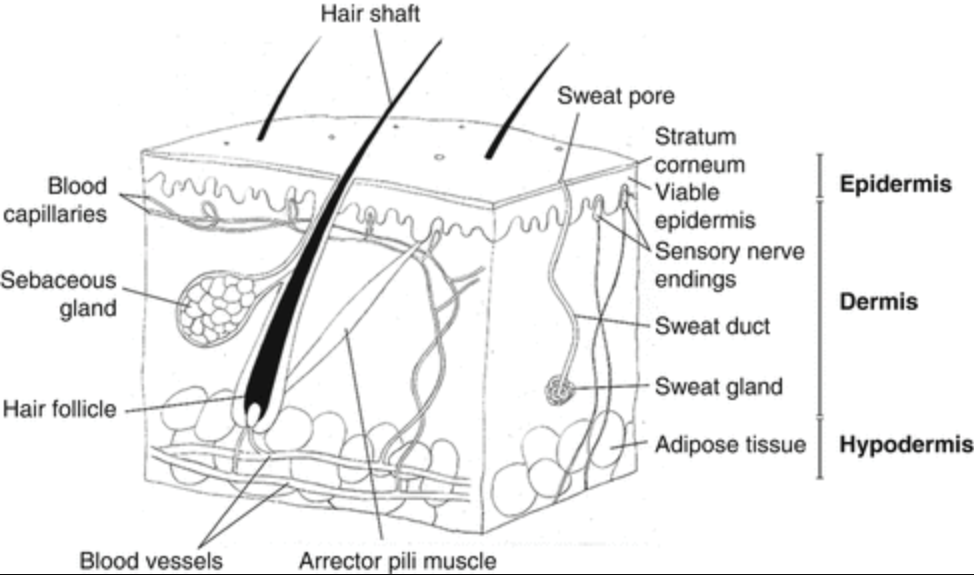
\includegraphics[width=0.95\linewidth]{img/przekroj_skory.png} 
    \caption{Skóra ludzka \cite{b_book_skin_photo}} 
    % \vspace{4ex}
  \end{subfigure}%% 
  \begin{subfigure}[t]{0.33\linewidth}
    \centering
    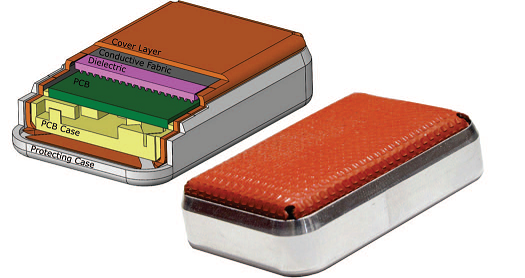
\includegraphics[width=0.95\linewidth]{img/przekroj_duck.png}
    \caption{Sztuczna skóra oparta na czujniku pojemnościowym \cite{b_konf_kaczka_przekroj}} 
    % \vspace{4ex}
  \end{subfigure}
  \begin{subfigure}[t]{0.33\linewidth}
    \centering
    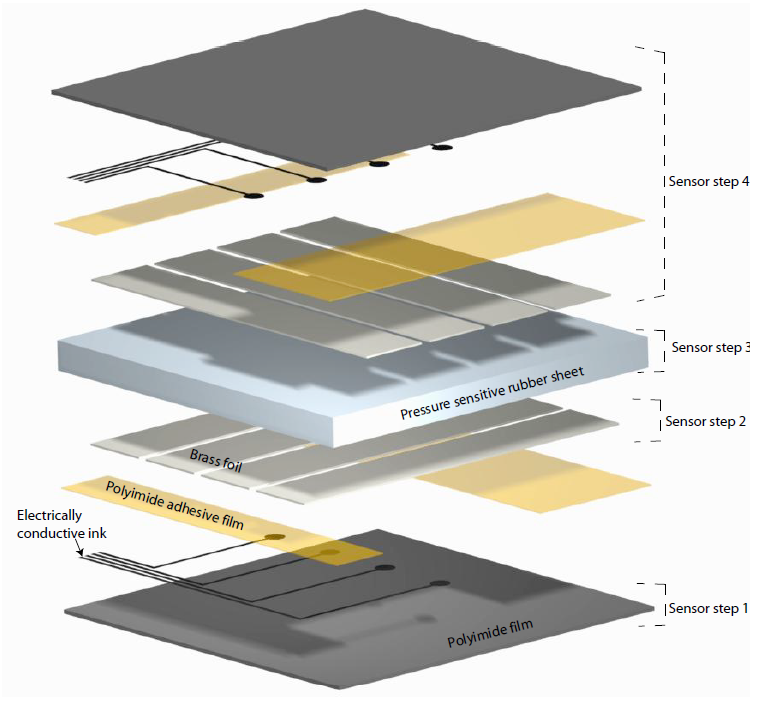
\includegraphics[width=0.95\linewidth]{img/przekroj_gietka.png}
    \caption{Sztuczna skóra oparta na warstwie o zmiennej rezystancji \cite{b_konf_gietka_przekroj}} 
    % \vspace{4ex}
  \end{subfigure}
  
  \centering
  \caption{Porównanie przekroju skóry ludzkiej i~przykładowych sztucznych skór}
  \label{f_porownanie_skory}
\end{figure}

Roboty asystujące to szczególny typ robotów przeznaczonych w~szczególności do wykonywania zleconych im zadań w~oparciu o aktualny stan siebie i~środowiska, bez ingerencji człowieka, ale we współpracy z~nim \cite{b_site_robot_definition}. Roboty asystujące z~racji na pełnione funkcje często są robotami mobilnymi posiadającymi sporą autonomiczność. Cechy te zapewniają robotowi możliwość samodzielnego poruszania się po otoczeniu oraz swobodne wykonywanie zleconych mu zadań. Swobodne poruszanie się po środowisku wymaga wykorzystywanie wielu czujników i~zabezpieczeń, aby robot nie wszedł w~kolizję ze środowiskiem. Przykładowymi kolizjami jakie mogą wystąpić są uderzenie w~ścianę bądź przedmiot lub też upadek z~krawędzi powierzchni (np. schodów). Środowisko pracy robotów asystujących jest dodatkowo utrudnione przez konieczność dzielenia jej z~istotami żywymi (ludźmi i~zwierzętami), które mogą się swobodnie poruszać lub modyfikować środowisko bez wiedzy robota.

Do pracy w~takim środowisku zachodzi potrzeba szerokiego wykorzystania wszelkiego rodzaju czujników odległości i~urządzeń mapujących otoczenie (np. LIDAR, laserowe czujniki odległości). Systemy te są szeroko wykorzystywane w~planowaniu trasy i~omijaniu przeszkód, nawet tych dynamicznie poruszających się. Systemy mapujące otoczenie są zazwyczaj umieszczane w~dolnych partiach robota, aby bardzo dobrze mapować podłoże, po którym porusza się robot. To podejście gwarantuje, że robot nie uderzy w~żaden stojący przedmiot, ani nie spadnie z~krawędzi. Problematyczna w~takim podejściu jest kwestia przedmiotów umieszczonych wyżej, które nie mają punktu podpierającego bezpośrednio pod sobą (np. blat stołu) lub są podwieszone na ścianie lub suficie. Roboty wyposażone w~czujniki na spodzie nie zawsze są w~stanie prawidłowo wykrywać tak umieszczone przeszkody.

Dodatkowo systemy wykrywające odległość nie są w~stanie bezpośrednio wykrywać wejścia robota w~kontakt z~otoczeniem. Są w~stanie wykryć tylko, że odległość robota do przeszkody jest mniejsza niż pozwala na to oprogramowanie, ale nie są w~stanie wykryć samej kolizji. W~takim wypadku (jeśli chcemy wykrywać kontakt) potrzebne nam jest rozwiązanie bazujące na sztucznej skórze. Sztuczna skóra jest zazwyczaj mocowana w~takim przypadku w~górnych partiach robota asystującego (dolna jest chroniona przez czujniki odległości), aby ochronić go przed uszkodzeniami i~pomagać mu omijać przeszkody, których nie jest w~stanie wykryć.

Robot asystujący będący już w~kontakcie z~przeszkodą może wykonać kilka akcji. Najprostszą jest zatrzymanie pracy - całkowite lub do momentu zakończenia nacisku. Jest to podejście, które poza faktem nieukończenia zadania może być niebezpieczne, ponieważ w~momencie zatrzymania robot cały czas wywiera nacisk na środowisko, potencjalnie na człowieka \cite{b_konf_collision_1}.
Innym podejściem jest wycofanie się w~miarę możliwości od elementu generującego nacisk do momentu jego zaniknięcia i~ponowne zaplanowanie nowej trasy wykonania zadania z~uwzględnieniem nowej niewykrytej wcześniej przeszkody. Podejście to zapewnia zarówno wykonanie zadania, jak i~akceptowalne oddziaływanie na środowisko.

Na rysunku \ref{f_przykladowe_roboty_uslugowe} widoczne są przykładowe roboty asystujące dostępne na rynku. Roboty przedstawione na tym rysunku przeznaczone są głównie do środowiska, gdzie muszą ściśle współpracować z~człowiekiem.

\begin{figure}[!h]
  \begin{subfigure}[t]{0.5\linewidth}
    \centering
    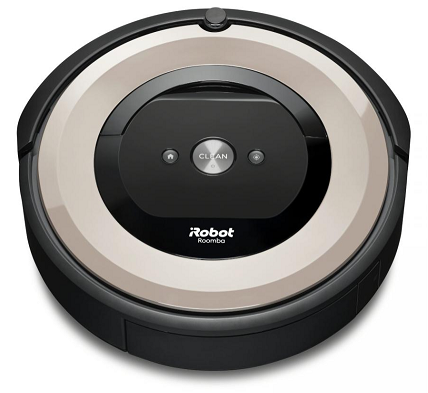
\includegraphics[width=0.7\linewidth]{img/robot_roomba.png} 
    \caption{Robot sprzątający Roomba \cite{b_site_roomba}} 
    % \vspace{4ex}
  \end{subfigure}%% 
  \begin{subfigure}[t]{0.5\linewidth}
    \centering
    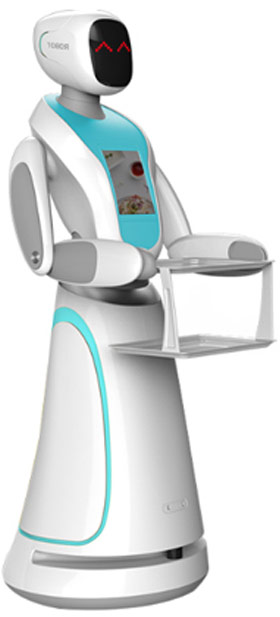
\includegraphics[width=0.4\linewidth]{img/robot_amy.jpg}
    \caption{Robot - kelner Amy \cite{b_site_Amy}} 
    % \vspace{4ex}
  \end{subfigure}
  
  \centering
  \caption{Przykładowe roboty asystujące dostępne na rynku}
  \label{f_przykladowe_roboty_uslugowe}
\end{figure}


\subsection{Motywacja}
Motywacją do wykonania prototypu sztucznej skóry była chęć rozwijania rozwiązań dotyczących sztucznej skóry, a w~szczególności wykonanie fizycznie działającej wersji i~zintegrowanie jej z~robotem. Dodatkowo chciałem poszerzyć zagadnienia związane z~problemami napotykanymi podczas budowy tego modułu robota i~testów, które trzeba wykonać na etapie planowania rozwiązania. 

Do wykonania pracy motywowała mnie również możliwość wykorzystania rozwiązania w~przyszłości w~robotach sprzedawanych powszechnie na rynku jako dodatkowa funkcja lub zabezpieczenie. Wykonany przeze mnie prototyp był testowany na robocie dostępnym na rynku, co pokazuje, że takie zastosowanie jest możliwe.

Motywacją była także chęć zintegrowania sztucznej skóry z~systemem ROS, co pozwala w~przyszłości zastosować ją na innych robotach opartych na tym systemie. 
% Zadanie to ułatwia możliwość zastosowanej zdalnej konfiguracji sterownika, którą może dokonać każdy przystosowując w~ten sposób rozwiązanie do swoich potrzeb. 
Użycie systemu ROS zwiększa także potencjalną bazę użytkowników i~ludzi, którzy mogliby dalej rozwijać wykonany przeze mnie model do innych zastosowań.

\subsection{Cel pracy}
% Prace prowadzone w~Zespole Programowania Robotów w~Zakładzie Sterowania Systemów, który funkcjonuje w~obrębie Instytutu Automatyki i~Informatyki Stosowanej na Wydziale Elektroniki i~Technik Informacyjnych na Politechnice Warszawskiej 
Prowadzone prace 
miały na celu zbudowanie sztucznej skóry wyczuwającej przykładany nacisk. Budowana skóra musiała być także jednocześnie prosta w~budowie, lekka, łatwo skalowalna, odporna mechanicznie i~możliwa do stosowania na nierównych powierzchniach.
Zbudowana sztuczna skóra miała za zadanie wspomagać robota asystującego w~poruszaniu się w~środowisku, w~szczególności chronić go przed obiektami i~uderzeniami. 
Zaproponowane rozwiązanie musiało też spełniać wymóg łatwej konfiguracji, która może być inna dla każdego zastosowania. Konfiguracja ta powinna odbywać się zdalnie, bez ingerencji w~program sterownika sztucznej skóry.

Celem pracy było również wykorzystanie zbudowanego czujnika w~praktyce poprzez umieszczenie go na robocie i~zintegrowanie go z~tym robotem. 
Integracja z~robotem miała pozwalać na zaprogramowanie robota, aby w~momencie wykrycia nacisku próbował uciec od jego źródła jeśli jest to możliwe.
% Integracja z~robotem miała pozwalać na zaprogramowanie na robocie dwóch różnych modeli zachowań:
% \begin{itemize}
%     \item wykrywanie nacisku i~próba odjechania od niego jeśli jest to możliwe
%     \item sterowanie kierunkiem ruchu robota dzięki naciskaniu na różne fragmenty skóry robota
% \end{itemize}

% Umieszczona na robocie sztuczna skóra miała za celu odbierać bodźce z~otoczenia i~przesyłać je w~przetworzonej formie do systemu sterującego robotem, aby ten podjął odpowiednie działania.

\subsection{Zakres pracy}
Praca obejmowała opracowanie prototypowego czujnika dotykowego zbudowanego jako sztuczna skóra wykrywająca siłę i~miejsce nacisku. Czujnik oparty był na folii rezystancyjnej Velostat znajdującej się pomiędzy przewodnikami elektrycznymi i~na jej właściwości do zmiany rezystancji pod wpływem przykładanego nacisku. Konstrukcja czujnika została zabezpieczona materiałem nośnym wykonanym z~gumy. Projekt ten był kontynuacją prac prowadzonych wcześniej przez Macieja Bogusza w~ramach Koła Naukowego Robotyki BIONIK \cite{b_report_otrzymane}.

Praca obejmowała przeprowadzenie badań nad wyborem optymalnego nośnika dla budowanego czujnika. Prowadzone badania obejmowały przetestowanie otrzymanego prototypu, kalibrację odczytów pomiarowych, budowę kolejnych prototypów potrzebnych do dalszych badań, jak również badanie właściwości różnych grubości użytych gum ochronnych. Badania obejmowały wykonanie charakterystyki folii Velostat w~wybranym zastosowaniu, pomiar pochłanialności energii poszczególnych grubości użytej gumy oraz rozkładanie energii wewnątrz czujnika.

Dodatkowo na potrzeby obsługi projektowanego czujnika konieczne było zaprojektowanie, wykonanie i~zaprogramowanie dedykowanego dla niego układu elektronicznego. Układ ten miał za zadanie przetwarzać dane odczytane ze sztucznej skóry i~w~przetworzonej formie przesyłać na stację roboczą - komputer z~systemem operacyjnym Linux Ubuntu do systemu sterującego robotem.

W zakres prac wchodziła także budowa sztucznej skóry zgodnie z~wynikami przeprowadzonych wcześniej badań oraz przetestowanie jej działania na fizycznie działającym robocie firmy PAL Robotics - Tiago \cite{b_site_tiago}, widocznym na rysunku \ref{f_tiago_zwykly}. Robot służący do testów działał pod kontrolą systemu ROS \cite{b_site_ROS}, więc jednym z~zadań było także dołączenie zbudowanego czujnika w~sposób kompatybilny z~wymaganiami stawianymi przez ten system.

\begin{figure}[!h]
    \centering 
    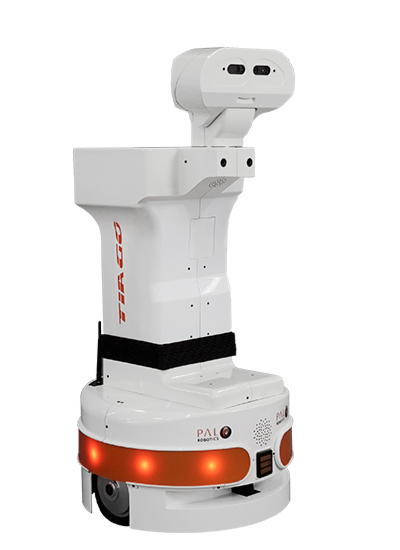
\includegraphics[width=0.5\linewidth]{img/tiago_zwykly.jpg}
    \caption{Robot Tiago \cite{b_site_tiago}}
    \label{f_tiago_zwykly}
\end{figure}

\subsection{Struktura pracy}
Niniejsza praca składa się łącznie z~ośmiu rozdziałów. W~pierwszym rozdziale zostały opisane założenia dotyczące końcowego celu jaki ta praca ma uzyskać. Opisany został też ogólny zakres prac wykonywanych podczas badań. Została także opisana motywacja jaka mną kierowała podejmując się wykonania niniejszej pracy.

Rozdział drugi opisuje przegląd istniejących na świecie rozwiązań dotyczących sztucznej skóry, jej budowy, badań nad nią i~zastosowanych rozwiązań. Zostały w~tym rozdziale opisane prace prowadzone przez innych naukowców na całym świecie i~możliwości zastosowanych przez nich podejść.

Rozdział trzeci zawiera kluczowe informacje dotyczące wykorzystanych narzędzi. Jest w~nim omówiony szczegółowo dobór zastosowanych komponentów, narzędzi i~systemów wykorzystywanych przez zbudowaną sztuczną skórę. W~tym rozdziale jest także opisana struktura systemu, do którego sztuczna skóra została dołączona i~robota, na którym była ona testowana.

Rozdział czwarty zawiera szczegółowy opis działania wybranego modelu sztucznej skóry i~podejście do zbudowania jej. W~tym rozdziale został szczegółowo przedstawiony otrzymany prototyp i~prace jakie nad nim zostały wykonane. Opisana została także budowa pozostałych warstw projektowanej przeze mnie wersji, ze szczególnym skupieniem się na sterowniku sztucznej skóry - jego elektronice i~oprogramowaniu.

% Rozdział piąty opisuje wykonane prace nad sterownikiem obsługującym projektowaną sztuczną skórę. Został opisany proces projektowania dedykowanego układu elektronicznego i~sposób obsługiwania przez niego sztucznej skóry wraz z~omówieniem wykonanego oprogramowania mikrokontrolera. Znajduje się tutaj także specyfika komunikacji układu z~komputerem nadrzędnym.

Rozdział piąty został poświęcony procesowi badań nad doborem optymalnych materiałów do budowy sztucznej skóry. Badania te prowadzone były na statycznej wersji dodatkowych mniejszych prototypów. Szczegółowo została opisana tutaj kwestia doboru odpowiedniego materiału nośnego będącego jednocześnie warstwą ochronną sztucznej skóry.

Rozdział szósty opisuje integrację sztucznej skóry z~istniejącym systemem robota. W~rozdziale tym można znaleźć szczegóły konfiguracji robota Tiago wykorzystywanego w~testach oraz proces podłączania do niego sztucznej skóry. Została także krótko opisana budowa mechaniczna zbudowanej sztucznej skóry.

Przedostatni rozdział - siódmy prezentuje wykonane testy zbudowanego czujnika, zarówno w~symulacji jak i~w~realnych warunkach. Zawarta jest w~nim weryfikacja poprawności działania w~obu tych warunkach. Przedstawiony został także drugi prototyp sztucznej skóry wraz z~powodami konieczności tworzenia kolejnej wersji czujnika.

Rozdział ósmy stanowi podsumowanie pracy. Zawarte jest w~nim podsumowanie wykonanych celów i~prac. W~rozdziale zostały także opisane wnioski jakie można wyciągnąć z~wykonanych prac.
         % Wygodnie jest trzymać każdy rozdział w osobnym pliku.
% \input{tex/2-de-finibus}    % Umożliwia to również łatwą migrację do nowej wersji szablonu:
% \input{tex/3-code-listings} % wystarczy podmienić swoje pliki main.tex i eiti-thesis.cls
                            % na nowe wersje, a cały tekst pracy pozostaje nienaruszony.
\newpage
\section{Przegląd istniejących rozwiązań w zakresie sztucznej skóry}
\label{s_przeglad}

\subsection{Dostępne metody wykrywania dotyku}

Podstawą w budowie sztucznej skóry jest możliwość wykrywania bodźców zewnętrznych. O ile pomiary temperatury, pod względem dalszej użyteczności, nie muszą posiadać dużej rozdzielczości pomiaru o~tyle rzecz ma się całkiem inaczej jeśli chodzi o wykrywanie nacisku. To właśnie miejsce i siła nacisku jest kluczową informacją jakiej oczekujemy od sztucznej skóry. W zależności od przeznaczenia i możliwości, do budowy wykorzystywane są różne materiały oraz metody produkcji. Do wykrywania nacisku wykorzystywane są różne zjawiska mechaniczne, elektryczne a nawet chemiczne. Istnieją także różnice w~sposobie przesyłania sygnałów w samym czujniku, jak i do układu sterowania robotem. Wszystkie wybrane metody powinny ze sobą współpracować i się uzupełniać wewnątrz wybranego rozwiązania.

Zazwyczaj wyborem, do którego dostosowywane są pozostałe jest sposób wykrywania i pomiaru siły nacisku. To on definiuje możliwości i typy użytej warstwy ochronnej. On~również definiuje jakie układy elektroniczne zostaną użyte do obsługi sztucznej skóry oraz sposób połączenia czujników nacisku z elektroniką sterującą. Możliwych metod pomiaru nacisku jest wiele, ale najbardziej powszechnymi są:
\begin{itemize}
    \item pojemościowe - pomiar zmieniającej się pojemności,
    \item rezystancyjne - pomiar zmieniającej się rezystancji,
    \item piezoelektryczne - pomiar skokowych zmian napięcia,
    \item indukcyjne - pomiar zmian natężenia pola magnetycznego,
    \item optyczne - pomiar natężenia światła lub jego barw składowych.
\end{itemize}

Do tych rzadziej spotykanych należą niewątpliwie układy MEMS o małym rozmiarze oraz dużo większym stopniu skomplikowania. Spotykane też są rozwiązania hybrydowe, które oprócz standardowych metod pomiaru wspomagają się układami MEMS oraz żywymi komórkami i tkankami \cite{b_article_reviev_tactile_skin}. Nie są to jednak rozwiązania, które aktualnie są stosowane w robotyce ze względu na swój koszt oraz skomplikowanie w wytwarzaniu.

Czujniki pojemnościowe są najprawdopodobniej najczęściej wykorzystywane do pomiaru nacisku. Ich główną zasadą działania jest pomiar pojemności pomiędzy dwoma warstwami przewodnika oddzielonymi dielektrykiem. W praktyce zmiana pojemności wywoływana jest przez zmianę grubości dielektryka (uginanie go) \cite{b_konf_kaczka_przekroj}. Zmiana grubości tej okładki wynika bezpośrednio z przyłożonego do sztucznej skóry nacisku. Czujniki pojemnościowe są tak często wybierane ze względu na swoją wysoką czułość, łatwość budowy, dużą rozdzielczość oraz odporność mechaniczną. Czujniki te wymagają jednak do pracy specjalistycznych układów elektronicznych znanych jako CDC (capacitance to digital converter), które niewątpliwie utrudniają zastosowanie w praktyce \cite{b_article_reviev_2_tactile_skin, b_konf_wloch_1_opis_budowy}.

Innym również często spotykanym sposobem wykrywania nacisku jest wykorzystanie zmieniającej się rezystancji materiału pod wpływem nacisku. Rozróżniane są tutaj czujniki piezorezystancyjne oraz tensometryczne, przy czym te drugie, ze względu na zależność od fizycznego odkształcenia czujnika, są rzadko wykorzystywane. Wykorzystywane i~budowane są natomiast czujniki w oparciu o wykorzystanie materiałów piezorestywnych i pomiarze zmian ich rezystancji w zależności od przyłożonej siły. Pozwala to na skonstruowanie czujnika o praktycznie dowolnej wielkości i kształcie. Układ pomiarowy, w~przeciwieństwie do czujników pojemnościowych, jest bardzo prosty, a same pomiary bardzo czułe na zmiany. Niestety układy mierzące rezystancję pobierają z reguły dużo prądu, co czyni je nie najlepszym wyborem w zastosowaniach o niskim zużyciu energii. Układy te również cechują się stosunkowo długim czasem pomiaru i dużą rozbieżnością pomiarów \cite{b_article_reviev_tactile_skin, b_article_reviev_2_tactile_skin, b_konf_tactile_resist_review}.

W robotyce do pomiaru nacisku spotykane jest także wykorzystywanie czujników piezoelektrycznych. Zbudowane są one ze specjalnych polimerów, które pod wpływem nacisku generują ładunek elektryczny lub napięcie, które jest później mierzone. W zależności od zmierzonej wartości można wnioskować jak mocna wystąpiła zmiana nacisku. Czujniki piezoelektryczne nadają się jednak tylko do pomiarów dynamicznych - nie są w~stanie wykryć statycznie przykładanej siły. Ta cecha może być zaletą, ponieważ eliminuje konieczność kalibracji do warunków podczas uruchamiania. Zazwyczaj jednak jest to wada, ponieważ nie jesteśmy w stanie wykryć nawet dużych sił, jeśli nie zmieniają one swojej wartości. Są to natomiast czujniki bardzo odporne na czynniki środowiskowe i~zapewniają bardzo szybki odczyt \cite{b_article_tactile_piezo, b_article_reviev_tactile_skin, b_article_reviev_2_tactile_skin}.

Czujniki indukcyjne również są wykorzystywane do wykrywania nacisku. Ich działanie polega na tworzeniu pola magnetycznego z wykorzystaniem cewek i monitorowaniu jego zmian. Przyłożenie nacisku powoduje ugięcie powierzchni przewodzącej prąd, jednocześnie zmieniając właściwości pola magnetycznego wewnątrz czujnika. Te właśnie zmiany są wykrywane i ich charakterystyka wykorzystywana jest w dalszej obróbce sygnału. Pomiar ten zapewnia szybkie i stosunkowo dokładne pomiary nacisku. Największą wadą czujników indukcyjnych, wykluczającą ją z większości zastosowań, jest konieczność stosowania w środowisku wolnym od materiałów wpływających na pole magnetyczne. Poza tym układy te pobierają sporo energii, a do ich obsługi potrzebna jest specjalistyczna elektronika \cite{b_article_tactile_inductive, b_article_reviev_tactile_skin}.

Ostatnim z najczęściej spotykanych sposobów pomiaru nacisku są czujniki optyczne i te bazujące na pomiarze zmiany parametrów wiązki światła. Ogólna zasada działania jest bardzo prosta i polega na wysyłaniu wiązki świetlnej przez przezroczysty ośrodek, a~następnie odbieranie wiązki z drugiej strony ośrodka. Ośrodek ten jednak jest podatny na nacisk i pod jego wpływem zmienia swoje właściwości, deformując przechodzącą przez niego wiązkę światła. Deformacje te mogą polegać na zmianie ilości przepuszczanego światła lub jego widmie. Czujniki te są w~stanie wykrywać bardzo małe siły oraz są w~pełni odporne na zakłócenia pochodzące ze środowiska zewnętrznego.
Budowa czujnika musi być jednak wykonana bardzo precyzyjnie, aby nie pogarszać właściwości czujnika i~zachować niewielkie rozmiary (czujniki optyczne są trudne i drogie do zminiaturyzowania) \cite{b_konf_tactile_opto, b_article_reviev_tactile_skin, b_article_reviev_2_tactile_skin}.


\subsection{Modułowa sztuczna skóra przeznaczona dla robotów humanoidalnych}

%Co, gdzie, czy i jak działa, wady zalety, zastosowanie

Jednym z lepiej wykonanych i szeroko testowanych przykładów sztucznej skóry jest ten rozwijany we Włoszech na Uniwersytecie Genueńskim. Jest to projekt rozwijamy od wielu lat, który w założeniach miał być stosowany w robotach humanoidalnych jako dodatkowe zabezpieczenie podczas pracy. Jednym z głównych efektorów robota humanoidalnego są manipulatory, które z uwagi na swoją charakterystykę pracy posiadają ruchome stawy, które to znacząco utrudniają wykorzystanie sztucznej skóry w okolicach zgięć robota. Dodatkowo, manipulatory posiadają zazwyczaj dużą potencjalną powierzchnię kolizji, która dodatkowo mocno się zmienia podczas pracy robota \cite{b_konf_wloch_1_opis_budowy}. 

Aby sprostać tak wysokim wymaganiom, do budowy sztucznej skóry zostały wybrane czujniki pojemnościowe wraz z przemysłowymi przetwornikami CDC (capacitance to digital converter, przetwornik pojemnościowo-cyfrowy). Dużą uwagę położono także na modułowości wybranego rozwiązania i możliwości bardzo łatwej i szybkiej rozbudowy całego systemu poprzez wykorzystanie większej liczby modułów. Na zbudowanym prototypie zostało także przeprowadzone szereg badań pod kątem zależności odczytów od~czynników zewnętrznych. Badania te pokazały dobrą stabilność pomiarów i pozwoliły na wykonanie dokładnej charakterystyki sztucznej skóry 
\cite{b_article_wloch_4_wytrzymalosc, b_konf_wloch_1_opis_budowy}. Przekrój budowy pojedynczego modułu czujnika oraz sposób łączenia modułów ze sobą został przedstawiony na rysunku \ref{f_triangle_1-2-3}. Na zdjęciach można zauważyć jak blisko siebie położone są kolejne pola pomiarowe. Warstwa dielektryka pełni w tym rozwiązaniu nie tylko funkcję przenoszenia informacji, ale również chroni robota przed potencjalnymi uszkodzeniami. Takie rozłożenie pozwoliło zrealizować na kolejnych etapach prac miarodajne i rzetelne badania \cite{b_konf_wloch_1_opis_budowy}.

\begin{figure}[!h]
  \begin{subfigure}[t]{0.55\linewidth}
    \centering
    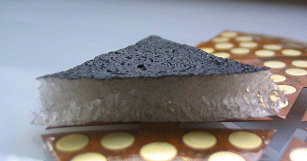
\includegraphics[width=0.95\linewidth]{img/triangle2.png}
    \caption{Budowa pojedynczego modułu sztucznej skóry} 
    % \vspace{4ex}
  \end{subfigure}
  \begin{subfigure}[t]{0.4\linewidth}
    \centering
    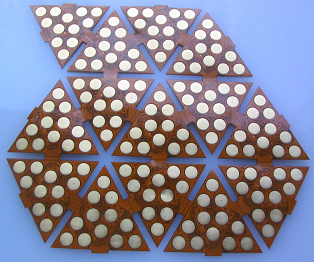
\includegraphics[width=0.83\linewidth]{img/triangle3.png}
    \caption{Sposób łączenia modułów sztucznej skóry} 
    % \vspace{4ex}
  \end{subfigure}
  
  \centering
  \caption{Prototyp modularnej sztucznej skóry projektowanej do robota humanoidalnego \cite{b_konf_wloch_1_opis_budowy}}
  \label{f_triangle_1-2-3}
\end{figure}

Zaprojektowane rozwiązanie zostało w praktyce przetestowane na robocie Baxter, na jednym z jego ramion, gdzie zostało zamocowane aż 768 czujników pojemnościowych \cite{b_site_baxter}. Na umieszczonym tak prototypie zostały wykonane testy idące dużo dalej niż samo wykrywanie nacisku. Na podstawie danych otrzymywanych z modułów rozpoznawane były kształty, jakie są przykładane do robota, czym w przypadku testów było różne ułożenie dłoni na robocie. Surowe dane przed dalszą obróbka są przekształcane do postaci obrazu trójwymiarowego uwzględniającego położenie każdego z czujników w przestrzeni.
Na tym etapie uwzględniane są także położenia poszczególnych stawów robota względem siebie, co pozwala na prawidłową identyfikację nacisku w stawach robota.
Do celów rozpoznawania wzorców na sztucznej skórze została wykorzystana konwolucyjna sieć neuronowa osiągająca skuteczność do $97\%$
\cite{b_konf_wloch_2_reka, b_konf_wloch_3_reka}. Na rysunku \ref{f_triangle_test} jest widoczna sztuczna skóra zamocowana na robocie oraz jej testy na robocie.

\begin{figure}[!h]
  \begin{subfigure}[t]{0.36\linewidth}
    \centering
    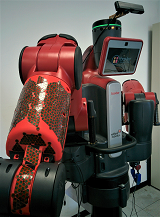
\includegraphics[width=0.95\linewidth]{img/triangle4.png}
    \caption{Robot Baxter z zamocowaną podstawą sztucznej skóry} 
    % \vspace{4ex}
  \end{subfigure}
  \begin{subfigure}[t]{0.62\linewidth}
    \centering
    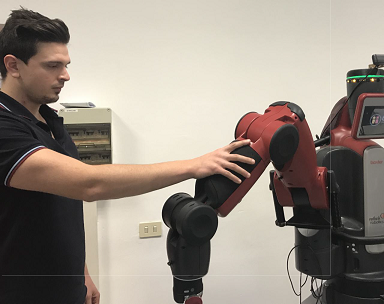
\includegraphics[width=0.95\linewidth]{img/triangle5.png}
    \caption{Sztuczna skóra na robocie podczas testów} 
    % \vspace{4ex}
  \end{subfigure}
  
  \centering
  \caption{Prototyp modularnej sztucznej skóry testowanej na robocie \cite{b_konf_wloch_2_reka}}
  \label{f_triangle_test}
\end{figure}

Zaprojektowane we Włoszech rozwiązanie może w przyszłości być stosowane powszechnie w robotach humanoidalnych. Jest to nie tylko bardzo dobre zabezpieczenie przed wejściem robota w kolizję z otoczeniem lub człowiekiem przy nim pracującym, ale również pozwala na zdalne sterowanie ruchami robota poprzez wykrywanie ułożeń dłoni operatora na skórze robota. Stopień zaawansowania prac nad rozwiązaniem pozwala na założenie, że w ciągu kilku najbliższych lat podobne rozwiązanie pojawi się na rynku. 


% ZA: An Embedded Artificial Skin for Humanoid Robots  Giorgio Cannata, Marco Maggiali, Giorgio Metta and Giulio Sandini

% ZB: On the Recognition of Human Hand Touch from Robotic Skin Pressure Measurements Using Convolutional Neural Networks  Alessandro Albini, Simone Denei and Giorgio Cannata

% ZC: Tactile Images Generation from Contacts Involving Adjacent Robot Links  Alessandro Albini1 and Giorgio Cannata

% ZD: A Flexible and Robust Large Scale Capacitive Tactile System for Robots   Perla Maiolino, Marco Maggiali, Giorgio Cannata, Giorgio Metta, and Lorenzo Natale


\subsection{Elastyczna sztuczna skóra do środowisk współpracy z człowiekiem}

Roboty pracujące pośród ludzi, jak pokazał wcześniej opisany przykład, muszą zapewnić człowiekowi bezpieczeństwo podczas pracy robota. Kluczowe jest więc pokrycie sztuczną skórą wykrywającą nacisk jak największej powierzchni obudowy robota. Pokrycie dużej powierzchni wiąże się jednak z koniecznością użycia dużej liczby czujników i mocy obliczeniowej do przetworzenia w czasie rzeczywistym otrzymywanych danych. Zminimalizowanie tych dwóch czynników jest więc pożądane w przemyśle, aby możliwie mocno zmniejszyć koszty bez straty bezpieczeństwa pracy. Rozwiązanie tego problemu zostało zaproponowane przez naukowców z kanadyjskiego Uniwersytetu Lavala w Quebec. Ich głównymi założeniami przy projektowaniu sztucznej skóry były niski koszt wytworzenia i~możliwość szybkiej reakcji na otrzymane bodźce
\cite{b_konf_gietka_przekroj}.
% W przypadku robotów, których przeznaczeniem będzie wykorzystanie do pracy z ludźmi, bardzo istotną kwestią jest bezpieczeństwo podczas interakcji robot-człowiek. Kluczową funkcją, która mogłaby zwiększyć poziom ochrony człowieka przed ewentualnymi wypadkami, jest zapewnienie wykrywania kontaktu na całym ciele robota (lub na jego najbardziej narażonych na kolizję z człowiekiem elementach). Nad tym problemem pochylili się naukowcy pracujący w Departamencie Inżynierii Mechanicznej Uniwersytetu Lavala w Kanadzie. Dodatkową motywacją stojącą za zaproponowanym przez nich projektem było wyprodukowanie stosunkowo niedrogiej powłoki, która byłaby w stanie zapewnić przestrzenną lokalizację kolizji robota z otoczeniem i szybką reakcję na nią. Rozwiązanie, które skonstruowali, to w praktyce cienki elastyczny arkusz czujnika wykonany z folii poliimidowych z tuszem przewodzącym prąd oraz gumową warstwą wrażliwą na nacisk. Poza niską ceną, dużą zaletą zaproponowanego rozwiązania jest brak konieczności prowadzenia przewodów wewnątrz czujnika. Problem ten ominięty został przez zastosowanie przewodzącego tuszu. Zaproponowany obwód mocno minimalizuje liczbę przewodów wyjściowych \cite{b_konf_gietka_przekroj} \cite{b_book_gietka_source_1}.% CITE AS: a, b

Zastosowany czujnik swoje działanie opiera na pomiarach rezystancji specjalnej folii znajdującej się wewnątrz. W zaproponowanym rozwiązaniu, dwie przewodzące płaszczyzny są oddzielone od siebie materiałem wrażliwym na nacisk. Bez obciążenia zewnętrznego posiada on bardzo dużą rezystancję, która wraz z przykładaniem coraz większego nacisku stopniowo się zmniejsza. Same przewodzące płaszczyzny są w praktyce równolegle ułożonymi pasmami przewodzącymi. Pasma na przeciwnych płaszczyznach są~ułożone względem siebie prostopadle. Cały schemat budowy jest dobrze zobrazowany na rysunku \ref{f_przeglad_gietka_przekroj}, który prezentuje schematyczne ułożenie poszczególnych warstw wewnątrz czujnika. Na zewnątrz widoczne są~także warstwy ochronne czujnika znajdującego się wewnątrz. Dużą zaletą zaproponowanego rozwiązania jest wykorzystanie specjalnych tuszów przewodzących prąd, co pozwoliło na znaczne ograniczenie konieczności stosowania przewodów. Zbudowany czujnik został dodatkowo zalany w żywicy, aby uodpornić go na warunki zewnętrzne i~zapewnić większą trwałość \cite{b_konf_gietka_przekroj}.

\begin{figure}[!h]
    \centering 
    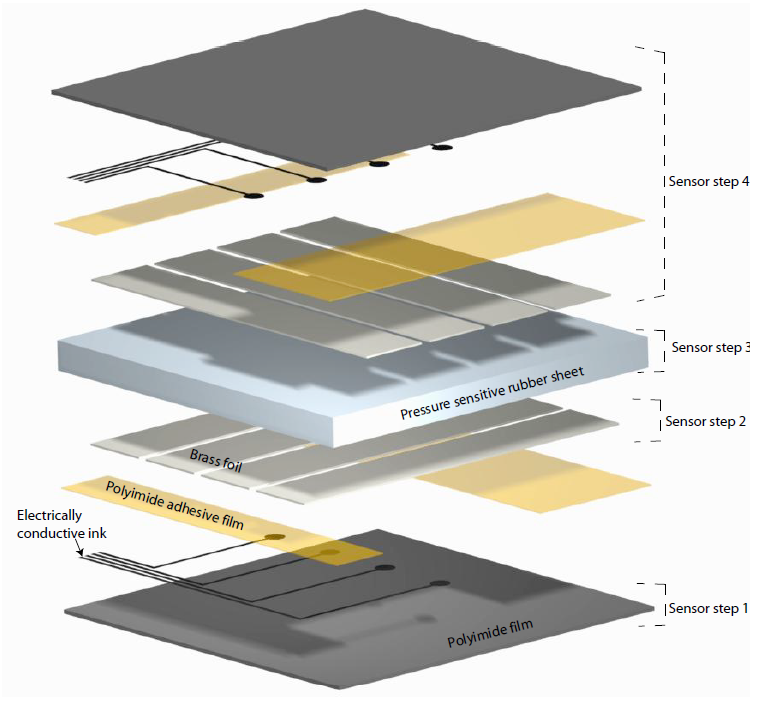
\includegraphics[width=0.4\linewidth]{img/przekroj_gietka.png}
    \caption{Schemat ułożenia poszczególnych warstw sztucznej skóry \cite{b_konf_gietka_przekroj}}
    \label{f_przeglad_gietka_przekroj}
\end{figure}


% Następnie, czujnik został osadzony między dwoma warstwami poliuretanu o różnej twardości Shore'a (30A oraz 20A) przy użyciu technologii osadzania kształtu (ang. \textit{shape deposition manufacturing}, SDM). Badacze wykorzystali takie rozwiązanie, aby zapewnić jak najlepsze tłumienie kolizji oraz wytrzymałość mechaniczną. Wytworzona w ten sposób warstwa skóry może w małym stopniu wyginać się bez tworzenia się uszkodzeń. Zauważono jednak, że powyżej pewnego wygięcia wewnętrzne naprężenia materiału mogą aktywować czujnik, co powoduje otrzymanie błędnych odczytów informujących o kontakcie robota z przeszkodą. Rozwiązaniem tego problemu może być wytwarzanie skóry w zakrzywionej formie. % CITE AS: c 
% tu można dodać rys ze schematem tego zatapiania, ale no nie wiem. Ja bym dodała, ale z pierwszym rysunkiem już tego jest około 1 strony opisu 

Na wykonanym prototypie przeprowadzono szereg testów mających na celu określenie zalet i wad wykonanego rozwiązania, jak również wyznaczenie jego charakterystyki pracy. Ogólne testy przebiegły pomyślnie i nie wykazały większych wad poza faktem, że prototyp przy mocniejszym zginaniu wysyła sygnały mogące świadczyć o kontakcie z przeszkodą, której nie ma. Jest to spowodowane tym, że czujnik nie rozpoznaje pochodzie naprężeń obecnych na swojej powierzchni. Rozwiązaniem tego problemu może być wytwarzanie skóry, która naturalnie posiada swoją krzywiznę \cite{b_konf_gietka_przekroj}.

Opisywane rozwiązanie jest dobrym krokiem w kierunku produkcji taniej powłoki wykrywającej kontakt na robotach przemysłowych, lecz przed doprowadzeniem go do użycia komercyjnego potrzebne jest wykonanie dalszych badań. Ten prototyp był w dużej mierze inspiracją i jedną z podstaw do zbudowania prototypu czujnika opisywanego w~kolejnych rozdziałach pracy.

% Po wykonaniu prototypów przeprowadzono serię eksperymentów, aby zweryfikować wartość progową nacisku na wytworzoną skórę. Siła aktywacji czujnika, którą należało przyłożyć, wahała się od $0,5 N$ do $5 N$ dla powierzchni styku $32 mm^2$, co skutkowało progowym ciśnieniem w granicach $15,8 kPa$ do $158 kPa$. Różne odczyty uzyskiwano w zależności od miejsca przyłożenia siły. Wartość progowa nacisku jest funkcją grubości materiału, użytego rodzaju materiału warstwy zewnętrznej, gęstości z basowej warstwie zewnętrznej (twardości warstwy poliuretanu) oraz właściwości fizycznych warstwy materiału wrażliwego na nacisk umieszczonego między płytkami przewodzącymi. Przez zmianę właściwości tych parametrów w projekcie można więc dostosowywać wartości progowej do pożądanych wielkości. % CITE AS: a

% a: V. Duchaine, N. Lauzier, M. Baril, M.-A. Lacasse and C. Gosselin. "A flexible robot skin for safe physical human robot interaction". Robotics and Automation 2009. ICRA '09. IEEE International Conference on, pp. 3676-3681, May 2009. (mat pokonferencyjne)

% b: M. R. Cutkosky, R. D. Howe, and W. R. Provancher, “Force and tactile sensors,” Springer Handbook of Robotics, pp. 455–476, 2008.

% c: M. Hatanaka and M. Cutkosky, “Process planning for embedding flexible materials in multi-material prototypes,” DETC ASME, Chicago, Illinois, USA, September, 2003. (mat pokonferencyjne)


\subsection{Sztuczna skóra wysokiej rozdzielczości wykorzystywana w chwytakach}

% h jednak nie bedzie cytowane

Roboty wykorzystywane są czasami do przenoszenia lub przekładania różnych przedmiotów. Aby wykonywać to sprawnie potrzebują one odpowiednich chwytaków do chwytania przedmiotów. Dodatkowym plusem są chwytaki wyposażone w sztuczną skórę, która pozwala na rozpoznawanie przedmiotów lub przenoszenie ich z odpowiednią ostrożnością. Sztuczna skóra użyta na chwytakach musi się więc charakteryzować wysoką czułością i elastycznością, aby idealnie dopasować się do podnoszonego przedmiotu.
% Czujniki stosowane w robotach z modułem chwytającym muszą charakteryzować się wysoką wydajnością. W przypadku tego typu rozwiązaniach można napotkać wiele problemów związanych z różną strukturą czy elastycznością łapanych przez roboty obiektów. Wyzwaniem mogą też być takie zdarzenia jak poślizg czy utrata kontaktu. 

Sztuczna skóra dostosowana do tego użycia jest rozwijana na Wyższej Szkole Technologicznej w Montrealu w Kanadzie. Sztuczna skóra została zaprojektowana tak, aby~odpowiednio eliminować kolejne potencjalne problemy w użytkowaniu czujnika. Ogólna budowa czujnika jest bardzo prosta i opiera się na pomiarze pojemności, ale ogromną wagę przyłożono do materiałów i~struktur obudowujących czujnik. Jako dielektryk został wykorzystany standardowy elastyczny materiał (oparty na silikonie), ale uformowany w regularne wypustki, które poprawiają charakterystykę pracy czujnika, zwiększają elastyczność pracy oraz pomagają w utrzymaniu niskiej masy powłoki. 
Przekrój budowy czujnika sztucznej skóry, jak również zasada działania elastycznych wypustek dielektryka przedstawiona jest na rysunku \ref{f_przekroj_duck} \cite{b_konf_kaczka_przekroj}.

% Stworzona przez nich sztuczna skóra swój sukces opiera na zastosowaniu rozwiązania, w którym czujniki statyczne i dynamiczne są zintegrowane w tej samej warstwie czujnika pojemnościowego z umieszczoną bezpośrednio nad nim warstwą mikrostrukturalnego dielektryka. Czujniki statyczne odpowiadają za odczyt informacji o lokalizacji nacisku (zarówno normalnej siły, jak i naprężeń ścinających), podczas gdy czujniki dynamiczne odnoszą się do wszystkich zdarzeń kontaktowych, takicj jak poślizg czy rozpoznawanie obiektów. % CITE AS: g
% ??? 'static and dynamic sensing are integrated in the same layer of capacitive sensor with direct written microstructured dielectric'     czy ja to dobrze tlumacze? 

% Materiał dielektryczny w niniejszym projekcie stanowi warstwa silikonu, w którym umieszczone zostały nanocząsteczki materiału przewodzącego, którym jest tytanian baru ($BaTiO_3$). Wykorzystanie tego połączenia zostało doświadczalnie uzasadnione. W porównaniu z innymi dielektrykami używanymi w podobnych rozwiązaniach tytanian baru wykazał najlepsze właściwości. Nie powodował nadmiernej utraty właściwości fizycznych silikonu, jest ogólnie dostępny i kilkukrotnie tańszy od innych materiałów o podobnych właściwościach.  % CITE AS: i
% Silikon z dodatkiem tytanianu baru wprowadzany jest do formy akrylowej nadającej mu wyjątkowy kształt, który ma kluczowe znaczenie w powodzeniu tego konceptu. Powstała warstwa ma kształt arkusza z równomiernie rozmieszczonymi mikrowypustkami o kształcie ściętego stożka. Każda z wypustek ma podstawę o średnicy $0,6 mm$, płasko ściętą końcówkę o średnicy $0,3 mm$ oraz wysokość $0,5 mm$. Odległość między środkami położonych sąsiadująco wypustek to $1,2 mm$. Strona pokryta wypustkami zwrócona jest w stronę płytki PCB przylegając do niej. Po przyłożeniu ciśnienia wypustki ulegają szybkiej reformacji i rozszerzaniu się dotykając płytki coraz większą powierzchnią. Rysunek \ref{f_przeglad_mikrowypustki} przedstawia schematycznie zachowanie mikrowypustek pod wpływem działania siły na warstwę dielektryka. 

\begin{figure}[!h]
  \begin{subfigure}[t]{0.49\linewidth}
    \centering 
    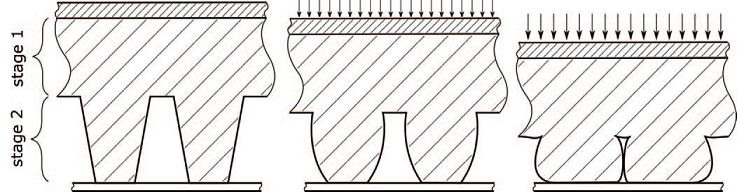
\includegraphics[width=0.95\linewidth]{img/duck_silikon.png}
    \caption{Budowa i działanie wypustek dielektryka}
    % \vspace{4ex}
  \end{subfigure}
  \begin{subfigure}[t]{0.49\linewidth}
    \centering 
    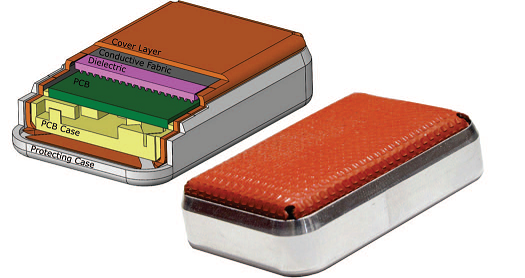
\includegraphics[width=0.95\linewidth]{img/przekroj_duck.png}
    \caption{Przekrój budowy czujnika sztucznej skóry}
    % \vspace{4ex}
  \end{subfigure}
  
  \centering
  \caption{Przekrój budowy dokładnego czujnika sztucznej skóry \cite{b_konf_kaczka_przekroj}}
  \label{f_przekroj_duck}
\end{figure}

Spory uwagę przyłożono także do odpowiedniej budowy części czujnika pojemnościowego znajdującego się na PCB. Zostało przetestowane kilka różnych sposobów prowadzenia ścieżek, które były sprawdzane pod kątem jak najlepszych otrzymywanych odczytów, zarówno statycznych, jak i~dynamicznych. Przeprowadzono również standardowe testy na stabilność pracy w różnych temperaturach, kalibrację czujnika oraz szybkość reakcji. Przeprowadzone doświadczenia potwierdziły zasadność prowadzonych badań oraz doprowadziły do zbudowania pełnego prototypu sztucznej skóry. Prototyp ten został umieszczony do dalszych eksperymentów na chwytaku firmy Robotiq \cite{b_konf_kaczka_przekroj}.

Obserwując postęp prac jest to bardzo obiecujące rozwiązanie, które z powodzeniem będzie wykorzystywane w różnych chwytakach robotycznych ze względu na swoją precyzję oraz elastyczność. Jego głównymi wadami są trudna skalowalność i stosunkowo wysoki koszt produkcji, które to bardzo utrudniają wyposażenie robota w opisywaną sztuczną skórę na całej jego powierzchni.

% wady zalety, zastosowanie

% Zmiany w budowie warstwy przewodzącej nie były jedynymi innowacjami wprowadzonymi przez badaczy do tego projektu. Zaproponowali oni również nowatorski sposób ułożenia sensorów na płytce PCB. Większość dotykowych czujników pojemnościowych posiada kwadratowe taksele. % taxel/pixel - nie wiem jak to przetlumaczyc 
% W przypadku czujników multimodalnych, gdzie należy zastosować dwa typy //takseli??// użycie tego kształtu prowadziłoby do niejednolitej wrażliwości na dotyk w różnych miejscach czujnika. Aby zapobiec temu problemowi zaprojektowano czujnik z //takselami// w kształcie grzebienia, co pozwala na przeplatanie się dwóch rodzajów czujników. % CITE AS: g

% Konstrukcja ta posiada ulepszoną konstrukcję elektryczną i mechaniczną w stosunku do rozwiązań zaproponowanych uprzednio przez innych naukowców. Dzięki temu etap produkcji zostaje uproszczony. Przedstawione rozwiązanie może być z powodzeniem wykorzystane w precyzyjnych robotach wyposażonych w chwytaki. 

\subsection{Sztuczna skóra wykrywająca odkształcenia w trzech osiach}

%Co, gdzie, czy i jak działa, wady zalety, zastosowanie

Ciekawym rozwiązaniem, które może mieć swoje zastosowanie nie tylko w robotyce, ale również w niektórych dziedzinach medycyny, jest projekt w pełni elastycznej sztucznej skóry. Ten wysoce zaawansowany prototyp jest rozwijany na Uniwersytecie Harwardzkim we współpracy z Instytutem Wyssa zajmującego się inżynierią biologiczną. Czujnik ten w~praktyce jest zaawansowanym czujnikiem rezystancyjnym, którego pomiary kolejnych rezystancji są ze sobą mocno skorelowane. 

Zaproponowana sztuczna skóra składa się z trzech warstw mikrokanałów utworzonych w silikonowej formie, które wypełnione są płynną (w temperaturze pokojowej) cieczą przewodzącą prąd. Jako materiał przewodzący wykorzystany został eutektyczny stop galu i indu (EGaIn) \cite{b_article_EGaIn}. Pole czujnika jest małych rozmiarów ($25x25x3,5mm$) oraz jest mocno rozciągliwe. Wymienione cechy pozwalają mu na wykrywanie przykładanego nacisku w~wielu osiach \cite{b_article_tactile_precise}.

Budowa czujnika jest prosta w założeniach, a jej skomplikowanie wynika głównie z~niewielkich rozmiarów pola. Jest on złożony z~kilku warstw silikonowych odlewów z~miejscami na kanały przewodzące, które zostały ze sobą złączone. Każda kolejna warstwa posiada inny kształt kanalików przewodzących, aby wykrywała inne napięcia. Kolejnymi warstwami są: linie horyzontalne, linie wertykalne oraz spirala. Wszystkie kanały są połączone ze sobą w jeden długi kanał z kilkoma wyprowadzeniami na pomiar rezystancji. Po połączeniu ze sobą wszystkich silikonowych warstw mikrokanały wypełniane są, za~pomocą strzykawek, płynnym przewodnikiem.
Zbudowany prototyp czujnika został przedstawiony na rysunku \ref{f_przeglad_prezyzyjna}. Został tam też zaprezentowany schemat warstwowy budowy czujnika \cite{b_article_tactile_precise}.

\begin{figure}[!h]
  \begin{subfigure}[t]{0.495\linewidth}
    \centering
    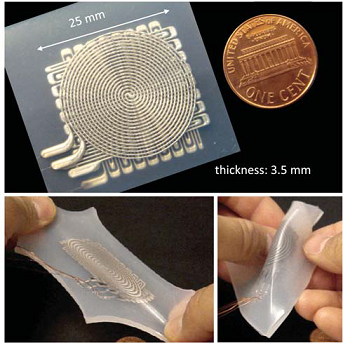
\includegraphics[width=0.9\linewidth]{img/precyzyjna_prezentacja.png} 
    \caption{Prezentacja wykonanego prototypu sztucznej skóry} 
  \end{subfigure}%%
  \begin{subfigure}[t]{0.495\linewidth}
    \centering
    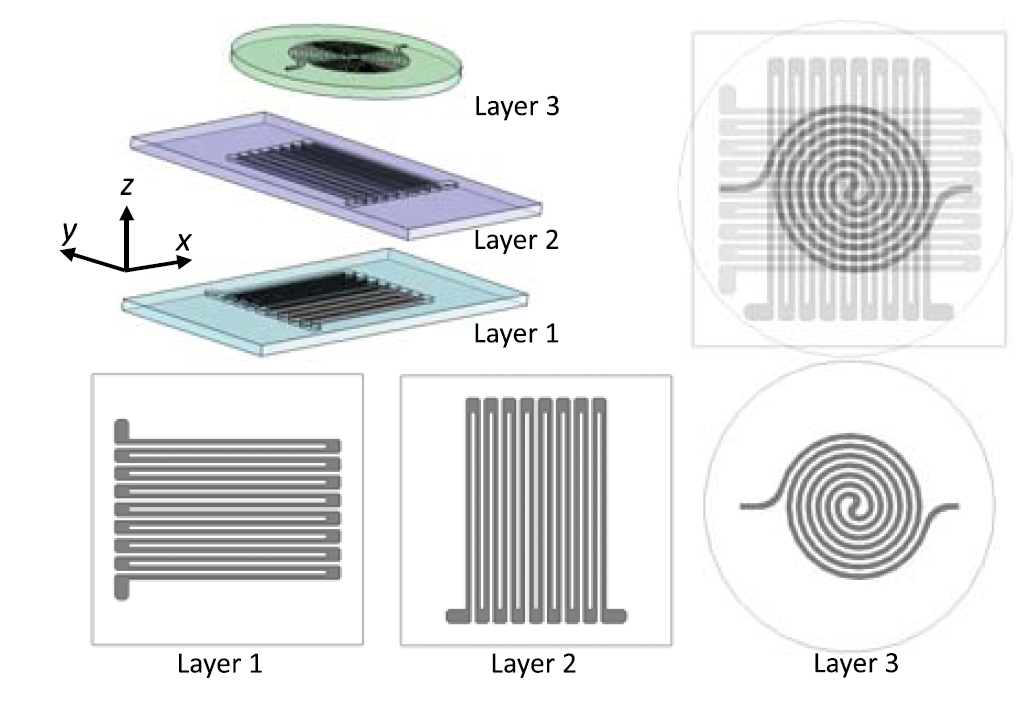
\includegraphics[width=0.95\linewidth]{img/przekroj_precyzyjna.png}
    \caption{Schemat budowy i ułożenia kolejnych warstw czujnika} 
  \end{subfigure}
  \centering
  \caption{Prezentacja i schemat budowy sztucznej skóry z wbudowanymi mikrokanałami \cite{b_article_tactile_precise}}
  \label{f_przeglad_prezyzyjna}
\end{figure}

Podstawowa zasada działania czujnika polega na pomiarze rezystancji poszczególnych kanałów. Mierzona rezystancja wzrasta jeśli kanaliki wypełnione przewodnikiem są rozciągane. Jest to związane ze zmniejszającym się przekrojem kanałów oraz jednocześnie rosnącą ich długością. 
Rezystancja mierzona jest przez pomiar spadku napięcia na poszczególnych warstwach. Zmierzony sygnał jest kolejno wzmacniany i wysyłany na przetworniki analogowo-cyfrowe. Stamtąd jest wysyłany do mikrokontrolera, który może przesłać dane dalej do systemu \cite{b_article_tactile_precise}.
% Doświadczalnie stwierdzono, że czujnik może być rozciągany o $250\%$ bez problemów w pomiarach. Jego rezystancja waha się wtedy od $\sim 2,5 \Omega$ przy braku nacisku do kilkunastu ($\sim12 \Omega$) przy rozciągnięciu o $100\%$. Pomiary są bardzo powtarzalne, ale zawierają histerezę oraz są zależne od szybkości zwiększania przykładanego nacisku 

Opisywany czujnik jest dopiero na początkowym etapie badań i nie posiadał jeszcze dokładnie sprecyzowanego zastosowania. Ze względu na jego budowę i możliwość dopasowania kształtu można go stosować w miejscach o nietypowym kształcie lub małym rozmiarze i przekroju. Sam czujnik może zostać także bardziej zminiaturyzowany lub posiadać inne ułożenie kanalików, które dadzą mu inne możliwości pomiaru napięć.

\newpage
\section{Wykorzystane narzędzia}
\label{s_narzedzia}

\subsection{Mikrokontroler kontrolujący sztuczną skórę - STM32}

Wybór odpowiedniego mikrokontrolera jest najprawdopodobniej najważniejszym zadaniem jeśli chodzi dalszy kierunek prowadzonych prac w zakresie wykonania sterownika sztucznej skóry. Wybrany model musi przede wszystkim spełniać swoje zadanie obsługi sztucznej skóry. Od jego wyboru zależy pozostała część komponentów elektronicznych, które muszą zostać dobrane tak, aby były kompatybilne z mikrokontrolerem. 
Od mikrokontrolera zależy także wybór narzędzi do jego programowania, ponieważ nie wszystkie środowiska programistyczne wspierają programowanie wszystkich układów.

Wybrany przeze mnie mikrokontroler należy do rodziny STM32 od ST Microelectronics. Mikrokontrolery STM32 są mikrokontrolerami 32-bitowymi z architekturą procesora Arm\textsuperscript{\textregistered}Cortex\textsuperscript{\textregistered}-M. Mikrokontrolery te oferują dużą wydajność, pracę w układach czasu rzeczywistego, wewnętrzne przetworniki sygnału analogowego oraz niski pobór mocy w~jednym układzie \cite{b_site_STM32}. Mikrokontrolery z~rodziny STM32 występują w~kilku seriach, z~których każda oferuje inne cechy kluczowe. W~każdej z~tych serii znajduje się również wiele modeli w różnych wariantach produkcji. Mnogość opcji doboru mikrokontrolera sprawia, że każdy może dobrać model właściwie dobrany do potrzeb realizowanego projektu. Na~rysunku \ref{f_przekroj_stm} zostały przedstawione serie mikrokontrolerów oferowanych przez ST i ich potencjalne zastosowanie.

\begin{figure}[!h]
    \centering 
    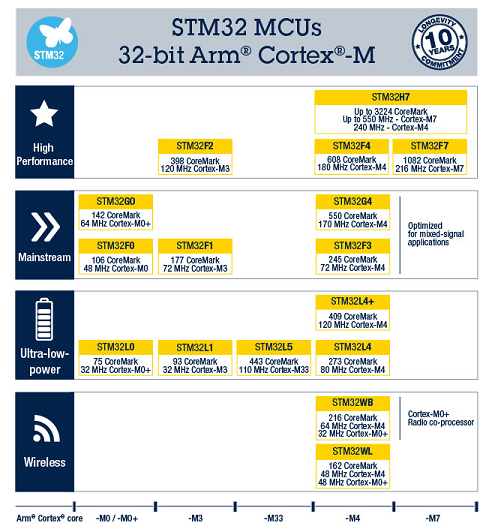
\includegraphics[width=0.7\linewidth]{img/przekroj_stm.png}
    \caption{Przekrój zastosowań mikrokontrolerów z rodziny STM32 \cite{b_site_STM32}}
    \label{f_przekroj_stm}
\end{figure}

Mikrokontrolery oferowane przez ST są szeroko wykorzystywane w zastosowaniach zarówno hobbystycznych, komercyjnych, jak i specjalistycznych. Posiadają duże wsparcie producenta, jak również wiele dedykowanych, stale rozwijanych i darmowych narzędzi ułatwiających pracę z nimi. Dokumentacja jest bardzo przejrzysta oraz ogólnodostępna na stronie producenta, zawiera pełny opis dostępnych peryferiów oraz ich specyfikację. Większość układów wspiera także FreeRTOS, co umożliwia wygodne użycie ich w~systemach czasu rzeczywistego.

Firma ST oferuje także płytki rozwoje z serii Nucleo i Discovery. Są one idealne jako pierwszy etap rozwoju projektu, ponieważ pozwalają korzystać z zalet mikrokontrolera zanim powstanie płytka drukowana, na której zostanie on umieszczony. Płytki rozwojowe pozwalają w ten sposób rozwijać projekt bez nadmiernych początkowych kosztów. Przykładem wykorzystania takiej płytki rozwojowej jest otrzymany przeze mnie prototyp sztucznej skóry widoczny na rysunku \ref{f_otrzymany_prototyp}, gdzie jako płytka rozwojowa zostało użyte Nucleo-F767ZI \cite{b_report_otrzymane}.
Dodatkowo narzędzia oferowane przez ST pozwalają przenosić napisany wcześniej kod na mikrokontrolery z innych serii co ułatwia przeniesienie pracy wykonanej na płytce rozwojowej na gotowy prototyp.

W kolejnych podrozdziałach zostały omówione niektóre z oferowanych przez ST narzędzi oraz szerokie wsparcie dla środowisk programistycznych, nie tylko tych promowanych przez ST. Narzędzia te pozwalają na dużo łatwiejszą pracę z mikrokontrolerem.

\subsubsection{Biblioteka HAL}
Jednym z narzędzi ułatwiających pracę była wykorzystana przeze mnie biblioteka HAL. Biblioteka ta jest oficjalnie dystrybuowana przez ST jako podstawowa biblioteka umożliwiająca i ułatwiająca programowanie mikrokontrolerów STM32. W praktyce biblioteka ta jest wysokopoziomowym interfejsem do części sprzętowej mikrokontrolera, pozwalając programiście w łatwy i przystępny sposób programować mikrokontroler.
Należy jednak pamiętać, że biblioteka wysokopoziomowa HAL poświęca jednak część wydajności i~szybkości działania mikrokontrolera na rzecz łatwości programowania i uniwersalności napisanego kodu.

Biblioteka HAL pozwala użytkownikowi także na wygodne przenoszenie kodu pomiędzy mikrokontrolerami z różnych rodzin STM32. Wygodne przenoszenie kodu pozwala na zmianę mikrokontrolera nawet na zaawansowanym etapie pracy, kiedy okaże się, że~obecna konfiguracja jest niewystarczająca. 
Jest to możliwe dzięki implementacji publicznych funkcji wykorzystywanych przez użytkownika w sposób dedykowany dla danego mikrokontrolera, przy czym z perspektywy użytkownika sposób wywołania funkcji (nazwa, parametry wywołania) się nie zmieniają. Takie podejście jest głównym powodem, dla którego napisany program sterownika sztucznej skóry korzystał z tej biblioteki.

\subsubsection{Narzędzie STM32CubeMX}
STM32CubeMX jest bardzo przydatnym narzędziem dystrybuowanym oficjalnie przez ST Microelectronics. Na etapie projektowania systemu, w szczególności części elektronicznej, pozwala na ułatwienie doboru odpowiedniego mikrokontrolera i przypisanie pinów mikrokontrolera do pracy z dobranymi układami. Na etapie programowania rozwiązanie umożliwia wygodną konfigurację używanego mikrokontrolera oraz wstępne wygenerowanie kodu poprawnie inicjującego wszystkie niezbędne do pracy peryferia.

Dobór mikrokontrolera polega na wybraniu najlepszego układu do danego rozwiązania. Nie jest to łatwe, ponieważ na rynku jest nawet po kilkaset różnych konfiguracji mikrokontrolerów od wielu producentów. Dlatego wiele firm, w tym ST, udostępnia narzędzie do wyboru odpowiedniego układu, poprzez filtrowanie całej bazy na podstawie wprowadzonych wymaganych parametrów. Takie narzędzie filtrowania zostało zaimplementowane właśnie w narzędziu STM32CubeMX. Wymogi w moim przypadku nie były bardzo ograniczające, więc mój wybór padł na prosty i tani mikrokontroler STM32F103RB, którego wcześniej już używałem w innych projektach. Ekran doboru mikrokontrolera jest widoczny na rysunku \ref{f_cube_micro}.

\begin{figure}[!h]
    \centering
    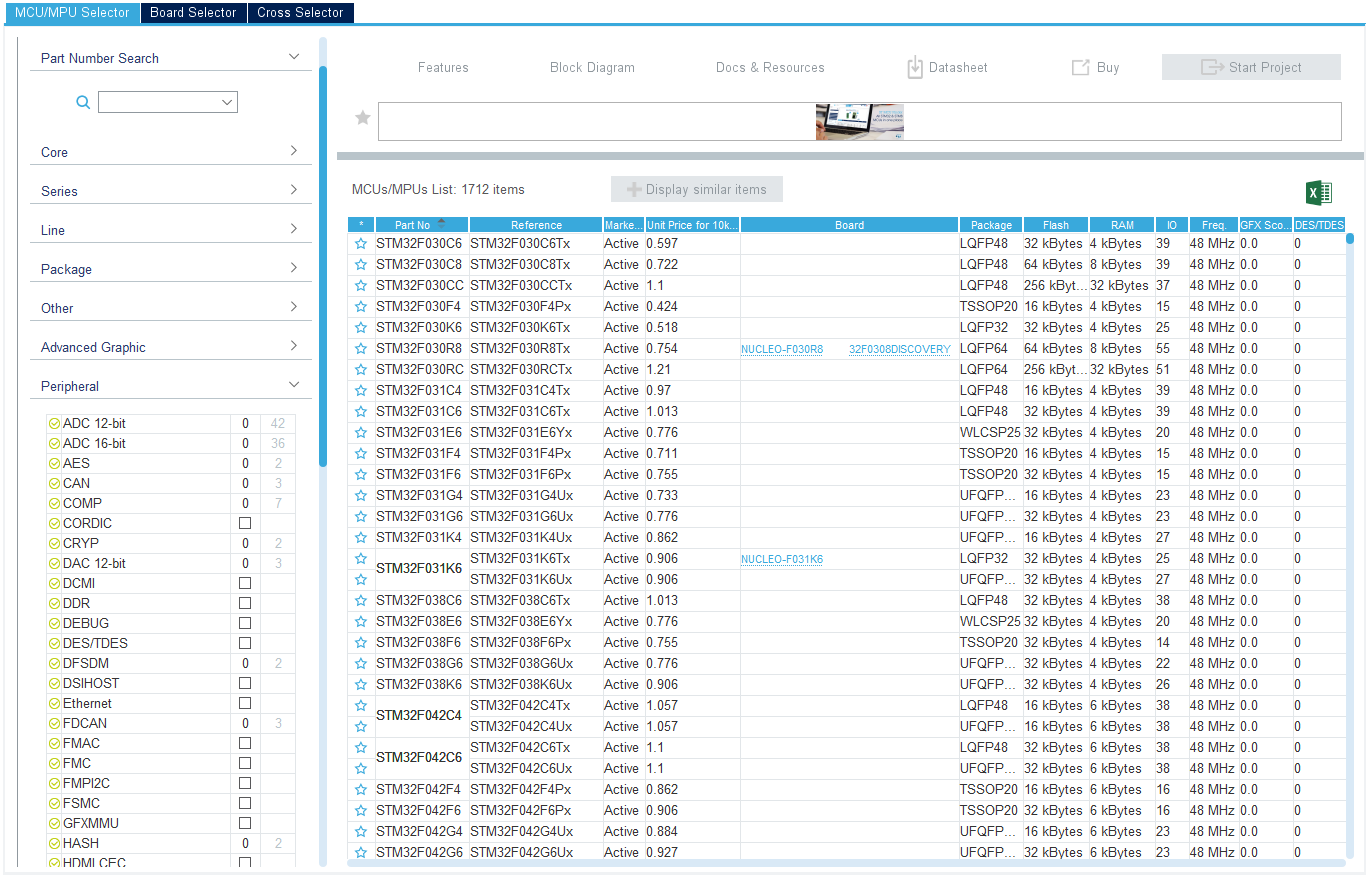
\includegraphics[width=0.95\linewidth]{img/cube_mcu_select.png} 
    \caption{Okno wyboru mikrokontrolera programu STM32CubeMX} 
    \label{f_cube_micro}
\end{figure}

Po wyborze odpowiedniego mikrokontrolera narzędzie przechodzi do widoku konfiguracji peryferiów. Widok ten przedstawia podgląd mikrokontrolera i wyprowadzonych z niego pinów wraz z oznaczeniem ich przeznaczenia i tego, czy są używane czy wolne. Na tym etapie można skonfigurować wybrane peryferia, a program automatycznie zarezerwuje potrzebne do tego piny i odświeży podgląd mikrokontrolera. W przypadku wystąpienia konfliktu lub braku możliwości użycia danego peryferium program nie pozwoli nam go skonfigurować. Narzędzie umożliwia także ręczną konfigurację pinów mikrokontrolera lub przenoszenie miejsca wyprowadzenia danego peryferium spośród możliwości oferowanych przez mikrokontroler.

Rozwiązanie z podglądem wyjść pinów mikrokontrolera jest bardzo przydatne na~etapie projektowania obwodu drukowanego do obsługi mikrokontrolera. Pozwala już na dość wczesnym etapie zaplanować wygląd i kształt takiej płytki. Taki widok pozwala także zaplanować, które wyjścia mikrokontrolera użyć, aby jak najmniejszym kosztem poprowadzić połączenia do dalszych komponentów na płytce. Bazując na własnym doświadczeniu, takie podejście znacznie zmniejsza możliwość wystąpienia błędu w porównaniu do metody alternatywnej planowania wyprowadzeń, czyli samej dokumentacji. Dokumentacja również zawiera wszystkie potrzebne informacje, lecz jej forma (tekst i~tabele) nie jest w stanie wykryć wykonanych przez projektanta błędów. CubeMX pozwala dodatkowo na wygodne ustawianie częstotliwości taktowania poszczególnych peryferiów. Podczas doboru częstotliwości taktowania obliczane i korygowane są częstotliwości taktowania innych peryferiów zależne od tej modyfikowanej przez użytkownika. Pozwala to na~znaczne zmniejszenie ilości błędów związanych z błędną częstotliwością taktowania na poszczególnych peryferiach. Wygląd programu w oknie konfiguracji mikrokontrolera został przestawiony na rysunku \ref{f_cube_konf}.

\begin{figure}[!h]
    \centering
    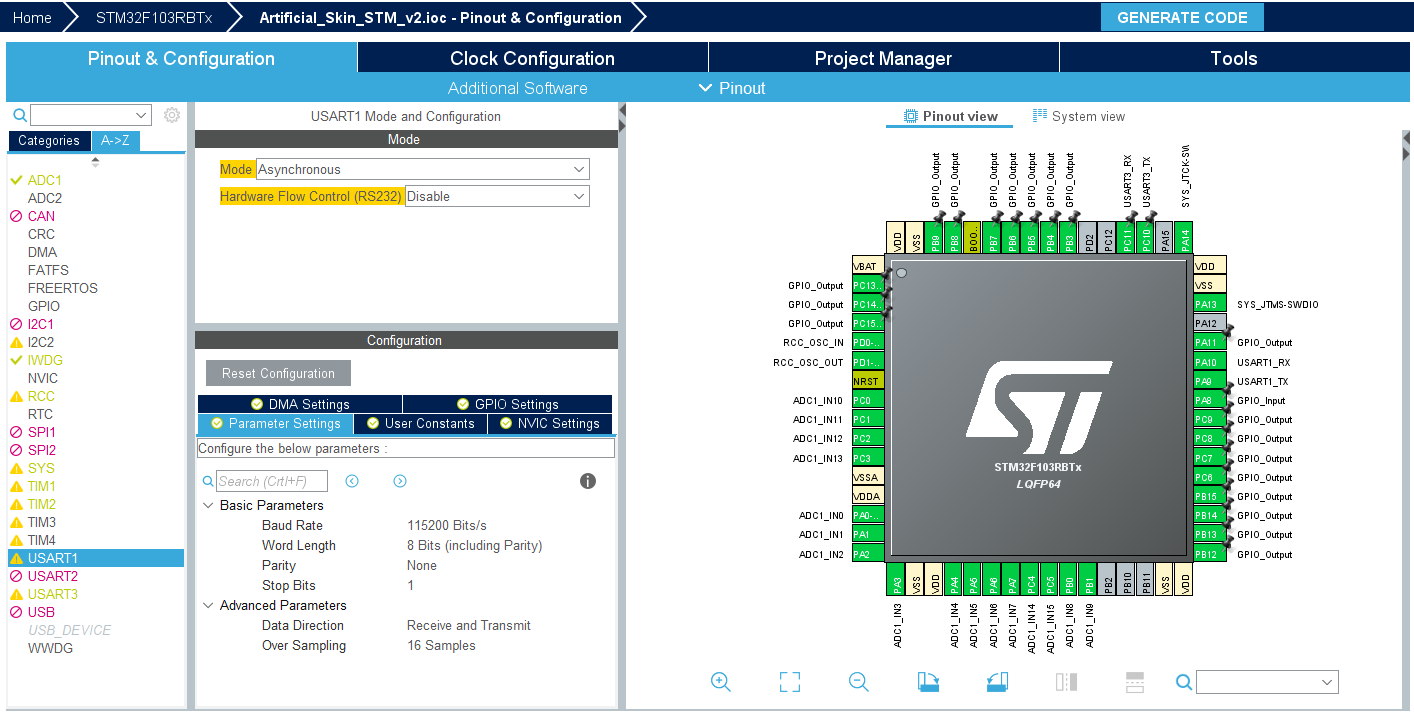
\includegraphics[width=0.95\linewidth]{img/cube_config.png}
    \caption{Okno konfiguracji mikrokontrolera programu STM32CubeMX} 

  \label{f_cube_konf}
\end{figure}

Ostatnią, ale nie mniej ważną funkcją tego narzędzia jest generowanie kodu źródłowego programu. Wygenerowany kod źródłowy jest od razu gotowy do skompilowania i działania. Co prawda taki kod jeszcze nie wykonuje oczekiwanego przez programistę zadania, ale pozwala na ominięcie żmudnej pracy uruchamiania wszystkich peryferiów ręcznie. Wygenerowany kod jest logicznie podzielony na pliki w zależności od peryferium. Niestety jest on również nieprzejrzysty, więc jego uporządkowanie wymaga od programisty trochę pracy \cite{b_site_cube}.

\subsubsection{Środowisko programistyczne CLion}
Po wygenerowaniu wstępnego kodu źródłowego potrzebne jest jego uzupełnienie o~zaplanowane funkcje. Na rynku do wyboru jest wiele różnych środowisk programistycznych, ale mój wybór padł na środowisko, które wspiera programowanie mikrokontrolerów STM32. Wybrane zostało środowisko oferowane przez JetBrains - CLion, które od wersji 2019.1 oficjalnie posiada dedykowane wsparcie dla mikrokontrolerów z~rodziny STM32 \cite{b_site_CLion_STM_support}. Wcześniejsze wersje oprogramowania wspierały tylko z wykorzystaniem odpowiednich dodatkowo instalowanych wtyczek \cite{b_site_CLion_STM_support_v2}. % Co działało dużo lepiej, ale już chuj z tym
Wsparcie środowiska dla systemów STM32 objawia się przede wszystkim poprzez wbudowaną funkcję do generacji pliku \textit{CMakeLists.txt} niezbędnego, aby w środowisku CLion poprawnie skompilować projekt. Generacja tego pliku jest opierana na wygenerowanych wcześniej przez program STM32CubeMX plikach, zawierających wszystkie informacje o docelowym mikrokontrolerze.
Wspierany jest także zautomatyzowany wybór mikrokontrolera docelowego, na który program będzie wgrywany, spośród dostępnych w bibliotekach list. Po wykonaniu tych dwóch kroków środowisko jest skonfigurowane i gotowe do kompilacji oraz wgrywania programu na mikrokontroler \cite{b_site_CLion_STM_support}.

Środowisko CLion wspiera także debugowanie napisanych programów i nie potrzebuje do tego specjalistycznych urządzeń dostarczanych przez ST. Do debugowania (jak również zwykłego programowania) wystarczy posiadać konwerter na interfejs SWD. Debugowanie mikrokontrolerów, podobnie jak zwykłych programów, polega na zatrzymaniu programu po osiągnięciu oznaczonego miejsca w kodzie programu i zatrzymaniu programu w tym miejscu. Po zatrzymaniu można przeglądać jakie program przyjmuje wartości dla użytych zmiennych lub samemu nadawać tym zmiennym wartości. Debugowanie mikrokontrolerów różni się od debugowania zwykłych programów tym, że mikrokontroler jest w~stanie pracować na przerwaniach. W kodzie programu objawia się to faktem używania funkcji, do których kod nie ma odniesień. Należy to mieć na uwadze, ponieważ pomiędzy podglądaniem zmiennych program może zmieniać ich wartości właśnie w przerwaniach bez naszej wiedzy. 
Ograniczenia jakie występują w środowisku polegają na tym, że CLion nie pozwala na debugowanie z oznaczeniem wielu miejsc w kodzie, w których program się zatrzyma.

Opisane w powyższych akapitach cechy zawiera praktycznie każde środowisko przystosowane do programowania mikrokontrolerów. To, w czym CLion zdobywa przewagę nad innymi środowiskami to wygoda użytkowania. Na tę wygodę składają się między innymi: ciemny motyw (nie każde środowisko taki posiada% tak o tobie myślę Eclipse
), intuicyjny interfejs, duża dowolność w konfiguracji środowiska. Program posiada także sporo skrótów klawiaturowych przyspieszających pracę oraz inne przydatne funkcjonalności jak np. zakładki do konkretnych miejsc w kodzie. Z tych właśnie powodów, i częściowo z przyzwyczajenia do środowiska, mój wybór padł właśnie na CLiona.

% STMStudio, StLinkUtility??

% Opisywać Altiuma?

% \subsection{Obsługa portów komunikacyjnych - PuTTY}
% Jak mi się będzie nudziło to napiszę to jako zapychacz

\subsection{Środowisko pracy - ROS}

System ROS (Robot Operating System) jest potężnym i elastycznym środowiskiem pozwalającym na tworzenie i testowanie oprogramowania robotów. Zawiera wiele narzędzi i bibliotek dostosowanych specjalnie do pracy w tak specjalistycznym jak robotyka zakresie. ROS jest również systemem pozwalającym na połączenie różnych modułów percepcyjnych i aktuatorów w jednym systemie \cite{b_site_ROS}.

ROS jest strukturalnie podzielony na węzły odpowiadające uruchomionym procesom, tematy odpowiadające kanałom przesyłania danych, usługi będące węzłami wykonującymi pojedyncze akcje oraz serwery parametrów przechowujących informacje, które nie zmieniają się zbyt często. Jeden węzeł może wysyłać i odbierać na wielu tematach, podobnie jak na jeden temat może nadawać wiele węzłów. Tematy mogą być także pogrupowane w zależności od tego, z jakiem pakietem są związane. Cała ta nieskomplikowana w założeniach struktura jest otwarta na modyfikacje i rozbudowę poprzez dodawanie kolejnych węzłów \cite{b_site_ROS_wiki}.

Narzędzia udostępniane przez ROS są bardzo pomocne w pracach, szczególnie na~etapie testowania rozwiązań i szukania błędów w implementacji. Dostępnych narzędzi jest wiele, ale jednym z najważniejszych jest RVIZ. RVIZ jest narzędziem służącym do wizualizacji aktualnego stanu robota w przestrzeni trójwymiarowej. Nie jest to jednak symulator, ponieważ potrafi on pokazywać tylko informacje znane robotowi, które może on odczytać wykorzystując zamocowane na nim czujniki lub kamery. Widoczne są także informacje zapisane wcześniej do pamięci robota, takie jak mapa terenu \cite{b_site_ROS_tools}. Widok narzędzia RVIZ z odwzorowaną mapą laboratorium został przedstawiony na rysunku \ref{f_ros_tools_rviz}.

\begin{figure}[!h]
    \centering
    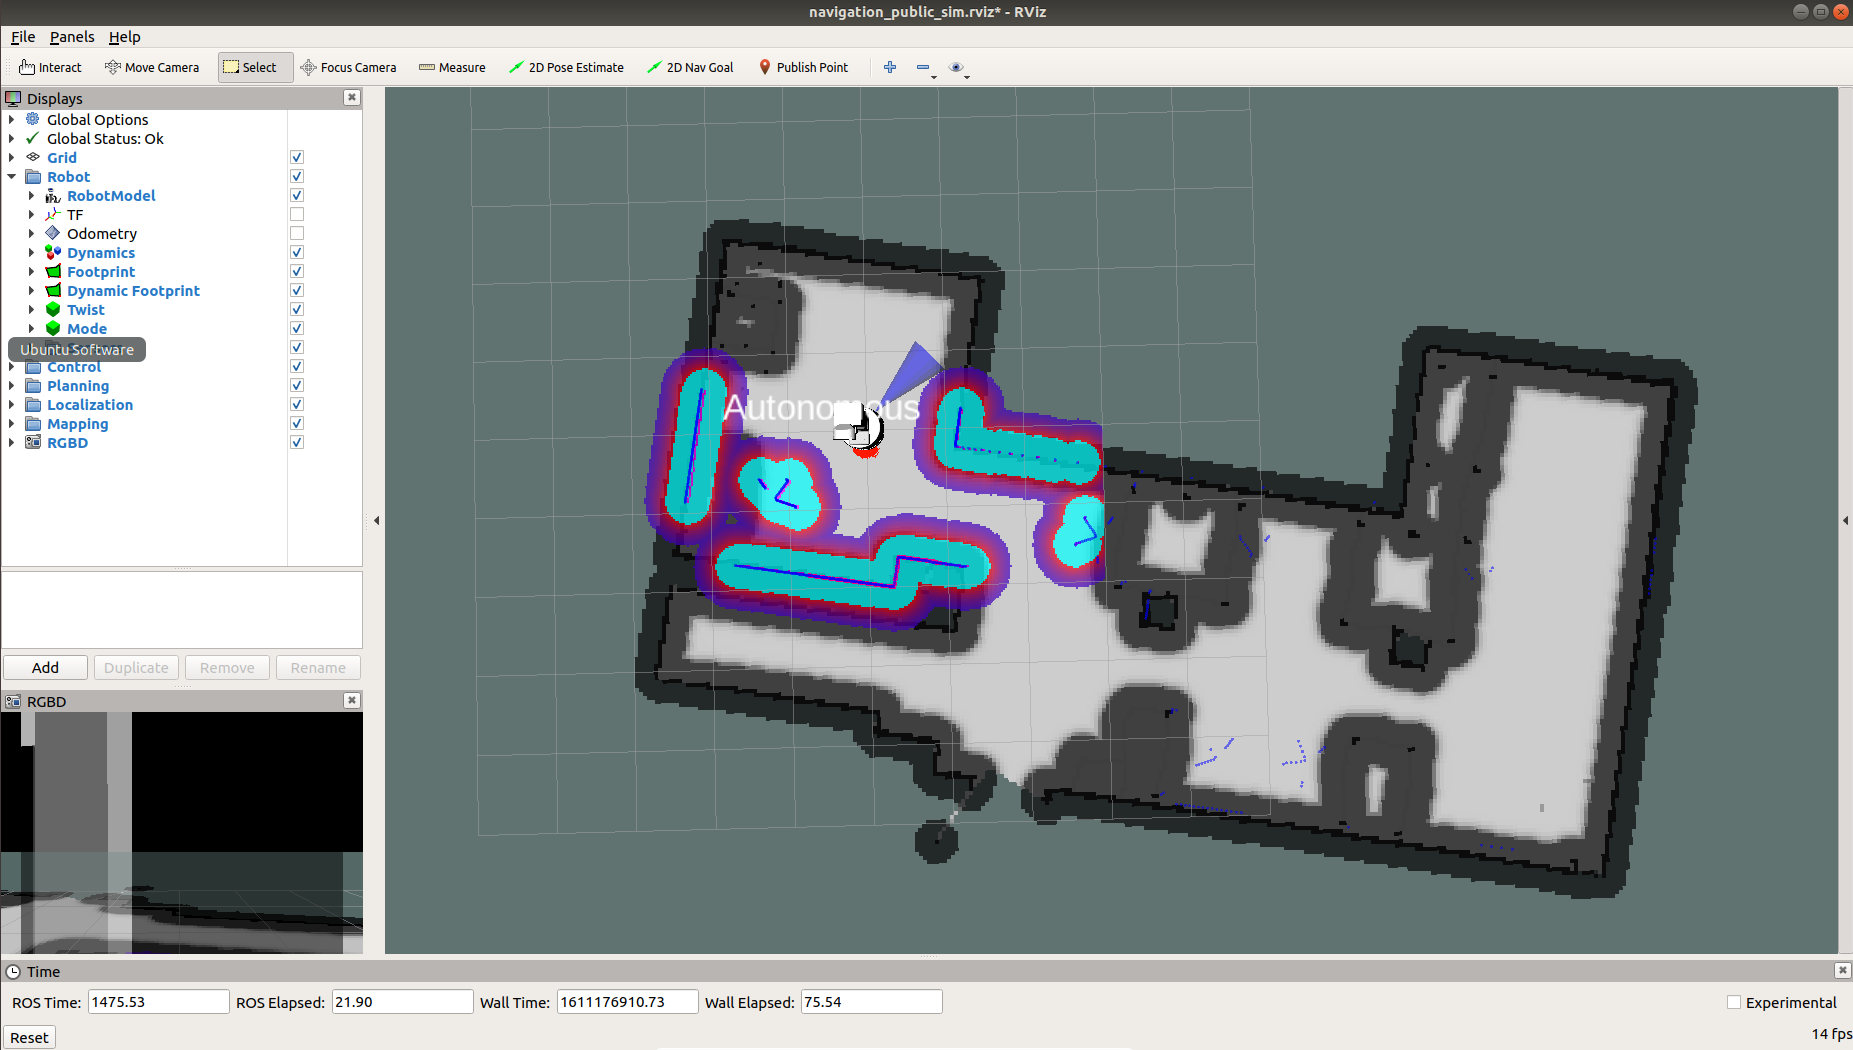
\includegraphics[width=0.95\linewidth]{img/ros_tools_rviz.png} 
    \caption{Narzędzie RVIZ \cite{b_site_ROS_tools}} 
     \label{f_ros_tools_rviz}
    % \vspace{4ex}
    \end{figure}

Kolejnym narzędziem znacząco pomagającym w podglądzie aktualnego stanu robota jest rqt\_graph. Rqt\_graph wizualizuje aktualny stan robota pokazując strukturę węzłów i~tematy, które znajdują się w całej strukturze systemu. Narzędzie to wizualizuje strukturę przedstawiając ją w formie grafu skierowanego. Udostępnione są też dodatkowe funkcje odfiltrowania niektórych danych, np. węzłów, które nie publikują danych i nie wpływają w żaden sposób na pracę systemu \cite{b_site_ROS_tools}. Przykładowy widok narzędzia rqt\_graph jest widoczny na rysunku \ref{f_ros_tools_rqt}.


    \begin{figure}[!h]
    
    \centering
    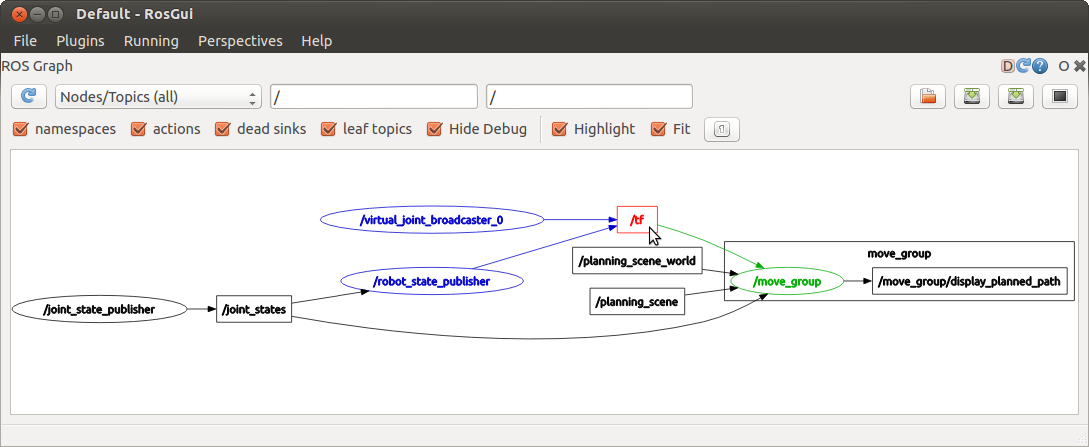
\includegraphics[width=0.95\linewidth]{img/ros_tools_rqt.png}
    \caption{Narzędzie Rqt\_graph \cite{b_site_ROS_tools}} 
     \label{f_ros_tools_rqt}
    % \vspace{4ex}

\end{figure}

% plot 

ROS oferuje także narzędzia opierające się głównie na komunikacji za pomocą konsoli, a jednym z częściej używanych jest rostopic. Rostopic daje duże możliwości w kontrolowaniu tematów (kanałów danych). Najczęściej wykorzystywana jest funkcja echo, która wyświetla na konsoli, w czasie rzeczywistym, wszystkie informacje, które są przesyłane danym strumieniem. Pozwala to na szybkie znajdowanie i naprawianie błędów, jeśli przesyłane są złe informacje lub w ogóle nie są przesyłane. Rostopic pozwala także na wysyłanie wiadomości na podany przez operatora temat. Dodatkowo umożliwia także otrzymywanie informacji o wszystkich dostępnych w systemie tematach i typie informacji na nich wysyłanych \cite{b_site_ROS_tools}.

Innymi przydatnymi narzędziami są rosbag oraz rqt\_bag pozwalające na zbieranie i~przeglądanie zebranych danych. Rosbag jest narzędziem przeznaczonym do zbierania danych przesyłanych na tematach oraz ich późniejszego odtworzenia, a nawet wysłanie z powrotem na temat. Rqt\_bag jest podobnym narzędziem do rosbag, ale posiada wbudowany interfejs użytkownika \cite{b_site_ROS_tools}.


\subsection{Platforma symulacyjna - Gazebo}
\label{ss_narzedzia_gazebo}
Ważną kwestią, jeśli chodzi o testowanie, jest przeprowadzenie wstępnych testów na symulacji. Używanie symulacji w testowaniu robotów jest ważne, aby w żaden sposób nie narażać człowieka, robota ani środowiska na jakiekolwiek niebezpieczeństwa. 
Symulator dostępny jest także lokalnie na komputerze bez potrzeby prowadzenia testów w laboratorium, co znacznie ułatwiło mi testy szczególnie w czasie pandemii. 
Finalnie jednak w ten sposób nie można sprawdzić działania prototypu w rzeczywistych warunkach i~zweryfikować czy współpracuje on z fizycznym robotem.

Środowisko symulacyjne doskonale sprawdziło się natomiast do celów weryfikacji wybranych i zaimplementowanych algorytmów sterowania robotem. Można sprawdzić czy robot się prawidłowo zachowuje i reaguje na wysyłane sygnały.
W niniejszym przypadku symulacja pozwoliła także w wygodny sposób skonfigurować dołączany do systemu węzeł bez ryzyka uszkodzenia sprzętu. Sprawdzona została także poprawność działania zaprojektowanej sztucznej skóry i sprawność komunikacji sterownika z komputerem.

W kwestii symulatora wybór padł na program Gazebo, który jest bardzo dobrze przystosowany do integracji z systemem ROS i był projektowany z myślą o testowaniu robotów. Gazebo posiada bardzo wygodny interfejs, dobrą fizykę i pozwala użytkownikowi na bardzo dużą swobodę w projektowaniu jego elementów. Gazebo wspiera także dużą liczbę różnych czujników, efektorów i innych podzespołów, jak również roboty funkcjonujące na rynku \cite{b_site_Gazebo}.

Dla ułatwienia testów wykorzystane zostały istniejące i wykonane wcześniej przez zespół laboratoryjny pakiety: świata, który był dobrym odwzorowaniem faktycznego laboratorium oraz robota. Odwzorowanie robota było oparte na pakiecie, który udostępnia firma go produkująca - PAL Robotics. Pozwoliło mi to na testy w praktycznie tym samym środowisku, co prowadzone później testy fizyczne.

\subsection{Platforma testowa - robot Tiago}

Robot Tiago jest produkowany przez hiszpańską firmę PAL Robotics, która ma w~swoim portfolio jeszcze kilka robotów do innych zastosowań (w tym przemysłowych). Zaprojektowany przez nich robot Tiago jest typowym robotem asystującym mającym za zadanie współpracować z ludźmi w ich domowym środowisku i wykonywać zlecone mu zadania \cite{b_site_tiago}.

Tiago jest robotem modułowym, co znaczy że można dopasowywać jego możliwości i zainstalowane podzespoły do własnych potrzeb. Jako podstawa oferowana jest baza jezdna z komputerem, czujnikami odległości oraz kamerą stereo. Jako dodatkowe opcje można wybrać manipulatory o siedmiu stopniach swobody, ich chwytaki, dodatkowy osprzęt (kamery, tablet), czy też wydajniejsze podzespoły wewnętrzne robota \cite{b_site_tiago}. Sam robot został przedstawiony na rysunku \ref{f_tiago_zwykly}.

Robot wyposażony jest przede wszystkim w układ sterowania wykorzystujący możliwości procesorów Intel\textsuperscript{\textregistered}Core\texttrademark i5 lub i7, co zapewnia mu dużą moc obliczeniową. Każda wersja posiada także laserowy czujnik odległości zamontowany z przodu w podstawie robota. Czujnik laserowy ma zasięg zależnie od wersji od $5,6m$ do $25m$ zasięgu i pole widzenia $\ang{220}$. U podstawy znajduje się napęd w standardowej konfiguracji układu różnicowego, czyli dwa koła niezależnie napędzane oraz kilka swobodnych, służących przede wszystkim jako punkty podparcia. W górnej części robota, która przypomina głowę, umieszczona została kamera stereowizyjna, która pozwala na wykorzystywanie na robocie zaawansowanych algorytmów przetwarzania obrazu. Niedaleko znajduje się także mikrofon rejestrujący dźwięki z otoczenia. Cała górna część umieszczona została na podnoszonym i~opuszczanym przez robota tułowiu. Robot posiada także wbudowaną komunikację WiFi, co umożliwia w pełni bezprzewodowe sterowanie nim, również przez Internet. Komunikacja ta upraszcza również użycie robota w coraz bardziej popularnych systemach IOT \cite{b_site_tiago}.

PAL Robotics udostępnia także za darmo poradniki jak używać ich robota i modelu ich robota w systemie ROS. Oferują oni pełne wsparcie opisanych wcześniej rozwiązań co znacznie ułatwia wstępne testowanie kodu, nawet bez dostępu do samego robota. Oferowane przez nich narzędzia posiadają także funkcję dostosowywania osprzętu robota według własnych upodobań \cite{b_site_tiago, b_site_tiago_ROS}.

\newpage
\section{Budowa sztucznej skóry}
\label{s_budowa}

\subsection{Otrzymany prototyp i stan badań}

Otrzymane w ramach pracy materiały związane z prototypem składały się z:
\begin{itemize}
    \item prototypu czujnika o rozmiarze $4x4$ pola i wymiarach $40x40 cm$ (rysunek \ref{f_otrzymany_prototyp}),
    \item układu elektronicznego obsługującego prototyp i komunikującego się z komputerem,
    \item wersji otwartej programu wgranego na mikrokontroler,
    \item oprogramowania w języku Python obrazującego odczyty napięcia ze sztucznej skóry ( rysunek \ref{f_otrzymany_apka}),
    \item dokumentacji zawierającej wykonane badania i opis budowy prototypu.
\end{itemize}

Otrzymany prototyp był zbudowany z dwóch fragmentów gumy typu NBR190 o wymiarach $40x40 cm$ i grubości $10 mm$ służących jako warstwy nośne, absorbujące uderzenia i rozkładające nacisk. Wewnątrz, na każdej z gum, zostały naklejone równolegle 4 paski taśmy miedzianej o szerokości $50 mm$ mające za zadanie przewodzić sygnały elektryczne. Taśma miedziana została naklejona na gumach w taki sposób, aby po ich złożeniu tworzyć matrycę przecięć o rozmiarze $4x4$. Do końcówek taśmy miedzianej z jednej strony zostały przylutowane przewody, które zostały dalej wyprowadzone na płytkę stykową. Pomiędzy warstwami gumy została umieszczona pojedyncza warstwa folii Velostat o wymiarach $30x30 cm$. Wszystkie elementy wewnętrzne zostały zabezpieczone przed przesuwaniem przez przyklejenie ich taśmą izolacyjną do powierzchni gumy. Obie warstwy gumy zostały ze sobą złączone trzema śrubami z użyciem szerokich podkładek, aby nie deformować nadmiernie gumy, oraz z użyciem nakrętek motylkowych, aby ułatwić późniejsze składanie i rozbieranie prototypu. Czwarty róg pozostał nieskręcony śrubą i~w~ten sposób umożliwiał w razie potrzeby na szybkie spojrzenie do wnętrza prototypu. Otrzymany prototyp wraz z~częścią elektroniczną znajduje się na rysunku \ref{f_otrzymany_prototyp} \cite{b_report_otrzymane}.

\begin{figure}[!h]
    \centering 
    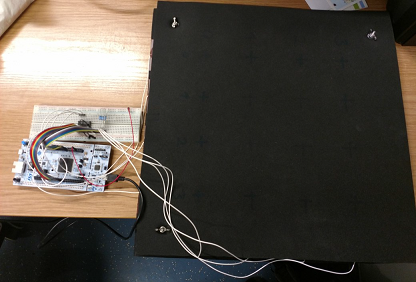
\includegraphics[width=0.95\linewidth]{img/otrzymane_prototyp.png}
    \caption{Otrzymany prototyp sztucznej skóry \cite{b_report_otrzymane}}
    \label{f_otrzymany_prototyp}
\end{figure}

Część sterująca prototypu została skonstruowana na płytce rozwojowej Nucleo-F767ZI. Pozostała część układu elektrycznego została wykonana na płytce stykowej i w głównej mierze składała się z drabinki Darlingtonowej ULN2003A. Drabinka ta odpowiadała za przełączanie pomiędzy odczytami poszczególnych wierszy czujnika. Kolumny czujnika były podłączone bezpośrednio do mikrokontrolera STM32F767ZIT6U, do wbudowanych w~mikrokontroler przetworników analogowo-cyfrowych \cite{b_report_otrzymane}.

Program zapisany na mikrokontrolerze był bardzo prosty, a jego jedynym zadaniem było ciągłe przełączanie poszczególnych wierszy i kolumn oraz odczyt wartości dostępnych na pinach przetwornika analogowo-cyfrowego z częstotliwością około $\sim10 Hz$. Program, od~razu po wykonaniu odczytu, konwertował go ze stanu surowego na wartość odczytanego napięcia i taki odczyt wysyłał do komputera. Sygnał wysyłany był przez mikrokontroler interfejsem UART, a układ programatora ,instalowany fabrycznie na wszystkich płytkach z~serii Nucleo, przesyłał te dane dalej do komputera za pośrednictwem interfejsu USB \cite{b_report_otrzymane}.

Po stronie komputera zostało napisane oprogramowanie pozwalające na odczytywanie wiadomości wysyłanych przez mikrokontroler. Oprogramowanie napisano w Pythonie z~użyciem biblioteki PyQT i zaimplementowano mu prosty oraz intuicyjny interfejs. 
Wykonana aplikacja komputerowa przedstawiona jest na rysunku \ref{f_otrzymany_apka}.
Po lewej stronie znajduje się wizualizacja przyłożonej siły, gdzie każdy kwadrat odpowiada jednemu polu czujnika. Im większa siła została przyłożona do danego pola, tym jaśniejsze staje się pole na ekranie. Po prawej stronie interfejsu znajduje się natomiast wykres odczytanych wartości z~ostatnich kilkudziesięciu sekund z~jednego pola. Wykres przedstawia napięcie na polu sztucznej skóry w~zależności od czasu i~pozwala nie tylko odczytać dokładne wartości wykonanego pomiaru, ale~przede wszystkim jak ten pomiar się zmieniał.
Nad~wykresem znajdują się rozwijane listy pozwalające wybrać, pomiary którego czujnika chcemy aktualnie obserwować  \cite{b_report_otrzymane}.

\begin{figure}[!h]
    \centering 
    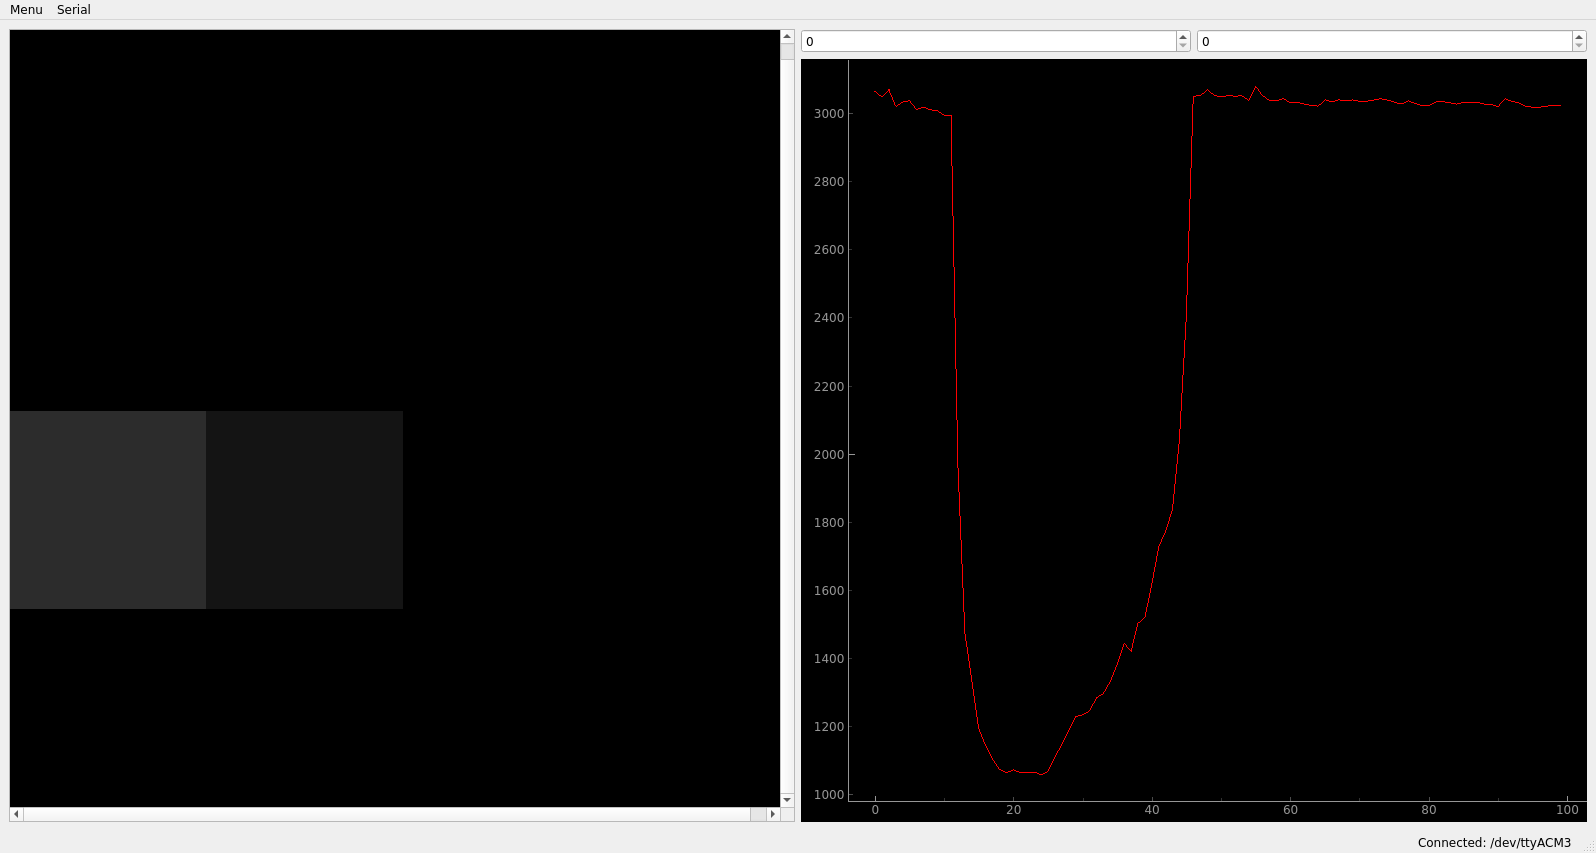
\includegraphics[width=0.95\linewidth]{img/otrzymane_apka.png}
    \caption{Otrzymana aplikacja odczytująca pomiary ze sztucznej skóry \cite{b_report_otrzymane}}
    \label{f_otrzymany_apka}
\end{figure}

Badania wykonane nad opisanym powyżej prototypem przebiegały głównie przed budową samego prototypu, a przedstawiony prototyp był ich zwieńczeniem. Prowadzone badania dotyczyły głównie wybrania odpowiednich rozwiązań i materiałów do budowy prototypu. Został wykonany przegląd literatury, którego efektem było ustalenie takiej budowy sztucznej skóry. Zostały ustalone założenia projektu oraz przystąpiono do wyboru materiałów. Jako materiał o zmiennej rezystancji została wybrana folia Velostat, a warstwy przewodzące folia miedziana. Aby dokonać wyboru najlepszego materiału nośnego zostały wykonane badania wielu (jedenastu) różnych rodzajów materiałów. Testowane one były pod kątem przewodności elektrycznej, trwałej odkształcalności i pochłanialności energii. Ostatecznie, jako materiał najlepiej spełniający postawione kryteria, wybrana została guma NBR190. Zwieńczeniem badań był opisywany wcześniej prototyp, na którym nie zostały wykonane żadne szczegółowe testy. Zostało tylko sprawdzone, czy rozwiązanie w ogólnym zakresie działa tak, jak było to przewidywane. Te nieskomplikowane testy przeszły pozytywnie \cite{b_report_otrzymane}.

Bazując na przekazanym prototypie zostały wyznaczone wszystkie obszary, w~których należy przeprowadzić dalsze prace. Zostały wyznaczone 4 główne warstwy: mechaniczna, elektroniczna, komunikacyjna i programowa. Dokonane wybory wraz z uzasadnieniem zostały przedstawione w rozdziałach: \ref{ss_budowa_mech}~-~warstwa mechaniczna (czujnik), \ref{ss_integracja_budowa}~-~warstwa mechaniczna (mocowanie do robota), \ref{ss_budowa_ele}~-~warstwa elektroniczna, \ref{ss_budowa_kom}~-~warstwa komunikacyjna, \ref{ss_budowa_prog}~-~warstwa programowa (część sterownika), \ref{ss_integracja_Python} oraz \ref{ss_integracja_algorytm}~-~warstwa programowa (część węzła w systemie ROS).
Schemat projektowanej sztucznej skóry, wraz z~wyszczególnieniem zakresów pracy przy poszczególnych warstwach został przedstawiony na rysunku~\ref{f_art_skin_system}.

\begin{figure}[!h]
    \centering 
    \includegraphics[width=0.95\linewidth]{img/art_skin_system.pdf}
    \caption{Schemat systemu sztucznej skóry wraz z wyszczególnionymi warstwami, przy których prowadzono prace}
    \label{f_art_skin_system}
\end{figure}

\subsection{Warstwa mechaniczna}
\label{ss_budowa_mech}

Część mechaniczna jest pierwszym elementem widocznym po spojrzeniu na sztuczną skórę. Jednak poza przystępnym wyglądem musi ona spełniać dużo bardziej podstawowe funkcje części mechanicznych. Przede wszystkim jest to szkielet całej konstrukcji, który trzyma całość w skupionej postaci oraz zapobiega przemieszczaniu się elementów czujnika. Jest ona także odpowiedzialna za ochronę przed uszkodzeniami pochodzącymi ze środowiska zewnętrznego. Bazując na tym spisana została lista założeń, które projektowana część mechaniczna musiała spełniać:
\begin{itemize}
    \item podatność i odporność mechaniczna - czujnik powinien móc się ugiąć oraz pochłonąć energię uderzenia, aby ochronić robota i otoczenie przed uszkodzeniem,
    \item możliwość stosowania na nierównych powierzchniach i na krzywiznach obudowy robota,
    \item niska masa, biorąc pod uwagę docelowe duże rozmiary czujnika,
    \item uniwersalność i skalowalność czujnika - możliwość stosowania w różnych konfiguracjach na różnych robotach.
\end{itemize}

Większość postawionych założeń dotyczących części mechanicznych jest spełniana przez użytą gumę mikroporowatą. Dlatego też to guma była dobierana do założeń projektowych tak, aby je spełniała.

Mechanicznie, budowa mojej wersji czujnika nie różniła się w dużej mierze od prototypu, który został mi przekazany jako podstawa prac. Czujnik również został zbudowany z~pięciu podstawowych warstw: mechanicznej zewnętrznej (guma), przewodzącej zewnętrznej (poziome paski folii miedzianej), folii Velostat, przewodzącej wewnętrznej (pionowe paski folii miedzianej) oraz mechanicznej wewnętrznej (guma). Jedynymi modyfikacjami wykonanymi w ramach pracy było dobranie doświadczalnie odpowiednich grubości gumy oraz rozbudowanie wewnętrznej warstwy nośnej czujnika o sztywny szkielet, będący łącznikiem pomiędzy giętkim czujnikiem, a obudową robota \cite{b_report_otrzymane}. Wykorzystana w~czujniku kolejność warstw została zobrazowana na rysunku \ref{f_otrzymany_budowa}.

\begin{figure}[!h]
    \centering 
    
\includegraphics[width=0.5\linewidth]{img/otrzymane_budowa.png}
    \caption{Przekrój budowy sztucznej skóry \cite{b_report_otrzymane}}
    \label{f_otrzymany_budowa}
\end{figure}

Aby utrzymać wszystkie warstwy złączone ze sobą nie zostały wykorzystane śruby, jak~w~poprzednim modelu, ponieważ one są bardzo kłopotliwe i nie zapewniają odpowiedniego zabezpieczenia, zarówno robota, jak i otoczenia. Jako materiał łączący warstwy ze sobą zostały użyte różnego rodzaju taśmy (montażowe, izolacyjne, dwustronne). Zapewniają one praktycznie niewidoczne połączenie pomiędzy warstwami i~nie wystają poza obręb zewnętrznej gumy. Najważniejszą ich zaletą jest jednak fakt, że nie wywierają one istotnych naprężeń w~warstwie gumy, co znacznie poprawia wyniki w~porównaniu z~wersją, gdzie czujnik jest skręcony śrubami.

\subsection{Warstwa elektroniczna}
\label{ss_budowa_ele}

Sterownik sztucznej skóry jest jedną z pierwszych warstw (zaraz za warstwą fizyczną czujnika), która odpowiada za poprawne działanie całego systemu. Informacje przez niego odczytywane są przesyłane bezpośrednio do systemu sterowania robotem. Z tego powodu jest to bardzo ważne, aby ta część działała prawidłowo i niezawodnie. Potencjalne złe działanie sterownika sztucznej skóry może skutkować wysyłaniem do komputera całkowicie nieprawdziwych informacji, a co za tym idzie działanie całego robota będzie nieprzewidywalne, wręcz niebezpieczne.

Warto zauważyć, że w tym projekcie jest to ostatnie miejsce, gdzie sygnał występuje jeszcze w formie analogowej - odczyty z poszczególnych pól czujnika są analogowe. Dane wysyłane z czujnika są już natomiast wysyłane przez magistralę USB w formie cyfrowej. Z~tego powodu ważne jest, aby na tym etapie wyeliminować możliwie dużo zakłóceń, które są przyczyną występowania błędów na sygnałach analogowych.

Zastosowany do tego zadania sterownik musi spełniać szereg różnych zadań, spośród których najważniejsze są:
\begin{itemize}
    \item obsługa wszystkich pól sztucznej skóry, poprzez odpowiednie doprowadzenie zasilania i odczyt wartości nacisku na pole,
    \item zapewnienie ciągłości i poprawności wykonywanych pomiarów,
    \item agregowanie pomiarów ze wszystkich pól i przesyłanie ich do jednostki sterującej w~formie łatwiejszej do dalszej obsługi,
    \item automatyczny reset w przypadku błędów krytycznych lub zawieszenia się systemu,
    \item szybka i stabilna komunikacja z komputerem nadrzędnym z wykorzystaniem standardowego łącza komunikacyjnego,
    \item prawidłowe działanie bez konieczności dołączania dodatkowego źródła zasilania (baterie, akumulatory) - zasilanie z~komputera nadrzędnego,
    \item możliwość częściowej rekonfiguracji systemu bez konieczności zmiany programu mikrokontrolera.
\end{itemize}

Wymienione powyżej zadania zostały sprecyzowane przed przystąpieniem do prac i~pozwoliły na~dobór odpowiednich środków do wyznaczonych celów. Wykonany w~celu obsługi sztucznej skóry układ, spełniający przedstawione założenia, przedstawiony jest na rysunku \ref{f_elektronika_moja}.

\begin{figure}[!h]
    \centering 
    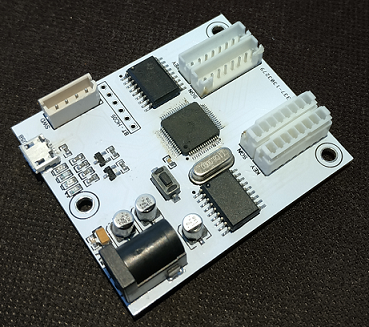
\includegraphics[width=0.5\linewidth]{img/elektronika_moja.png}
    \caption{Zaprojektowany układ elektroniczny do obsługi sztucznej skóry}
    \label{f_elektronika_moja}
\end{figure}

Do poprawnego działania sterownika potrzebny jest mikrokontroler. Wybór padł na opisywany już wcześniej w tej pracy STM32, a~dokładniej STM32F103RB. Mikrokontroler ten jest bardzo prosty, posiada niewielką ilość pamięci Flash i podstawowe peryferia. Pośród posiadanych przez niego peryferiów znajdują się kluczowe dla tego projektu przetworniki analogowo-cyfrowe, które pozwalają na bezpośrednie odczytywanie wartości napięcia na odpowiednim wejściu mikrokontrolera. Przetworniki analogowo-cyfrowe zostały w taki sposób, aby bezpośrednio mierzyć napięcie odkładające się na polu czujnika sztucznej skóry. Schemat podłączenia przetworników analogowych do sztucznej skóry widoczny jest na rysunku \ref{f_elektronika_schemat}. Pozostałe wykorzystywane w tym projekcie peryferia mikrokontrolera nie miały dużego znaczenia przy wyborze modelu, ponieważ znajdują się one w prawie każdym dostępnym na rynku mikrokontrolerze. Mimo wszystko przy wyborze największe znaczenia miała moja wcześniejsza znajomość z tym konkretnym modelem \cite{b_site_F103RB}.

\begin{figure}[!h]
    \centering 
    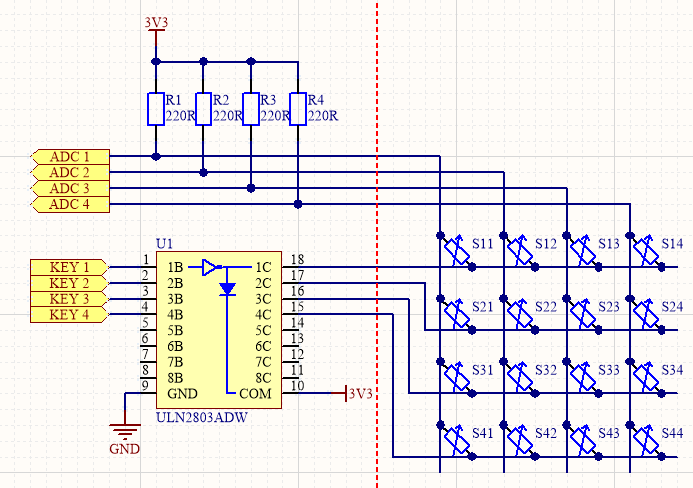
\includegraphics[width=0.95\linewidth]{img/elektronika_schemat.png}
    \caption{Schemat elektroniczny sposobu działania sztucznej skóry}
    \label{f_elektronika_schemat}
\end{figure}

Na schemacie połączeniowym, przedstawionym na rysunku \ref{f_elektronika_schemat}, widoczny jest także układ ULN2803ADW. Układ ten jest drabinką Darlingtonową (drabinką tranzystorów bipolarnych połączonych w~układ Darlingtona) i pełni funkcję klucza zwierającego poziome wiersze czujnika do masy. W~praktyce nie zwiera tych linii do masy tylko do wartości około $0.75 V$, co było mocno widoczne na możliwym do uzyskania zakresie pomiarów, który z~tego powodu był dużo mniejszy \cite{b_site_ULN2803}. Do układu dochodzi sygnał kluczujący, który steruje aktualnie wybranym wierszem, przy czym w danej chwili tylko jeden z nich może być wybrany. W przeciwnym wypadku pomiary będą błędne.

Konstrukcję elektroniczną uzupełniają dość standardowe elementy jak przycisk resetu mikrokontrolera, diody LED sygnalizujące stan pracy urządzenia, stabilizatory ustalające napięcie pracy układu, czy też zabezpieczenia źródła zasilania. Jeśli chodzi o zabezpieczenia, to jako wystarczające zabezpieczenia dla tego projektu uznane zostały: zabezpieczenie przeciwzwarciowe, nadnapięciowe i przed odwróconą polaryzacją źródła zasilania. Zabezpieczenia te zostały zostały dodane w razie potrzeby, ale z racji specyfiki pracy i zasilania przez port USB nie powinny one nigdy zostać w pełni wykorzystane.


% \subsubsection{Oprogramowanie mikrokontrolera}
\subsection{Warstwa programowa}
\label{ss_budowa_prog}

Oprogramowanie jest zwieńczeniem pracy nad sterownikiem. Zespala ono wszystkie spełniane funkcje oraz sprawia, że całość zaczyna spełniać swoje zadanie. Napisany program spełnia wymagania stawiane mu przez pozostałe elementy systemu oraz prawidłowo odczytuje, przetwarza i~interpretuje dane. Zawiera też kilka usprawnień względem kodu przekazanego wraz z prototypem. Program zawiera też w~sobie kilka podstawowych zabezpieczeń. Jednym z~nich jest zabezpieczenie watchdog przed utknięciem w~pętli lub zatrzymaniem działania. 

Główna część programu, zajmująca się przetwarzaniem wyników, pracuje w przerwaniu inicjowanym przez licznik. Część ta jest wywoływana przez program dokładnie z~częstotliwością $10 Hz$. Program w tym momencie wykonuje odczyty napięcia ze~wszystkich zapisanych w~konfiguracji czujników. Aby proces ten przebiegał szybko i~sprawnie przetworniki analogowo-cyfrowe zostały skonfigurowane we współpracy z DMA (direct memory access), który pozwala na przesyłanie danych z~peryferiów do pamięci bez wykorzystania procesora. Zestaw ten znacznie przyspiesza pomiary i~pozwala na~ich wykonywanie w~czasie kiedy procesor przetwarza dane z poprzedniego pomiaru. Po~wykonaniu wszystkich pomiarów dane są obliczane według opisanego dalej algorytmu, a~otrzymany wynik jest wysyłany do komputera.


\subsubsection{Opracowanie algorytmu obliczającego nacisk na wszystkie pola}
\label{sss_budowa_opracowanie_algorytmu}

Algorytm obliczający siłę i kierunek nacisku został napisany tak, aby agregować odczyty ze wszystkich pól czujnika i~przesłać je dalej w prostszej formie. Algorytm zakłada, że~każde pole czujnika jest umiejscowione na robocie i można opisać jego położenie za~pomocą odległości od środka robota i kierunkiem (kątem od środka osi robota). Zależność ta może być przestawiona jako wektory w dwuwymiarowym układzie współrzędnych biegunowych.

Obliczanie końcowego wektora siły odbywa się przez dodawanie do siebie wektorów z kolejnych pól czujnika. Po dodaniu wszystkich wektorów otrzymywany jest wektor wyjściowy siły nacisku i kierunku, który wysyłany jest później do jednostki nadrzędnej. W~ten sposób przesyłana dalej jest tylko kluczowa dla robota część informacji.

Obliczanie kolejnych wektorów siły jest wykonywane za pomocą opisanego algorytmu powtarzanego dla wszystkich pól:
\begin{align}
    F_x & = F_0 * cos(\alpha_0) + F_i * cos(\alpha_i) \\
    F_y & = F_0 * sin(\alpha_0) + F_i * sin(\alpha_i) \\
    F_0 & = \sqrt{F_x^2+F_y^2} \\
    \alpha_0 & = atan2(F_y,F_x)
\end{align}

We wzorze tym $F_i$ jest wartością siły odczytywanej z każdego kolejnego, $i$-tego pola sztucznej skóry. Analogicznie $\alpha_i$ jest wartością kąta kolejnych, $i$-tych pól sztucznej skóry. Zmienna $F_0$ jest skumulowaną wartością siły ze wszystkich kolejnych odczytanych pól sztucznej skóry, aż do $i$-tego pola. Podobnie $\alpha_0$ jest wynikową wartością kąta obliczonej siły $F_0$. Wartości $F_x$ i $F_y$ są chwilowymi przekształceniami siły nacisku oraz jej kąta z układu współrzędnych biegunowych na ich odpowiedniki w układzie kartezjańskim. Otrzymywane są w ten sposób wektory siły nacisku na robota w osiach $x$ i $y$. Przekształcenie wartości siły nacisku na układ kartezjański pozwala kumulować wektory siły odczytywane z kolejnych pól czujnika przez ich sumowanie.

Należy też zauważyć, że siła nacisku $F_i$ w powyższym równaniu obliczana jest bezpośrednio na podstawie odczytów z danego pola czujnika i jest obliczana na podstawie wyznaczonej eksperymentalnie hiperboli aproksymującej czujnik (wyznaczanie hiperboli zostało opisane w rozdziale \ref{ss_badanie_hiperbola}). Siła nacisku $F_i$ jest również na tym etapie dodatkowo dzielona przez odległość od środka robota, aby zmniejszyć wpływ skrajnie zewnętrznych pól czujnika i wzmocnić te bliżej środka robota (lub bardziej strategiczne). Wzmacnianie i~osłabianie wartości siły pochodzącej z czujnika ma na celu priorytetowanie niektórych stref zderzeniowych robota, tak aby te bardziej strategiczne posiadały potencjalnie większą ochronę, przy ewentualnym nacisku na kilka stref jednocześnie.

Podczas późniejszych badań i testów na symulacji zostały wprowadzone modyfikacje do kodu, których nie było w trakcie wcześniejszych badań, a usprawniły pracę nowo zbudowanego prototypu. Modyfikacja była prosta i odcinała niskie, zaszumione pomiary, aby~nie były brane pod uwagę do dalszych obliczeń. Próg odcinania został ustalony na~poziomie $\sim30g$, tak aby nacisk materiału nośnego nie wprowadzał robota w błąd. Błędy wynikające z nieodcinania niskich wartości stały się widoczne, ponieważ wykorzystywana konfiguracja była mocno niesymetryczna i pomiary z przeciwnych stron nie niwelowały się. Poprzez wprowadzenie granicy odcięcia sygnału podczas braku nacisku na sztuczną skórę zwracała ona jako wynik dokładnie $0$.

\subsubsection{Weryfikacja opracowanego algorytmu obliczającego nacisk}
\label{sss_budowa_weryfikacja_algorytmu}

Wyznaczony algorytm poza sprawdzeniem teoretycznym (obliczenia matematyczne) przetestowany został także w praktyce i to praktyczne podeście było najważniejszym testem dla zaproponowanego algorytmu. Praktyczne podejście pozwala wziąć pod uwagę elementy, których nie ma w teoretycznych obliczeniach - szumy i zakłócenia. 

Dla przyspieszenia badań wykorzystany został przekazany prototyp, ale z nowym już układem elektronicznym i oprogramowaniem. Układ sterowania zaprogramowany został tak, aby każde z pól miało tą samą wartość odległości, aby wszystkie pola miały taki sam priorytet. Część pól sensora odpowiedzialna za kąt rozplanowana została na planie zegara, z centrum tarczy w środku. Kąty poszczególnych pól zostały określone przez obliczanie ich położenia względem wcześniej wybranego kierunku 0, poprzez wzrastanie kąta przeciwnie do wskazówek zegara.
Pełna wgrana konfiguracja prototypu przygotowanego do testów została przedstawiona w tabeli \ref{t_badanie0_config}.

\begin{table}[!h]
\centering
\caption{Wgrana konfiguracja czujnika do testów algorytmu obliczającego nacisk}
\begin{tabular}{|l|l|rrrr|}
\hline
\rowcolor[HTML]{FFFFFF} 
 &
   &
  \multicolumn{1}{l|}{\cellcolor[HTML]{FFFFFF}Kolumna 1} &
  \multicolumn{1}{l|}{\cellcolor[HTML]{FFFFFF}Kolumna 2} &
  \multicolumn{1}{l|}{\cellcolor[HTML]{FFFFFF}Kolumna 3} &
  \multicolumn{1}{l|}{\cellcolor[HTML]{FFFFFF}Kolumna 4} \\ \hline
\rowcolor[HTML]{C0C0C0} 
\cellcolor[HTML]{FFFFFF}                         & Kąt       & 135° & 105° & 75°  & 45°  \\ \cline{2-2}
\rowcolor[HTML]{EFEFEF} 
\multirow{-2}{*}{\cellcolor[HTML]{FFFFFF}Rząd 1} & Odległość & 1    & 1    & 1    & 1    \\ \cline{1-2}
\rowcolor[HTML]{C0C0C0} 
\cellcolor[HTML]{FFFFFF}                         & Kąt       & 165° & 135° & 45°  & 15°  \\ \cline{2-2}
\rowcolor[HTML]{EFEFEF} 
\multirow{-2}{*}{\cellcolor[HTML]{FFFFFF}Rząd 2} & Odległość & 1    & 1    & 1    & 1    \\ \cline{1-2}
\rowcolor[HTML]{C0C0C0} 
\cellcolor[HTML]{FFFFFF}                         & Kąt       & 195° & 225° & 315° & 345° \\ \cline{2-2}
\rowcolor[HTML]{EFEFEF} 
\multirow{-2}{*}{\cellcolor[HTML]{FFFFFF}Rząd 3} & Odległość & 1    & 1    & 1    & 1    \\ \cline{1-2}
\rowcolor[HTML]{C0C0C0} 
\cellcolor[HTML]{FFFFFF}                         & Kąt       & 225° & 255° & 285° & 315° \\ \cline{2-2}
\rowcolor[HTML]{EFEFEF} 
\multirow{-2}{*}{\cellcolor[HTML]{FFFFFF}Rząd 4} & Odległość & 1    & 1    & 1    & 1    \\ \cline{1-2}
\hline
\end{tabular}
\label{t_badanie0_config}
\end{table}

Część praktyczna badań została przeprowadzona poprzez ustawianie obiektu o znanej masie na prototypie i~odczycie pomiarów zwracanych przez sterownik i~wypisywanych w~oknie konsoli programu PuTTY \cite{b_site_putty}. Przedmiotem użytym do obciążania czujnika była puszka o masie $454 g$. Ważną uwagą dotyczącą użytej puszki jest jej kształt, a dokładniej to, że~posiadała ona okrągły rant o średnicy $72mm$ w dolnej części puszki, który jako pierwszy dotykał powierzchni gumy i~rozprowadzał nacisk na większą powierzchnię. Obciążenie było przykładane kolejno w losowych miejscach i~odczytywane były wartości wyświetlane w konsoli. Wykonane testy zostały przedstawione na rysunku \ref{f_badanie0_pomiary}, a odpowiadające poszczególnym przykładom wyniki pomiarów w~tabeli \ref{t_badanie0_wyniki}.

\begin{figure} [!h]
  \begin{subfigure}[b]{0.5\linewidth}
    \centering
    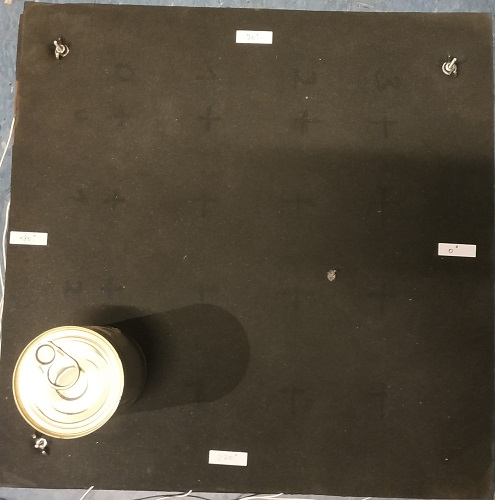
\includegraphics[width=0.75\linewidth]{img/badanie0_1.jpg} 
    \caption{Test 1} 
    % \vspace{4ex}
  \end{subfigure}%% 
  \begin{subfigure}[b]{0.5\linewidth}
    \centering
    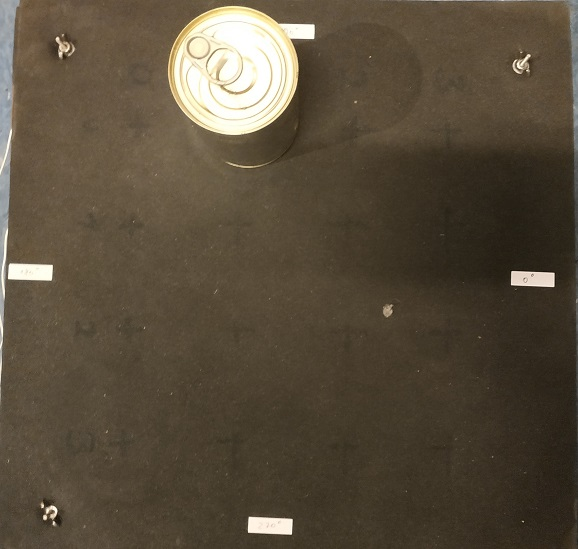
\includegraphics[width=0.75\linewidth]{img/badanie0_2.jpg}
    \caption{Test 2} 
    % \vspace{4ex}
  \end{subfigure} 
  
  \begin{subfigure}[b]{0.5\linewidth}
    \centering
    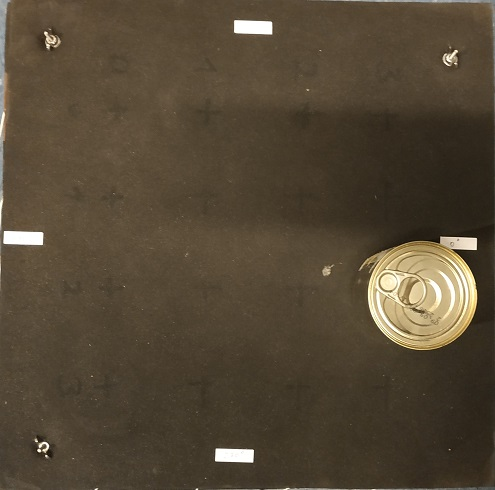
\includegraphics[width=0.75\linewidth]{img/badanie0_3.jpg} 
    \caption{Test 3}
  \end{subfigure}%%
  \begin{subfigure}[b]{0.5\linewidth}
    \centering
    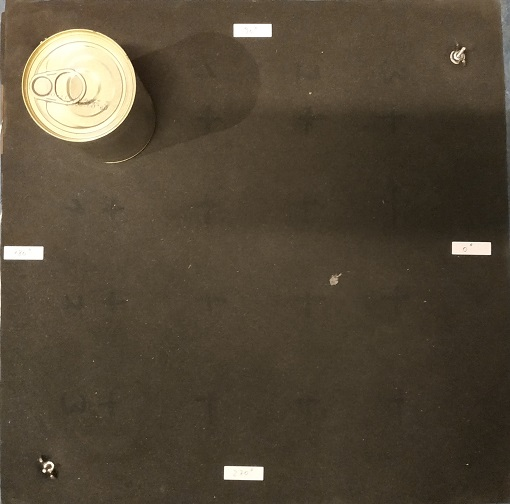
\includegraphics[width=0.75\linewidth]{img/badanie0_4.jpg}
    \caption{Test 4}
  \end{subfigure} 
  
  \begin{subfigure}[b]{0.5\linewidth}
    \centering
    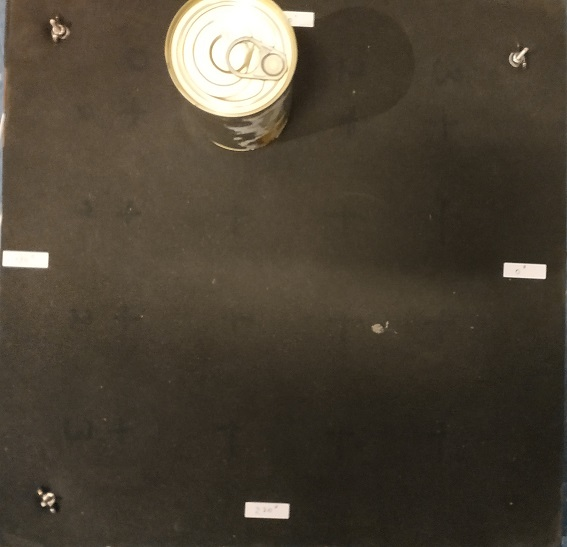
\includegraphics[width=0.75\linewidth]{img/badanie0_5.jpg}
    \caption{Test 5}
  \end{subfigure}%%
  \begin{subfigure}[b]{0.5\linewidth}
    \centering
    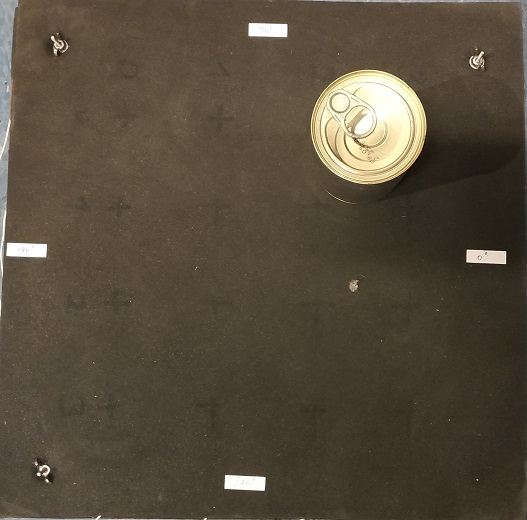
\includegraphics[width=0.75\linewidth]{img/badanie0_6.jpg}
    \caption{Test 6}
  \end{subfigure} 
  \centering
  \caption{Testy działania zaprogramowanego czujnika weryfikujące algorytm obliczający nacisk}
  \label{f_badanie0_pomiary} 
\end{figure}

\begin{table}[!h]
\centering
\caption{Wyniki testów algorytmu obliczającego nacisk}
\begin{tabular}{|l|r|r|}
\hline
Test   & \multicolumn{1}{l|}{Kąt} & \multicolumn{1}{l|}{Siła} \\ \hline
Brak obciążenia   & 45-50°                   & 40                        \\ \hline
Test 1 & 221°                     & 300                       \\ \hline
Test 2 & 100°                     & 500                       \\ \hline
Test 3 & 347°                     & 730                       \\ \hline
Test 4 & 134°                     & 670                       \\ \hline
Test 5 & 104°                     & 420                       \\ \hline
Test 6 & 45°                      & 700                       \\ \hline
\end{tabular}
\label{t_badanie0_wyniki}
\end{table}

Pierwszy pomiar zawiera wynik zwracany przez sterownik w momencie, kiedy prototyp nie był obciążony żadnym przedmiotem. Jak możemy zauważyć występuje tam szum, którego wartości cały czas nieznacznie się wahały. Otrzymywany szum nie osiągał dużych wartości i mógł zostać pominięty.

Kolejne pomiary wykonane z obciążeniem okazały się bardzo dobrze odwzorowywać miejsce przykładanej siły, nawet z obciążeniem znajdującym się pomiędzy polami czujnika. Z kolei w przypadku określania wartości przykładanej siły nacisku wyniki wydają się być niejednoznaczne. Otrzymywana wartość siły nacisku oscylowała podczas testów (również niezawartych w pracy) w granicach $300 - 750 g$ podczas, gdy prawdziwa waga obciążenia wynosiła $454 g$. Otrzymane w ten sposób wyniki posiadają bardzo złą dokładność względną pomiaru wynoszącą $-34\%/+65\%$. Mimo tak dużych rozbieżności pokazuje to pewną zależność, a same wyniki oscylują wokół faktycznej wagi i bardzo dobrze oddają kąt przyłożonej siły.

W celu znalezienia przyczyny tych rozbieżności wykonane zostało kilka niestandardowych pomiarów, gdzie to samo obciążenie ($454g$) było ustawione na krawędzi puszki czyniąc obszar nacisku dużo bardziej punktowym. W kolejnych testach zmieniany był punkt na prototypie, na którym spoczywało obciążenie. W ten sposób pomiary zostały wykonane zarówno idealnie na polu pomiarowym, jak i pomiędzy polami. Jak się okazało punkt przyłożenia obciążenia miał kluczowe znaczenie na otrzymywany wynik. Przy ułożeniu puszki na brzegu, bezpośrednio nad polem otrzymywane wyniki pomiarów były rzędu $\sim1100g$, a pomiędzy polami spadały one nawet do wartości $\sim200g$. Z otrzymanych danych jasno wynika, że miejsce przyłożenia nacisku ma duże znaczenie na odczytany pomiar i z tego powodu wykonane wcześniej pomiary posiadają tak duży rozrzut wartości zmierzonej masy. Może to świadczyć o tym, że materiał nośny niezbyt dobrze radzi sobie z rozkładaniem przyłożonej siły na boki, zamiast tego przenosi ją w~głąb, jednocześnie się uginając. Dodatkowo folia Velostat z racji, iż jest czujnikiem rezystancyjnym pokazuje dużo wyższe wyniki pomiarów w przypadku przyłożenia siły w jednym punkcie, niż~w~przypadku przyłożenia tej samej siły na większej powierzchni, nawet kiedy rozkłada się ona w całości na polu czujnika. Dodatkowe czynniki wpływające na wynik pomiaru zostały wykryte i~szczegółowo opisane w dalszych testach opisanych w dalszej części pracy.


% \subsubsection{Komunikacja przez USB}
\subsection{Warstwa komunikacyjna}
\label{ss_budowa_kom}

Komunikacja sterownika z komputerem nadrzędnym jest częścią, która stanowi o~użyteczności modułu sztucznej skóry. Jej rola polega na ciągłym i stabilnym wysyłaniu odbieranych informacji o otoczeniu do komputera sterującego całym robotem. Bez tej funkcji nawet poprawnie działająca sztuczna skóra nie ma żadnej wartości w systemie robota, ponieważ sam robot nie żadnych informacji o tym, że czujnik skóry cokolwiek wykrył.

Zastosowany w ramach pracy sposób komunikacji powinien być opisany powszechnie znanymi i rozpowszechnionymi standardami. Takie podejście pozwala na wybranie gotowych rozwiązań i na nietworzenie własnych, nie zawsze sprawdzonych rozwiązań. W~tym celu wybrane zostało jedno z najpopularniejszych obecnie rozwiązań - USB w standardzie 2.0. Gniazda w tym standardzie znajdują się obecnie w większości komputerów, również w urządzeniu, do którego sterownik będzie bezpośrednio dołączany. Standard ten wprowadzony już w 2000 roku oferuje prędkość przesyłu danych do 480Mbs, co jest w~pełni wystarczające dla obsługi sztucznej skóry. Wraz z samą komunikacją standard USB zapewnia zasilanie 5V dostarczane przez komputer. Pozwoliło to zasilić sterownik tym samym przewodem, po którym poprowadzona była komunikacja. Standard specyfikuje także przewody i gniazda, które można bez problemu nabyć na rynku \cite{b_manual_USB}.

Wykorzystanie do komunikacji standardu USB zmusiło mnie do wykonania projektu, który spełnia jego standardy. Nie zostały wybrane jednak mikrokontrolery STM z przeznaczonym do tego peryferium. Powodem takiej decyzji był chwilowy brak dostępności mikrokontrolerów o szukanych parametrach w tak małej (64 piny) obudowie układu scalonego. Problematyczna okazywała się także kwestia konieczności doinstalowania odpowiednich sterowników na komputerze do obsługi tak wykonanego układu. Dlatego ostatecznie do~komunikacji USB został wykorzystany dedykowany do tego układ CP2102 od Silicon Labs, który został zintegrowany na płytce drukowanej. Układ ten jest zgodny ze standardem USB 2.0 i pozwala na komunikację z prędkością do 12Mbs, co dla opracowywanego zastosowania jest wystarczające. Układ CP2102 jest konwerterem USB-UART co oznacza, że do poprawnej komunikacji mikrokontroler musi używać standardu UART. Standard UART jest dużo mniej skomplikowany niż wspomniany wcześniej USB, prostszy w obsłudze i~programowaniu. Konfiguracja wykorzystanego portu UART prezentowała się następująco: szybkość transmisji - 115200, liczba bitów - 8, bit parzystości - brak, bit stopu - 1. Układ CP2102 do poprawnej pracy wymaga również zainstalowania odpowiednich sterowników dostępnych na stronie producenta. Sterowniki te są również automatycznie instalowane wraz z systemem Linux Ubuntu \cite{b_site_CP2102}, na którym działał komputer nadrzędny.
% mikrokontroler

Aktualny projekt części elektronicznej zakłada również możliwość rozbudowy o dodatkowe sposoby komunikacji z komputerem nadrzędnym. Posiada wyprowadzone dodatkowe złącze, które może posłużyć właśnie do tego celu. Złącze to jest przystosowane bezpośrednio do~podłączenia tam popularnego modułu Bluetooth HC-05 \cite{b_site_HC-05_sklep}. Umożliwia to w przyszłości wykorzystanie urządzenia w systemach bezprzewodowych, czy też rozwiązaniach IOT.

Po ustaleniu wykorzystywanych fizycznie elementów ustalony został także standard przesyłanych informacji. W tym przypadku nie zostało wykorzystane żadne z istniejących i ustandaryzowanych rozwiązań. Standardy dostępne na rynku wymagają większych mocy obliczeniowych i czasowych do poprawnej pracy, w szczególności do obsługi błędów.
Dlatego zaimplementowane zostało dużo prostsze rozwiązanie, które w przeciwieństwie do standardów nie posiada tak dobrych zabezpieczeń. Wykorzystanie własnej implementacji zapewnia natomiast prostotę rozwiązania i niewielki nakład energii potrzebny do~przesłania danych.

Ramki przesyłające informacje są różne, w zależności od kierunku przesyłu danych. Ramka przesyłana do sterownika posiada lepszy opis i dokładny format ramek, aby nie zmienić konfiguracji sterownika przypadkowo. Ogólny wygląd przesyłanej ramki został przedstawiony w tabeli \ref{t_ramka_ogolna}, a dokładna zawartość przesyłanych danych w zależności od~funkcji w tabeli \ref{t_ramka_funkcja}. Ramki zaprojektowane w ten sposób zapewniają kilka podstawowych zabezpieczeń. Posiadane zabezpieczenia obejmują: pasywne zabezpieczenie przeciw przerwanym wiadomościom, zbyt długi czas przesyłu danych i możliwym zakłóceniom połączenia.

\begin{table}[!h]
\centering
\caption{Ramka danych przesyłanych przez USB do sterownika}
\begin{tabular}{|l|l|l|l|l|}
\hline
            & \multicolumn{1}{|c|}{Prefiks} & \multicolumn{1}{|c|}{Funkcja}                 & \multicolumn{1}{|c|}{Przesyłane dane}    & \multicolumn{1}{|c|}{Sufiks} \\ \hline
Liczba bajtów & 1      & 1                       & 7                  & 1      \\ \hline
Zawartość   & 0x02   & Typ przesyłanych danych & Dane do przesłania & 0x03   \\ \hline
\end{tabular}
\label{t_ramka_ogolna}
\end{table}

\begin{table}[!h]
\small
\centering
\caption{Tabela funkcji dostępnych w ramkach przesyłanych do sterownika}
\begin{tabular}{|l|l|c|l|l|l|l|l|l|}
\hline
\multicolumn{1}{|c|}{Funkcja} &
  \multicolumn{1}{c|}{\begin{tabular}[c]{@{}c@{}}Kod \\ funkcji\end{tabular}} &
  \multicolumn{7}{c|}{Dane} \\ \hline
\begin{tabular}[c]{@{}l@{}}Wyczyszczenie \\ pamięci\end{tabular} &
  0x01 &
  \multicolumn{7}{c|}{Bez znaczenia} \\ \hline
\begin{tabular}[c]{@{}l@{}}Potwierdzenie \\ wysłanych danych\end{tabular} &
  0x02 &
  \multicolumn{7}{c|}{Bez znaczenia} \\ \hline
\begin{tabular}[c]{@{}l@{}}Programowanie \\ pola czujnika \\ dotykowego\end{tabular} &
  0x10 &
  \multicolumn{1}{l|}{\begin{tabular}[c]{@{}l@{}}Pozostała\\ liczba pól\\ (1 bajt)\end{tabular}} &
  \begin{tabular}[c]{@{}l@{}}Klucz\\ (1 bajt)\end{tabular} &
  \begin{tabular}[c]{@{}l@{}}Kanał\\ (1 bajt)\end{tabular} &
  \multicolumn{2}{l|}{\begin{tabular}[c]{@{}l@{}}Kąt \\ (2 bajty)\end{tabular}} &
  \multicolumn{2}{l|}{\begin{tabular}[c]{@{}l@{}}Odległość \\ (2 bajty)\end{tabular}} \\ \hline
\end{tabular}
\label{t_ramka_funkcja}
\end{table}

Dane przesyłane do sterownika muszą zaczynać się od prefiksu, a kończyć sufiksem. Są one konieczne, aby sterownik mógł poprawnie otrzymać i zinterpretować przesyłane dane. Wewnątrz znajdują się przesyłane funkcje, których jest niewiele, ale wystarczają do~poprawnego działania sterownika. Funkcja czyszczenia pamięci jest konieczna, aby~poprawnie zaprogramować sterownik - wykonuje ona resetowanie pamięci Flash mikrokontrolera. Potwierdzenie wysłanych danych jest funkcją wysyłaną jako ostatnia, jako potwierdzenie zakończenia transmisji danych. Wysłanie tej funkcji pozwala na przejście programu mikrokontrolera do normalnej pętli pracy i wysyłanie pomiarów z czujnika do komputera. Niewysłanie tej funkcji wymaga zrestartowania mikrokontrolera, w~celu umożliwienia mu wysyłania danych do komputera.

Ostatnią i najważniejszą funkcją jest wysyłanie sterownikowi konfiguracji czujnika. Kod funkcji oznacza typ pola (w tym momencie jest jeden, ale w przyszłości można zaimplementować więcej). Po nim wysyłana jest liczba pól danego typu, które jeszcze zostaną przesłane. Ta informacja zapewnia spójność wysyłanych danych i zapobiega nieoczekiwanemu przerwaniu transmisji. Kolejno przesyłane są współrzędne pola (klucz i~kanał), jego wartość kąta wychylenia w~osi~$z$~robota oraz odległość czujnika od~środka robota.

Ramki przesyłane ze sterownika do komputera miały całkowicie inny kształt. Były one przeznaczone do bezpośredniego wyświetlania wysyłanych wartości na konsoli komunikacyjnej (w moim przypadku w programie PuTTY). Przesyłane liczby są wysyłane jako znaki zakodowane kodem ASCII, co wynika z konieczności ich bezpośredniego wyświetlania. Wysyłane przez sterownik ramki są przedstawione w tabeli \ref{t_ramka_przychodzi}. Wysyłanie wiadomości w~ten sposób wymagało dodatkowych przekształceń po obu komunikujących się stronach. Zmniejszyło to też wymiar przesyłanych danych do wartości 4-liczbowych. Takie podejście, mimo większej ilości zużywanych zasobów po obu stronach, pozwala na dużo szybszą i wygodniejszą współpracę ze sterownikiem, a także możliwość wykrywania błędów na~konsoli dowolnego komputera.

\begin{table}[!h]
\footnotesize
\centering
\caption{Ramka danych wysyłanych przez USB przez sterownik}
\begin{tabular}{|l|l|l|l|l|}
\hline
Wartość obliczonego kąta &
  , &
  Wartość obliczonej siły &
  ; &
  Przejście do następnej linii \\ \hline
\multicolumn{1}{|c|}{\begin{tabular}[c]{@{}c@{}}4 bajty - cyfry \\ kodowane ASCII\end{tabular}} &
  \multicolumn{1}{c|}{0x2C} &
  \multicolumn{1}{c|}{\begin{tabular}[c]{@{}c@{}}4 bajty - cyfry \\ kodowane ASCII\end{tabular}} &
  \multicolumn{1}{c|}{0x3B} &
  \multicolumn{1}{c|}{\begin{tabular}[c]{@{}c@{}}0x0D0A - znak powrotu\\ karetki i nowej linii\end{tabular}} \\ \hline
\end{tabular}
\label{t_ramka_przychodzi}
\end{table}

Ramka przesyłana przez sterownik do komputera, jak widać w tabeli \ref{t_ramka_przychodzi}, jest dużo prostsza i~ma tylko jedną konfigurację wypełnianą odpowiednimi danymi. Pierwsza część zawiera wartość obliczonego przez algorytm kąta siły, później dla czytelności i~oddzielenia danych wysyłany jest przecinek. Kolejną wysyłaną informacją jest wartość samej siły nacisku. Na koniec wysyłane są średnik oraz sekwencja znaków przenosząca karetkę (wskaźnik pisania na konsoli) na początek następnej linii konsoli.

\newpage
\section{Statyczne badanie właściwości sztucznej skóry}
\label{s_badanie}

Badania właściwości statycznych obejmowały duży zakres prac wykonanych podczas pisania tego dokumentu. Były one podstawą do pogłębiania wiedzy z zakresu działania i zachowania sztucznej skóry oraz posłużyły do budowy prototypu sztucznej skóry umieszczonej później na robocie. 

Badania wykonane przeze mnie były kontynuacją badań prowadzonych przez inż. Macieja Bogusza opisanych w cytowanej przeze mnie pracy. W swoich pracach badał on wiele różnych typów gumy pod kątem przewodności elektrycznej, trwałej odkształcalności oraz pochłanialności energii. Jego badania miały na celu wybór najlepszego materiału nośnego i absorbującego uderzenia, który mógłby posłużyć do budowy sztucznej skóry. Wykonał on także prototyp do~dalszych testów o rozmiarze $4x4$ pola ($25 cm^2$ każde) i~wielkości $40x40 cm$ dwóch fragmentów mikrogumy o grubości $10mm$, każda jako warstwa nośna. Prototyp ten był niego testowany w specjalnie napisanej aplikacji pokazującej napięcie odczytywane na poszczególnych polach czujnika 
\cite{b_report_otrzymane}.

Prowadzone w ramach pracy badania skupiały się na wykonaniu pełnej charakterystyki pojedynczego pola czujnika i ustaleniu równania opisującego zależność pomiędzy przykładanym naciskiem, a odczytywanym napięciem na badanym polu. To badanie jest podstawowym badaniem potrzebnym do obliczeń siły nacisku i umożliwia późniejsze zastosowanie sztucznej skóry w pełni kontrolowany sposób.

Dalsza część badań opierała się na dobraniu zewnętrznych warstw nośnych czujnika, ponieważ wewnętrzne (taśma miedziana i folia Velostat) okazują się działać bardzo dobrze i nie było w nich znacznego pola na poprawę jakości sztucznej skóry. Badania warstw nośnych polegały na doborze odpowiedniej grubości tego samego rodzaju gumy NBR190. Polegały one na pomiarze właściwości gum, pochłanialności energii i rozkładaniu energii przez gumy. Aby poprawnie symulować zachodzące procesy i zapewnić wiarygodne pomiary, badania były przeprowadzane na specjalnie do tego przygotowanych wersjach czujnika. Przygotowane czujniki posiadały tylko jedno pole i pozwalały na~dowolną zamianę górnej i dolnej warstwy nośnej, tak aby przebadać wszystkie możliwe kombinacje budowy czujnika z posiadanych grubości gum. Do badań przygotowane zostały gumy o~grubościach: $5mm$, $10mm$, $15mm$ i $20mm$, z których wycięto pola w~kształcie kwadratu o wymiarach $100x100 mm$. Do każdego z tak przygotowanych pól przyklejono taśmę miedzianą o szerokości $50 mm$. Pomiędzy taśmą miedzianą z dolnej warstwy czujnika i~górnej warstwy czujnika umieszczono docięty na wymiar fragment folii Velostat. Tak~przygotowany czujnik był wykorzystywany w dalszych badaniach.

\subsection{Pomiar zależności masa -- odczyt pojedynczego pola}
\label{ss_badanie_hiperbola}

Pomiar zależności odczytów czujnika w zależności od przyłożonej masy jest pierwszym wykonywanym badaniem, ponieważ jest on kluczowy do wszystkich obliczeń. Bez~znajomości tej zależności surowa wartość odczytana z czujnika nie niesie ze sobą żadnej informacji, jest tylko liczbą. Istotą wyprowadzenia tej zależności jest możliwość wstecznego obliczenia przyłożonego nacisku na podstawie zwracanych danych. Należy także sprawdzić, czy poza naciskiem, wykonane pomiary zależą również od innych zmiennych oraz jaka jest dynamika pracy czujnika.

Do testów charakterystyki pojedynczego pola sztucznej skóry została wykorzystana mniejsza jej wersja używająca tylko jednego pola, aby mieć pewność, że nacisk nie rozkłada się na sąsiadujące elementy. Dodatkowo, czujnik został zbudowany z posiadanych laminatów, które zostały zastosowane jako warstwa nośna zamiast sprężystej gumy. Ewentualne używanie gumy jako materiału nośnego mogłoby zakłócić pomiary przez rozprowadzanie przykładanej siły na boki. Do budowy wnętrza czujnika została wykorzystana taśma miedziana o szerokości $50 mm$ i docięta na odpowiednią wielkość folia Velostat. W efekcie pole efektywne zbudowanego czujnika wynosiło $25 cm^2$. Wykonany czujnik pomiarowy został przedstawiony na rysunku \ref{f_badanie_1_czujnik}.

\begin{figure}[!h]
\centering
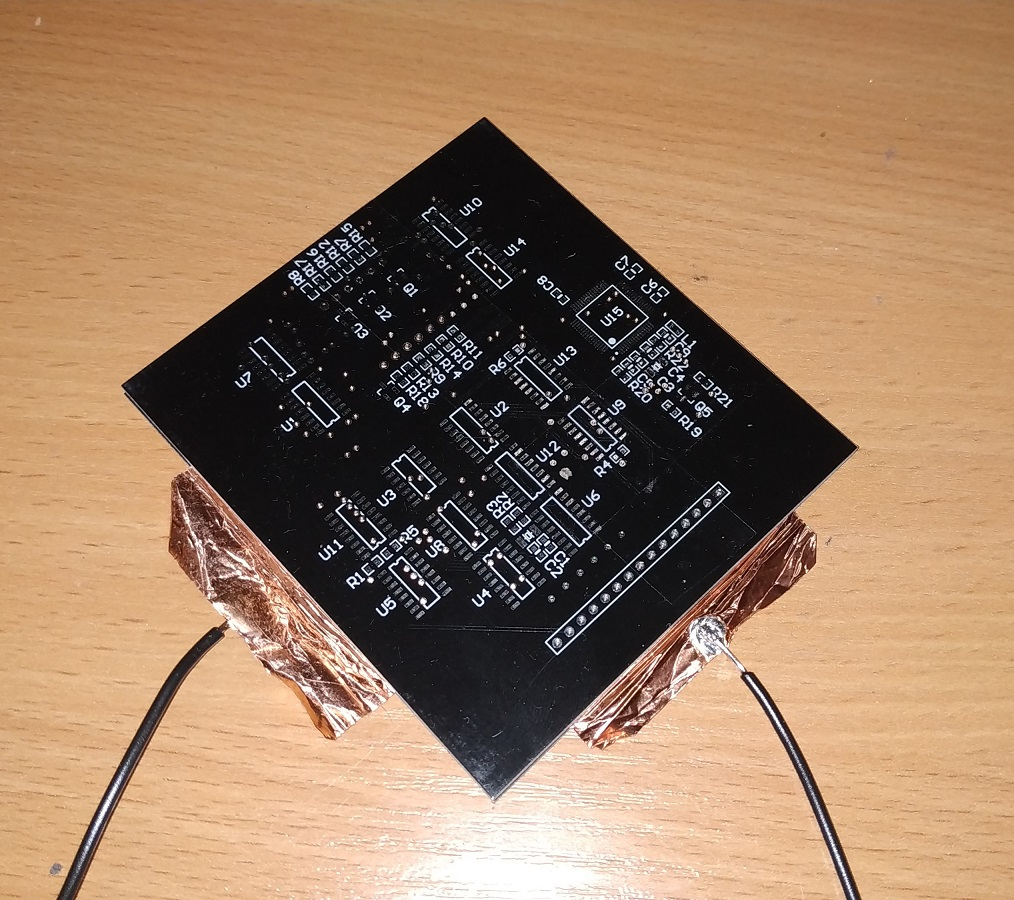
\includegraphics[width=0.5\linewidth]{img/badanie_1_czujnik.jpg}
\caption{Czujnik wykorzystywany do badania charakterystyki folii Velostat}
\label{f_badanie_1_czujnik}
\end{figure}

Wykorzystując zbudowane pole czujnika wyznaczona została charakterystyka jego pracy. Badany był poziom otrzymywanego surowego sygnału w zależności od przykładanego nacisku. Nacisk był wywierany poprzez obciążanie czujnika znaną masą, a surowe pomiary odczytywane w konsoli programu PuTTY.

Pomiary czujnika były zwracane w obszarze $0-3,3V$ co przekłada się na odczyty mikrokontrolera w~zakresie $0-4096$. Taki zakres wynika z wykorzystania wbudowanego w~mikrokontroler STM32F103RB 12-bitowego przetwornika ADC \cite{b_site_F103RB}. Analizując schemat działania czujnika, widoczny na rysunku \ref{f_elektronika_schemat}, możemy zauważyć, że przy braku nacisku (maksymalna rezystancja folii Velostat) otrzymywane są wyniki bliskie maksymalnych możliwych wartości pomiaru ($\sim4000$). Wraz ze zwiększaniem przykładanej siły wartość pomiaru zmniejsza się aż do wartości $\sim1000$. Najniższe uzyskane wartości pomiarów w~okolicy $\sim1000$, a nie $\sim0$ wynikają z użytego układu drabinki Darlingtonowej ULN2803, a~dokładniej z~jej spadku napięcia $V_{CE(sat)}$ wynoszącego w~badanej konfiguracji około $0,75 V$ \cite{b_site_ULN2803}. Pełne wyniki wykonanych pomiarów podczas badań znajdują się w tabeli \ref{t_badanie_1_pomiary}.

\begin{table}[!h]
\centering
\caption{Wykonane pomiary pojedynczego pola czujnika}
\begin{tabular}{|r|r|r|r|r|r|l|}
\hline
\multicolumn{1}{|l|}{Obciążenie {[}g{]}} &
  \multicolumn{1}{l|}{Pomiar 1} &
  \multicolumn{1}{l|}{Pomiar 2} &
  \multicolumn{1}{l|}{Pomiar 3} &
  \multicolumn{1}{l|}{Pomiar 4} &
  \multicolumn{1}{l|}{Pomiar 5} &
  Pomiar 6 \\ \hline
1     & 3930 & 3900 & 3900 & 3870 & 3800 & \multicolumn{1}{r|}{3800} \\ \hline
23    &      &      & 3830 & 3820 &      &                           \\ \hline
51    &      &      & 3800 & 3770 &      &                           \\ \hline
66    &      &      & 3740 & 3720 &      &                           \\ \hline
129   &      &      & 3610 & 3570 &      &                           \\ \hline
324   &      &      & 3300 & 3120 &      &                           \\ \hline
461   &      &      & 3000 & 2850 &      &                           \\ \hline
519   & 3000 & 2900 & 2800 & 2500 & 2600 & \multicolumn{1}{r|}{2500} \\ \hline
1037  & 2400 & 2150 & 2210 & 2030 & 2000 & \multicolumn{1}{r|}{1900} \\ \hline
1555  & 1910 & 1840 & 1670 & 1580 & 1530 & \multicolumn{1}{r|}{1540} \\ \hline
2073  & 1670 & 1610 & 1470 & 1380 & 1340 & \multicolumn{1}{r|}{1380} \\ \hline
2591  & 1560 & 1480 & 1300 & 1265 & 1180 & \multicolumn{1}{r|}{1210} \\ \hline
3109  & 1390 & 1340 & 1220 & 1200 & 1130 & \multicolumn{1}{r|}{1130} \\ \hline
3642  & 1290 & 1270 & 1140 & 1111 &      &                           \\ \hline
4175  & 1220 & 1240 & 1100 & 1090 &      &                           \\ \hline
4708  & 1170 &      &      &      &      &                           \\ \hline
5248  & 1140 &      &      &      &      &                           \\ \hline
78000 & 890  &      &      &      &      &                           \\ \hline
\end{tabular}
\label{t_badanie_1_pomiary}
\end{table}

Wyznaczanie charakterystyki polegało na kolejnym obciążaniu czujnika przedmiotami o znanej masie. Czujnik miał bardzo niezadowalającą dynamikę i~ciężko było wyznaczyć jednoznaczną charakterystykę czujnika. Dynamika czujnika objawiała się głównie na~gwałtownym osiągnięciu wartości w okolicy wartości końcowej i późniejszym powolnym dochodzeniu do tej wartości. Osiąganie wartości końcowej czasami zajmowało nawet kilka minut. Ze względu na wykorzystanie czujnika w dość dynamicznym środowisku, które musi szybko reagować na bodźce, nie jest to pożądana charakterystyka. Na~szczęście, czujnik ten też natychmiastowo (w kontekście częstotliwości wykonywanych pomiarów) osiąga wartość w okolicach docelowej. Można ten fakt wykorzystać i~ustalić charakterystykę czujnika w pierwszej fazie po otrzymaniu bodźca.

Układ sprawiał też dziwne wrażenie, jakby z upływam czasu zmieniał swoje odczyty, co jest również widoczne w tabeli \ref{t_badanie_1_pomiary}. Pomiary 1, 2, 3 i 4 wykonane zostały jednego dnia. Pomiary 1 i 2 były prowadzone równolegle - naprzemiennie prowadzono pomiary wartości dla danego obciążenia z chwilowym odpuszczaniem, aby rozluźnić naprężenia czujnika pomiędzy pomiarami. Później, tego samego dnia, wykonane zostały pomiary 3 i 4, mające na celu sprawdzenie szybkości reakcji i wartości końcowej przy danym obciążeniu. Pomiar 3 był wykonywany od razu w chwili położenia obciążenia, pomiar 4 został zmierzony na tym samym przedmiocie bez zmian obciążenia w momencie ustabilizowania się odczytów. Pomiary 5 i 6 zostały wykonane kilka dni później, jako pomiary uzupełniające, mające pokazać poprawność i stałość poprzednich pomiarów. 

Nie wszystkie z wykonanych pomiarów zostały wykonane na pełnym zakresie testowym. Brak pomiarów wartości dla niskich obciążeń spowodowany był początkowym brakiem przykładania większej uwagi dla nacisku w tym zakresie, ponieważ nie spodziewano się wywierania tak lekkiego nacisku na powierzchnię robota. 
Pomiar obciążeniem $78000 g$ został wykonany poprzez stanięcie człowieka na czujniku i miał za zadanie ustalić pomiar czujnika przy teoretycznie nieskończonym obciążeniu. Obciążenie $1 g$ dostało umownie przypisane dla braku dodatkowego obciążenia.

Za rozbieżności podczas wykonywania pomiarów odpowiedzialne może być kilka czynników, w tym zmęczenie materiału folii, wpływ temperatury (której nie mierzono dokonując pomiar) i niestała charakterystyka drabinki Darlingtonowej (która też może zmieniać się w zależności od temperatury \cite{b_site_ULN2803}).

% \begin{figure} [!h]
%   \begin{subfigure}[b]{0.5\linewidth}
%     \centering
%     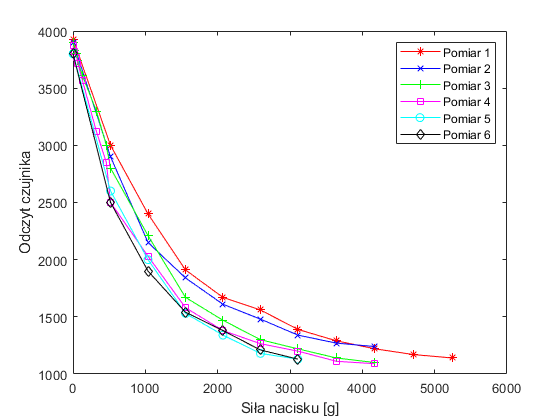
\includegraphics[width=1\linewidth]{img/badanie_1_pomiar.png} 
%     \caption{Pomiary w skali standardowej} 
%   \end{subfigure}%% 
%   \begin{subfigure}[b]{0.5\linewidth}
%     \centering
%     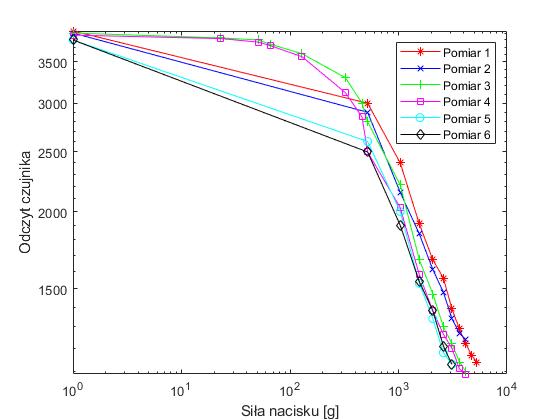
\includegraphics[width=1\linewidth]{img/badanie_1_logarytm.png}
%     \caption{Pomiary w skali logarytmicznej}
%   \end{subfigure} 
%   \centering
%   \caption{Wykonane pomiary pojedynczego pola}
%   \label{f_badanie_1_pomiar} 
% \end{figure}

Pełne wykresy zebranych danych przedstawiono na wykresie \ref{f_badanie_1_standard}, zostały one również przedstawione w skali logarytmicznej na wykresie \ref{f_badanie_1_logarytm}. Wykres z logarytmiczną skalą został wykonany, ponieważ pierwsze spojrzenie na otrzymane pomiary sugerowało charakterystykę logarytmiczną czujnika. Założenie to po przeanalizowaniu wykresu w~skali logarytmicznej okazało się nieprawdziwe.

\begin{figure}[!h]
    \centering 
    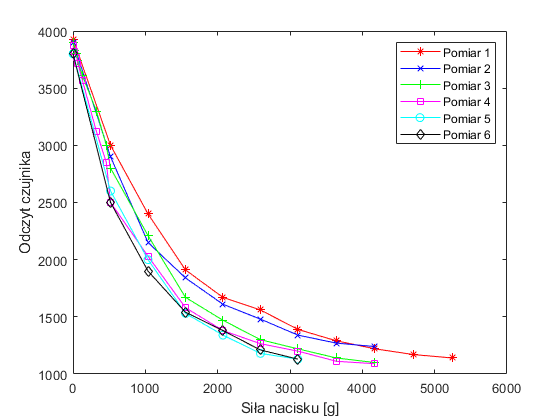
\includegraphics[width=0.85\linewidth]{img/badanie_1_pomiar.png}
    \caption{Wykonane pomiary pojedynczego pola -- skala liniowa}
    \label{f_badanie_1_standard}
\end{figure}

\begin{figure}[!h]
    \centering 
    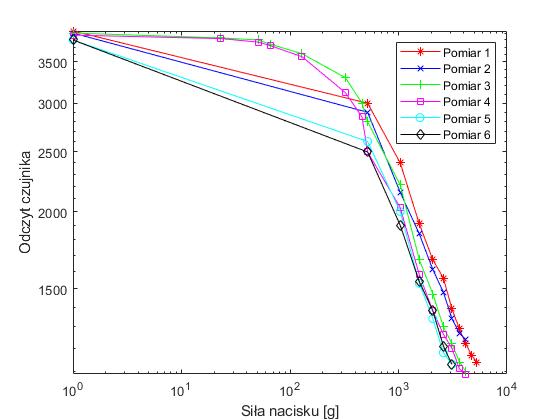
\includegraphics[width=0.85\linewidth]{img/badanie_1_logarytm.png}
    \caption{Wykonane pomiary pojedynczego pola -- skala logarytmiczna}
    \label{f_badanie_1_logarytm}
\end{figure}

Jak można zauważyć, wykonane odczyty układają się w dodatnią część wykresu hiperboli i ten kształt przyjęto w procesie aproksymacji. Standardowe równanie hiperboli ma postać:
\begin{equation}
    f(x) = y + \frac{a}{(x-x_0)}
\end{equation}
gdzie parametry $y$, $a$ i $x_0$ muszą zostać dobrane indywidualnie do naszego przypadku. Parametr $y$ odpowiada za przesunięcie wykresu hiperboli w osi pionowej, $x_0$ za przesunięcie w osi poziomej, natomiast $a$ odpowiada za sam kształt hiperboli.

W celu przyspieszenia wyznaczenia parametrów hiperboli użyty został program Matlab i jego funkcja wbudowana \textit{fminunc}. Funkcja ta jest w stanie znaleźć minimum zadanej funkcji wielu zmiennych używając wybranego algorytmu (Quasi-Newtonowski lub regionu zaufania). Algorytm optymalizacji przyjmuje jako parametr funkcję do optymalizacji (w~analizowanym przypadku - hiperbola), punkt początkowy poszukiwania rozwiązania oraz parametry wpływające na wewnętrzne działanie algorytmu m.in. algorytm działania czy ilość wypisywanych informacji w trakcie obliczeń \cite{b_site_Matlab_fminunc}.

Ważną sprawą podczas używania tego sposobu minimalizacji jest zwracanie przez algorytm minimum lokalnego, co oznacza, że zwrócone rozwiązanie nie musi być najlepsze ze wszystkich istniejących \cite{b_site_Matlab_fminunc}. Dlatego, aby zwiększyć prawdopodobieństwo znalezienia najlepszego rozwiązania, algorytm został uruchomiony wielokrotnie z różnymi, losowymi punktami początkowymi. Jako najlepsze rozwiązanie wybrane zostało to, które zwróciło najmniejszy błąd aproksymacji. Błąd aproksymacji, tak samo jak parametr minimalizacji, został określony jako norma Euklidesowa wszystkich punktów. Równanie normy Euklidesowej opisane jest wzorem:
\begin{equation}
    e = \sqrt{\sum_{i=1}^{n} (f(x_i) - y_i)^2}
\end{equation}
gdzie $e$ jest obliczonym błędem aproksymacji.

Sama aproksymacja została wykonana tylko w oparciu o dane z 3 pomiaru, ponieważ najlepiej oddają one charakterystykę pracy sensora i są pełne - zawierają dane również dla pomiarów z niskim obciążeniem czujnika. Dodatkowo, były one zbierane w~momencie nałożenia obciążenia na czujnik, co jest pożądane w~projektowanej aplikacji i najlepiej odzwierciedla faktyczne środowisko, w~którym czujnik będzie pracować. 

Po wstępnym wykonaniu aproksymacji za pomocą Matlaba zauważono pewne niedoskonałości dopasowanej hiperboli. Mimo otrzymania niskiego błędu aproksymacji hiperbola wydaje się być zbyt mocno przystosowana do danych przy niskiej sile nacisku, gdzie pomiary są gęstsze, a gorzej przystosowana w dalszej części wykresu. Ponadto, wykres z automatycznie dobieranymi parametrami poza badanym zakresem ($>5 kg$) wciąż zdaje się dążyć w dół, mimo iż z tendencji wykresu wynika inaczej. Dlatego postanowiono ręcznie dobrać parametry hiperboli bazując na tych otrzymanych automatycznie. Głównym celem dopasowania było zmniejszenie współczynnika hiperboli i podniesienie wykresu przy dużym nacisku (zwiększenie $y$). Tak dobrane parametry lepiej oddają zachowanie czujnika, mimo iż prezentują większą obliczoną wartość błędu.

Otrzymane podczas obu aproksymacji parametry zostały przedstawione w tabeli \ref{t_badanie_1_aproksymacja}, a~wykres wraz z danymi służącymi do aproksymacji jest przedstawiony na wykresie \ref{f_badanie_1_aproksymacja}.

\begin{figure}[!h]
    \centering 
    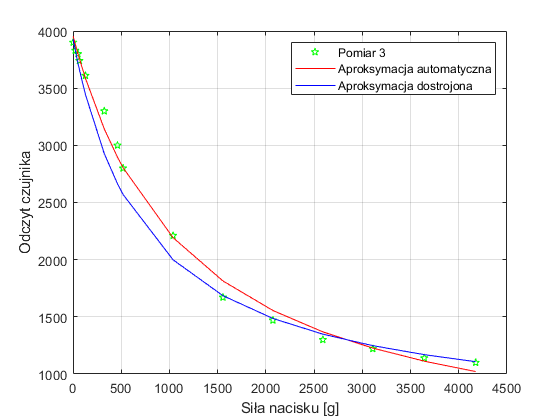
\includegraphics[width=0.85\linewidth]{img/badanie_1_aproksymacja.png}
    \caption{Aproksymacja wykonanych pomiarów hiperbolą}
    \label{f_badanie_1_aproksymacja}
\end{figure}

\begin{table}[!h]
\centering
\caption{Wyniki aproksymacji pomiarów pola czujnika}
\begin{tabular}{|l|r|r|r|r|}
\hline
Sposób aproksymacji       & \multicolumn{1}{c|}{$y$} & \multicolumn{1}{c|}{$a$} & \multicolumn{1}{c|}{$x_0$} & \multicolumn{1}{l|}{Błąd aproksymacji} \\ \hline
Automatyczna aproksymacja & 196                    & 4409590                & 1172                   & 286,4597                               \\ \hline
Ręczna aproksymacja       & 600                    & 2500000                & 750                    & 627,271                                \\ \hline
\end{tabular}
\label{t_badanie_1_aproksymacja}
\end{table}

\subsection{Pomiar podstawowych parametrów materiału nośnego}

Od tego momentu rozpoczęto wykonywać pomiary już bezpośrednio na materiale nośnym, a dokładniej złożeniu dwóch materiałów nośnych symulujących zbudowany gotowy czujnik. Do wykonania pomiarów opisanych w tym podrozdziale nie było konieczności budować specjalnego stanowiska pomiarowego. Były to pomiary podstawowych wartości, które można wykonać bez sprzętu laboratoryjnego. Pomiary te obejmowały:
\begin{itemize}
    \item masę czujnika,
    \item grubość czujnika,
    \item minimalny promień zgięcia materiału.
\end{itemize}

Jak można zauważyć, parametry te nie są kluczowe w wybranym zastosowaniu, ale mają kluczowe znaczenie, jeśli czujnik miałby być w przyszłości wykorzystywany na robotach posiadających dużą powierzchnię i~cała ta powierzchnia miałaby być pokryta sztuczną skórą. Wtedy wymienione wyżej parametry nabierają znaczenia, ponieważ wartości te odgrywają spore znaczenie w działaniu robota. Zwiększona masa ma negatywny wpływ na prędkość poruszania się robota oraz pobór energii potrzebnej do poruszania się, co~może skutkować np. znacznie krótszym czasie pracy na baterii. Większa masa sztucznej skóry utrudnia również zamocowanie jej na robocie i~wymaga do tego solidniejszych, bardziej skomplikowanych rozwiązań. Natomiast większa grubość czujnika powoduje, że robot zajmuje więcej przestrzeni, co może powodować większe prawdopodobieństwo wchodzenia w kolizje.

Jako pierwszy wykonany został pomiar grubości, który tak właściwie nie musiał być wykonywany, ponieważ posiadane próbki gumy miały grubość ustaloną przez producenta. 
Grubości warstwy taśmy miedzianej wynoszące $25\mu m$ \cite{b_site_kamami_tasma} każda oraz grubość folii Velostat wynosząca $0,1 mm$ \cite{b_site_kamami_folia} przy grubości dwóch warstw gumy wynoszącej w~najmniejszym przypadku $10 mm$ była znikoma. 
Przy grubości dwóch warstw gumy, wynoszącej w najmniejszym przypadku $10mm$, grubości warstw taśmy miedzianej wynoszące $25um$ każda \cite{b_site_kamami_tasma} oraz grubość folii Velostat wynosząca $0,1mm$ \cite{b_site_kamami_folia} były znikome.
Dokładna względna różnica grubości przy doliczeniu miedzi i folii Velostat wynosiła w tym przypadku $1,5\%$ i jest to największa możliwa do~osiągnięcia niedokładność. Z tego powodu pomiary grubości zostały wykonane poprzez dodanie grubości gum składających się na budowę danego czujnika.

Kolejną podstawową wartością łatwą do zmierzenia jest masa materiałów nośnych. Cały proces wymaga jedynie działającej wagi, kładzeniu na niej gotowych czujników i~odczycie pomiarów. Taka procedura została również wykonana w tym przypadku, podczas wykonywania tego pomiaru. Do pomiaru masy posłużyła ustawiona na równym podłożu waga kuchenna o zakresie pomiarowym $0-5000 g$ i dokładności $\pm 1g$. Wykorzystane stanowisko pomiarowe zostało przedstawione na rysunku \ref{f_badanie_2_stanowisko_waga}.

\begin{figure}[!h]
    \centering 
    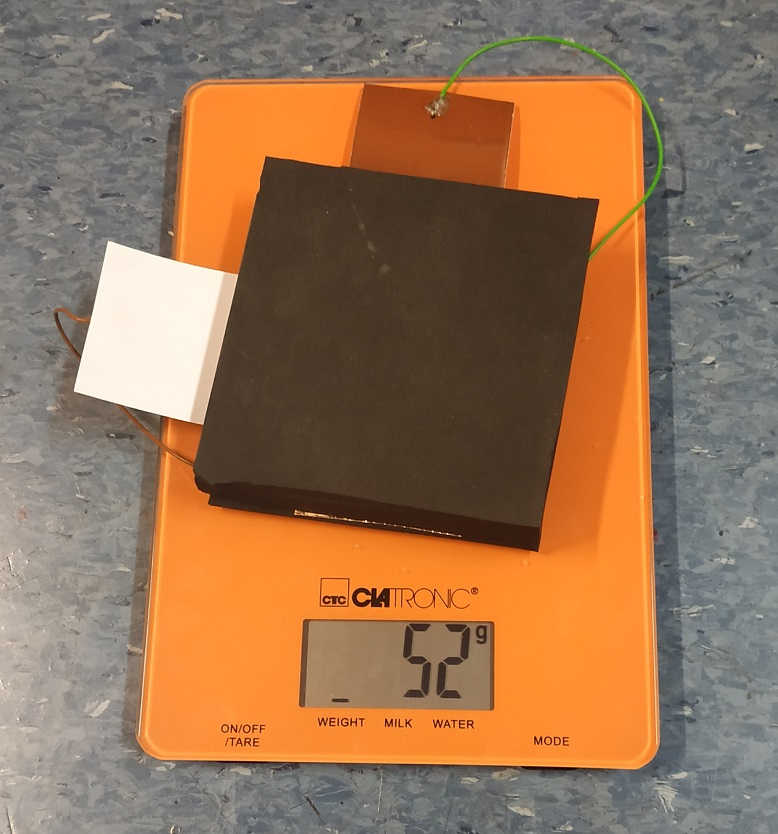
\includegraphics[width=0.5\linewidth]{img/badanie_2_stanowisko.jpg}
    \caption{Stanowisko pomiarowe do badania masy sztucznej skóry}
    \label{f_badanie_2_stanowisko_waga}
\end{figure}

Uzyskanie wartości wagi jest jeszcze możliwe na inny sposób - poprzez wyliczenie masy znając zajmowaną objętość czujnika oraz gęstość materiału użytego do jego budowy. Znając gęstość gumy NBR190, wynoszącą $190 \frac{kg}{m^3}$ oraz grubości poszczególnych warstw można skorzystać z przekształconego wzoru na gęstość:
\begin{equation}
    m = \rho*V
\end{equation}
Z tego wzoru można obliczyć masę użytego materiału nośnego, gdzie $m$ jest masą, $\rho$ gęstością, a $V$ objętością czujnika.

Zarówno wyniki pomiarów przy użyciu wagi, jak i obliczonych wartości zostały przedstawione w tabeli \ref{t_badanie_2_wyniki}. Widoczne różnice pomiędzy masą zmierzoną, a obliczoną są niewielkie i zazwyczaj wyższe wartości osiągają wartości zmierzone. Rozbieżności te mogą wynikać z niedokładnie przygotowanych pól czujnika oraz dodatkowo umieszczonych na gumie pasów folii miedzianej i okablowania zwiększających ich masę. Ponadto, w moim odczuciu waga kuchenna nie jest urządzeniem, w którym deklarowana przez producenta dokładność jest utrzymana w trakcie pomiaru i wyniki pomiarów otrzymane w ten sposób mają przez to większe niedokładności.

\begin{table}[!h]
\centering
\caption{Pomiar wagi testowanych materiałów nośnych}
\begin{tabular}{r|r|c|c}
\multicolumn{1}{l|}{\begin{tabular}[c]{@{}l@{}}Grubość górnej\\ warstwy {[}mm{]}\end{tabular}} & \multicolumn{1}{l|}{\begin{tabular}[c]{@{}l@{}}Grubość dolnej\\ warstwy {[}mm{]}\end{tabular}} & \multicolumn{1}{l|}{\begin{tabular}[c]{@{}l@{}}Waga zmierzona\\ {[}g{]}\end{tabular}} & \multicolumn{1}{l}{\begin{tabular}[c]{@{}l@{}}Waga obliczona\\ {[}g{]}\end{tabular}} \\
\hline
\hline
5                                                                                             & 5                                                                                             & 22                                                                                   & 19                                                                                   \\
5                                                                                             & 10                                                                                            & 33                                                                                   & 28,5                                                                                 \\
5                                                                                             & 15                                                                                            & 40                                                                                   & 38                                                                                   \\
5                                                                                             & 20                                                                                            & 52                                                                                   & 47,5                                                                                 \\
\hline
10                                                                                            & 5                                                                                             & 33                                                                                   & 28,5                                                                                 \\
10                                                                                            & 10                                                                                            & 45                                                                                   & 38                                                                                   \\
10                                                                                            & 15                                                                                            & 50                                                                                   & 47,5                                                                                 \\
10                                                                                            & 20                                                                                            & 61                                                                                   & 57                                                                                   \\
\hline
15                                                                                            & 5                                                                                             & 40                                                                                   & 38                                                                                   \\
15                                                                                            & 10                                                                                            & 50                                                                                   & 47,5                                                                                 \\
15                                                                                            & 15                                                                                            & 53                                                                                   & 57                                                                                   \\
15                                                                                            & 20                                                                                            & 65                                                                                   & 66,5                                                                                 \\
\hline
20                                                                                            & 5                                                                                             & 52                                                                                   & 47,5                                                                                 \\
20                                                                                            & 10                                                                                            & 61                                                                                   & 57                                                                                   \\
20                                                                                            & 15                                                                                            & 65                                                                                   & 66,5                                                                                 \\
20                                                                                            & 20                                                                                            & 77                                                                                   & 76                                                                                  
\end{tabular}
\label{t_badanie_2_wyniki}
\end{table}

Same wyniki są natomiast zgodnie z przewidywaniami mocno liniowe, a waga czujnika rośnie proporcjonalnie do grubości użytego czujnika. Pozwala to stwierdzić, że pod względem samej masy najlepszy jest najcieńszy czujnik.

Ostatnim z wykonanych pomiarów jest pomiar minimalnego promienia zgięcia. Minimalny promień zgięcia materiału jest najmniejszym promieniem łuku, który może przyjąć materiał bez jego przełamania, uszkodzenia lub zmniejszenia jego trwałości w sposób trwały lub na czas zgięcia. Przy zastosowaniu gumy jako warstwy nośnej sztucznej skóry ważne jest, aby wybrany materiał był w stanie jak najmocniej się zginać, by mógł on dopasować się do kształtu robota, a w szczególności jego rogów. W badanym przypadku nie jest to jednak krytyczne kryterium. Robot, na którym zostanie założona sztuczna skóra ma promienie gięcia obudowy równe $\sim 10mm$, co jest stosunkowo dużym promieniem. Sam czujnik nie zostanie jednak założony bezpośrednio na obudowę, tylko na specjalny szkielet, który nie będzie posiadał krzywizn o bardzo małym promieniu.

Wstępny pomiar minimalnego promienia gięcia wykonywany dłońmi wykazał jednak, że wszystkie wybrane do badań materiały pozwalają na ich zginanie na praktycznie zerowym promieniu bez widocznej utraty swoich właściwości. Powodem tego jest badanie gumy, która strukturalnie jest bardzo elastyczna.
Widoczna była jedynie różnica w sile potrzebnej, aby dany materiał doprowadzić do zgięcia z tak niewielkim promieniem. Dlatego wykonane pomiary nie opierały się ostatecznie na wykryciu minimalnego promienia zgięcia materiału, lecz na pomiarze siły potrzebnej do doprowadzenia materiału do tego samego promienia zgięcia.

Pomiary te zostały wykonane na stanowisku, gdzie fragment gumy został stabilnie zamocowany w imadle.
Pomiar siły potrzebnej do~osiągnięcia tej pozycji był wykonywany za pomocą siłomierza z zakresem pomiaru $0-100 N$ i dokładności $\pm 2 N$. 
Pomiar był wykonywany poprzez ściąganie gumy za pomocą siłomierza w dół, aż do momentu, kiedy guma owinęła się na konstrukcji imadła dotykając jego zewnętrznej części. W~tym momencie pobierany był pomiar siły.
Podczas pomiarów czasami miedziana taśma pękała, dlatego też większość pomiarów została wykonana na gumie bez naklejonej taśmy miedzianej, która nie ma żadnego wpływu na wynik tego pomiaru.
Stanowisko pomiarowe podczas wykonywania pomiaru zostało przedstawione na rysunku \ref{f_badanie_2_giecie}, a wyniki pomiarów w tabeli \ref{t_badanie_2_giecie}. 

\begin{table}[!h]
\centering
\caption{Pomiar siły potrzebnej do zgięcia gumy}
\begin{tabular}{r|c}
Grubość gumy {[}mm{]} & Zmierzona siła {[}N{]} \\
\hline
\hline
5                     & 2                      \\
\hline
10                    & 10                     \\
\hline
15                    & 24                     \\
\hline
20                    & 42                    
\end{tabular}
\label{t_badanie_2_giecie}
\end{table}

\begin{figure}[!h]
    \centering 
    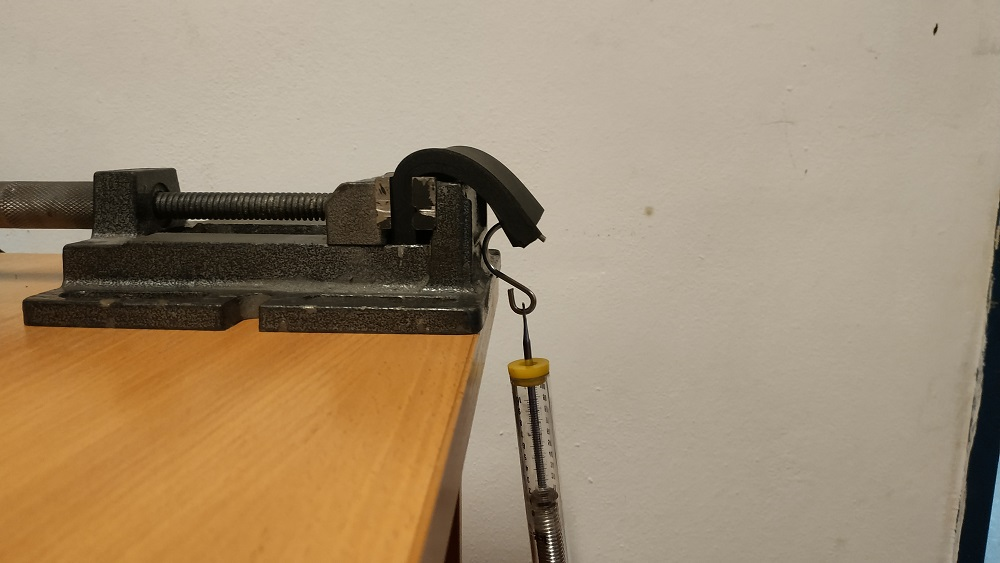
\includegraphics[width=0.9\linewidth]{img/badanie_gietkosc.jpg}
    \caption{Stanowisko pomiarowe siły wymaganej do zgięcia gumy}
    \label{f_badanie_2_giecie}
\end{figure}



Jak można zauważyć, chudsze warstwy gumy potrzebują użycia znacznie mniejszej siły do uzyskania wymaganego promienia zgięcia. Mimo iż potencjalnie każdy z materiałów nadaje się do użycia to te, które łatwiej się zginają są preferowane. Mniejsza siła potrzebna do zgięcia materiału umożliwia wykorzystanie do utrzymania jej w wymaganym kształcie lżejszych materiałów mocujących. Wykorzystanie dwustronnej taśmy klejącej jest prostszym i szybszym rozwiązaniem niż np. śrub, mimo iż taśma klejąca nie posiada tak samo dużej siły trzymania co śruby. Z tego powodu w tym teście również najlepsze do zastosowania okazują się być najcieńsze gumy.

Po analizie wyników można stwierdzić, że parametry mechaniczne jednoznacznie wskazują na to, że najlepszymi materiałami do wykorzystania są najcieńsze gumy. Posiadają one zarówno najmniejszą masę, najmniejszą grubość, jak i nie potrzeba wielkiej siły, aby doprowadzić je do zgięcia w~wymagany kształt.

\subsection{Badanie pochłanialności energii materiału nośnego}

Pochłanialność energii jest ważną cechą skóry. Odpowiada ona za znaczne zmniejszenie uszkodzeń zarówno robota, jak i otoczenia w wyniku uderzeń. Naturalnym jest, że~skóra powinna tłumić jak największą część energii otrzymywanego uderzenia.

Pomiar pochłanialności energii wykonany został przez upuszczanie na kolejne badane konfiguracje czujnika standardowej piłeczki golfowej, a następnie pomiar wysokości na jaką się ona odbijała. Wykorzystane do tego celu stanowisko pomiarowe zostało przedstawione na rysunku \ref{f_badanie_3_stanowisko}. Na rysunku \ref{f_badanie_3_stanowisko} widoczna jest przede wszystkim plansza z podziałką do~odczytu wysokości, na którą odbiła się upuszczana piłeczka. Plansza ta pozwalała na dokładny odczyt wartości z dokładnością do $\pm 5mm$, a pomiary o większej dokładności były szacowane (pozwalała na to jakość użytej kamery).

\begin{figure}[!h]
    \centering 
    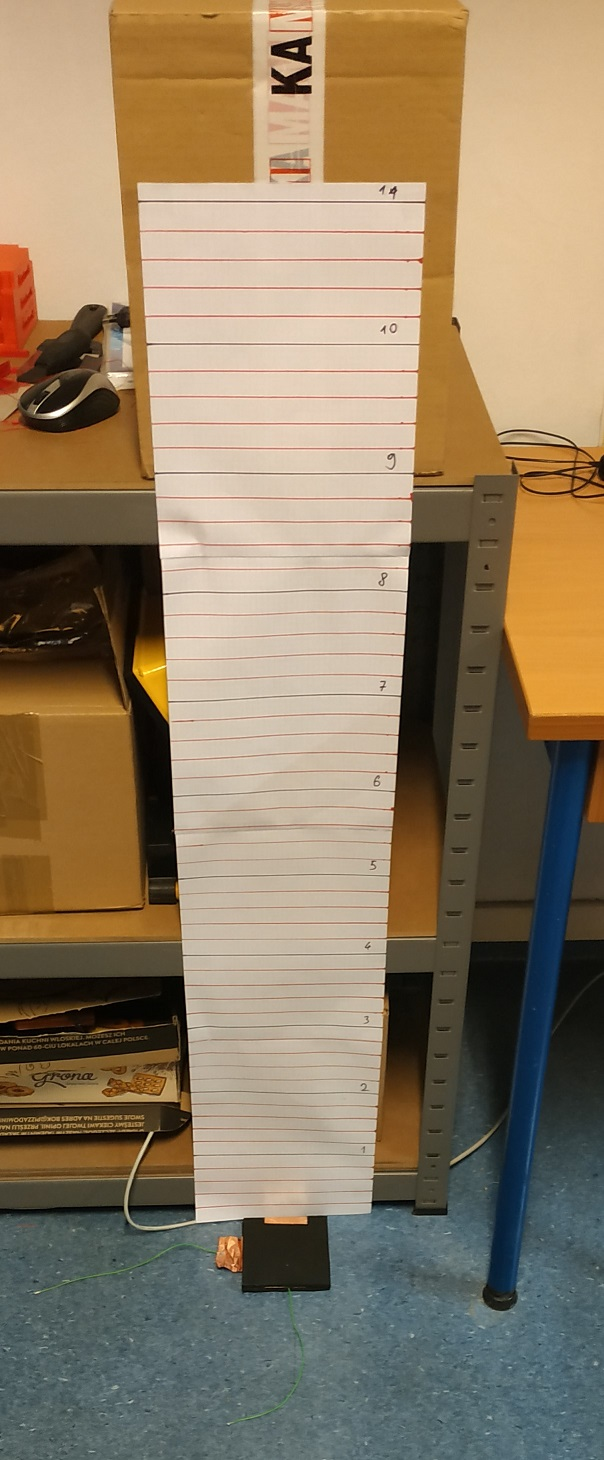
\includegraphics[width=0.3\linewidth]{img/badanie_3_stanowisko.jpg}
    \caption{Stanowisko pomiarowe do badania pochłanialności energii}
    \label{f_badanie_3_stanowisko}
\end{figure}

Aby móc dokładnie odczytywać wysokość, na którą odbiła się piłeczka golfowa została użyta szybka kamera, nagrywająca obraz w $100$ klatkach na sekundę w rozdzielczości $1280x720 px$. Odtworzenie nagranych testów pozwoliło poklatkowo bardzo dokładnie odczytać wysokość, na jaką wzniosła się piłeczka po odbiciu od badanego czujnika. Kamera była umieszczona w odległości $2000 mm$ od planszy, a~pomiary były dokonywane w~odległości $\sim 50 mm$ od planszy. W ten sposób zminimalizowano wpływ występującego przesunięcia kątowego i~upewniono się, że odczytane z obrazu wartości wysokości odbicia są jak najmniej zniekształcone. Oprócz pominięcia błędu kątowego pominięto również istniejące opory, w tym opór powietrza.

Piłeczka golfowa była zrzucana na czujnik z wysokości dokładnie $1000 mm$ nad powierzchnią czujnika. Oznacza to, że wysokość upuszczania piłeczki zmieniała się w~zależności od tego, jak gruby czujnik był badany. Pozwoliło to na otrzymanie danych, które~można porównywać pomiędzy czujnikami tylko poprzez odjęcie grubości czujnika od wysokości odbicia. Dlatego też wszystkie zaprezentowane w tej pracy wyniki uwzględniają wykonanie tego prostego obliczenia i zostały opisane jako względne - uwzględniając wysokość badanego czujnika. Każdy z wykonanych pomiarów został powtórzony przynajmniej 3 razy, a~uzyskany wynik - uśredniony.

Zanim przystąpiono do właściwych pomiarów wykonany został także pomiar tego, jaką część energii pochłania podłoże, na którym testowane były czujniki, aby uzyskać względną wartość o jaką tłumią zbudowane czujniki. Pomiar ten wykonany został analogicznie do opisanej powyżej metody, poprzez kilkukrotne upuszczenie piłeczki i obliczenie średniej wysokości odbicia. Otrzymano w ten sposób wartość $808,33 mm$ jako średnią wysokość odbicia, co przekłada się na pochłanialność energii równą $19,17 \%$. Wyniki procentowej pochłanialności energii testowanych czujników przyrównywane są do pomiarów pochłanialności podłoża właśnie, a nie do wysokości upuszczania piłeczki. Całość otrzymanych wyników przeprowadzonych badań widoczna jest w tabeli \ref{t_badanie_3_wyniki_2}. Największe uzyskane wartości pochłanialności zostały oznaczone kolorem zielonym, a najgorsze kolorem czerwonym. Wyniki rozciągające się pomiędzy tymi skrajnościami zostały oznaczone odpowiednio przechodzącymi przez barwę pomarańczową kolorami.

\begin{table}
\centering
\footnotesize
\caption{Wyniki pomiarów pochłanialności energii użytych gum}
\label{t_badanie_3_wyniki_2}
\begin{tabular}{|l|c|c|c|c|c|c|c|c|}
\hline
\begin{tabular}[c]{@{}l@{}}Grubość\\ dolnej\\ warstwy\\ {[}mm{]}\end{tabular} &
  \multicolumn{4}{l|}{5} &
  \multicolumn{4}{l|}{10} \\ \hline
\begin{tabular}[c]{@{}l@{}}Grubość\\ górnej\\ warstwy\\ {[}mm{]}\end{tabular} &
  \multicolumn{1}{l|}{5} &
  \multicolumn{1}{l|}{10} &
  \multicolumn{1}{l|}{15} &
  \multicolumn{1}{l|}{20} &
  \multicolumn{1}{l|}{5} &
  \multicolumn{1}{l|}{10} &
  \multicolumn{1}{l|}{15} &
  \multicolumn{1}{l|}{20} \\ \hline
 &
  80 &
  75 &
  98 &
  97 &
  65 &
  70 &
  85 &
  85  \\ \cline{2-9} 
 &
  72 &
  80 &
  101 &
  77 &
  72 &
  72 &
  87 &
  90 \\ \cline{2-9} 
 &
  75 &
  75 &
  102 &
  101 &
  75 &
  78 &
  87 &
  86 \\ \cline{2-9} 
 &
  77 &
  80 &
   &
  95 &
  73 &
  76 &
   &
  88 \\ \cline{2-9} 
 &
  82 &
  85 &
   &
  110 &
  72 &
   &
   &
   \\ \cline{2-9} 
\multirow{-6}{*}{\begin{tabular}[c]{@{}l@{}}Pomiary\\ względne\\ wysokości\\ odbicia\\ {[}mm{]}\end{tabular}} &
  90 &
  84 &
   &
  100 &
  82 &
   &
   &
   \\ \hline
\begin{tabular}[c]{@{}l@{}}Średnia\\ względna\\ wysokość\\ odbicia\end{tabular} &
  79,33 &
  79,83 &
  100,33 &
  96,67 &
  73,17 &
  74,00 &
  86,33 &
  87,25  \\ \hline
\begin{tabular}[c]{@{}l@{}}Pochłanialność\\ energii {[}\%{]}\end{tabular} &
  \cellcolor[HTML]{68EE2A}90,19 &
  \cellcolor[HTML]{70ED2D}90,12 &
  \cellcolor[HTML]{FF0803}87,59 &
  \cellcolor[HTML]{FF4721}88,04 &
  \cellcolor[HTML]{00FF00}90,95 &
  \cellcolor[HTML]{0EFC06}90,85 &
  \cellcolor[HTML]{DDDB59}89,32 &
  \cellcolor[HTML]{EDD95F}89,21 \\ \hline
\end{tabular}
\end{table}

\addtocounter{table}{-1}
\begin{table}
\centering
\footnotesize
\captionsetup{list=no}
\caption{ \textbf{(c.d.)} Wyniki pomiarów pochłanialności energii użytych gum}
\begin{tabular}{|l|c|c|c|c|c|c|c|c|}
\hline
\begin{tabular}[c]{@{}l@{}}Grubość\\ dolnej\\ warstwy\\ {[}mm{]}\end{tabular} &
  \multicolumn{4}{l|}{15} &
  \multicolumn{4}{l|}{20} \\ \hline
\begin{tabular}[c]{@{}l@{}}Grubość\\ górnej\\ warstwy\\ {[}mm{]}\end{tabular} &
  \multicolumn{1}{l|}{5} &
  \multicolumn{1}{l|}{10} &
  \multicolumn{1}{l|}{15} &
  \multicolumn{1}{l|}{20} &
  \multicolumn{1}{l|}{5} &
  \multicolumn{1}{l|}{10} &
  \multicolumn{1}{l|}{15} &
  \multicolumn{1}{l|}{20} \\ \hline
   &
  77 &
  83 &
  91 &
  94 &
  98 &
  91 &
  91 &
  98 \\ \cline{2-9} 
 &
  85 &
  90 &
  97 &
  89 &
  100 &
  89 &
  107 &
  99 \\ \cline{2-9} 
 &
  85 &
  78 &
  95 &
  99 &
  100 &
  94 &
  85 &
  101 \\ \cline{2-9} 
  &
  87 &
   &
  91 &
  86 &
  98 &
  84 &
  115 &
  100 \\ \cline{2-9} 
 &
   &
   &
   &
  95 &
  103 &
   &
  106 &
  101 \\ \cline{2-9} 
\multirow{-6}{*}{\begin{tabular}[c]{@{}l@{}}Pomiary\\ względne\\ wysokości\\ odbicia\\ {[}mm{]}\end{tabular}} &
    &
   &
   &
   &
  85 &
   &
   &
   \\ \hline
   \begin{tabular}[c]{@{}l@{}}Średnia\\ względna\\ wysokość\\ odbicia\end{tabular} &
  83,50 &
  83,67 &
  93,50 &
  92,60 &
  97,33 &
  89,50 &
  100,80 &
  99,80 \\ \hline
\begin{tabular}[c]{@{}l@{}}Pochłanialność\\ energii {[}\%{]}\end{tabular} &
  \cellcolor[HTML]{AEE346}89,67 &
  \cellcolor[HTML]{B1E247}89,65 &
  \cellcolor[HTML]{FF7D3B}88,43 &
  \cellcolor[HTML]{FF8D43}88,54 &
  \cellcolor[HTML]{FF3B1C}87,96 &
  \cellcolor[HTML]{FFC25C}88,93 &
  \cellcolor[HTML]{FF0000}87,53 &
  \cellcolor[HTML]{FF1108}87,65 \\ \hline
\end{tabular}
\end{table}

Po przeanalizowaniu danych można zauważyć, że wykorzystane czujniki niezależnie od użytych grubości gum dają podobne wartości wysokości odbicia. Wartości te mieszczą się w przedziale $73,17-100,80mm$. Pomimo tak podobnych wyników widoczne są również wyraźnie różnice pomiędzy użytymi grubościami gum. Czujnik osiągał dużo lepszą pochłanialność energii, kiedy jego górna warstwa była wykonana z gumy o grubości $5mm$ lub $10mm$, w~przeciwnym razie uzyskane wyniki były znacznie gorsze. Można zauważyć w ten sposób, że to górna warstwa czujnika ma większe znaczenie jeśli chodzi o~pochłanialność energii. Dolna warstwa również nie pozostaje bez znaczenia, ponieważ dla grubości powyżej $10mm$ badane czujniki osiągały niższą pochłanialność energii. Podsumowując, optymalne pod względem pochłanialności energii okazują się być sztuczne skóry zbudowane z gum o grubościach $5mm$ i $10mm$ w różnych konfiguracjach.

% \subsection{Badanie rozkładania energii wewnątrz pola czujnika}

% Badania były chaotyczne i przyprawiły mi kilka siwych włosów i nie tego rozdziału w pracy
% Ogólne wnioski:
% - generator liczb losowych
% - wszystkie pomiary wychodziły podobnie (guma nie rozprasza energii na boki prawie wcale)
% - każda fałdka na folii miedzianej wywalała wyniki w kosmos (i przyprawiała kolejny siwy włos)
% - pole powierzchni, jego kształt i ułożenie nad czujnikiem ma spore znaczenie
% - te chudsze chyba lepiej wychodziły

% Garść losowych wyników jest w img/screen_rozklad


% \FloatBarrier
\subsection{Podsumowanie wykonanych badań}

Na podstawie wyników badań zebranych w tabelach \ref{t_badanie_2_wyniki}, \ref{t_badanie_2_giecie} oraz \ref{t_badanie_3_wyniki_2} można zauważyć, że~najcieńsze dostępne gumy najlepiej nadają się do wykonania prototypu sztucznej skóry. Dominują one nad tymi grubszymi w każdym badanym w trakcie pracy aspekcie. Posiadają one lepsze własności mechaniczne oraz znacznie lepszą absorpcję energii uderzenia. Dlatego też do budowy prototypu wybrana została kombinacja grubości gum $10 mm$ oraz $5 mm$.
Zdecydowano się użyć takiej kombinacji, mimo iż kombinacja $5 mm$ oraz $5 mm$ wydaje się być lepsza, szczególnie patrząc na testy czysto mechaniczne. Głównym powodem był fakt, że skóra o grubości $15 mm$, może się wgiąć bardziej niż skóra o grubości $10 mm$. Mimo wybrania nienajlepszej możliwej konfiguracji nie jest ona dużo gorsza od optymalnej w~przewidywanym przypadku użycia.
Grubszą warstwę gumy przeznaczono jako warstwę wewnętrzna sztucznej skóry, a cieńszą jako zewnętrzną. Nie ma konkretnego powodu użycia ich takiej kolejności. Jedyną przesłanką jest fakt, że grubsza warstwa lepiej absorbowała uderzenia we wszystkich testowanych konfiguracjach.

\newpage
\section{Integracja sztucznej skóry z systemem robota}
\label{s_integracja}

\subsection{Środowisko pracy robota}

W testach został wykorzystany opisywany już w tej pracy robot Tiago, w konfiguracji bez dołączonych manipulatorów, lecz z uchwytem na tablet i czytnikiem NFC. Dodatkowo, do robota został dostawiony (położony na wierzchu robota) notebook z systemem Ubuntu 18.4 pozwalający w wygodny sposób obserwować i pracować na systemie ROS używanym przez robota. Został także dodany mikrofon dookolny o dużo lepszej jakości rejestrowanego dźwięku, niż ten wbudowany w robota. Mikrofon ten został podłączony bezpośrednio do notebooka. Został on także wykorzystany w innym projekcie w sterowaniu robotem za pomocą komend głosowych. Robot jest także podłączony do sieci WiFi i~przygotowany do pracy w~systemach IOT. Obecna konfiguracja robota, wraz z~dołączonymi peryferiami, została w~pełni przedstawiona na rysunku \ref{f_tiago_system} \cite{b_unpublic_system_lab}. 

\begin{figure}[!h]
    \centering 
    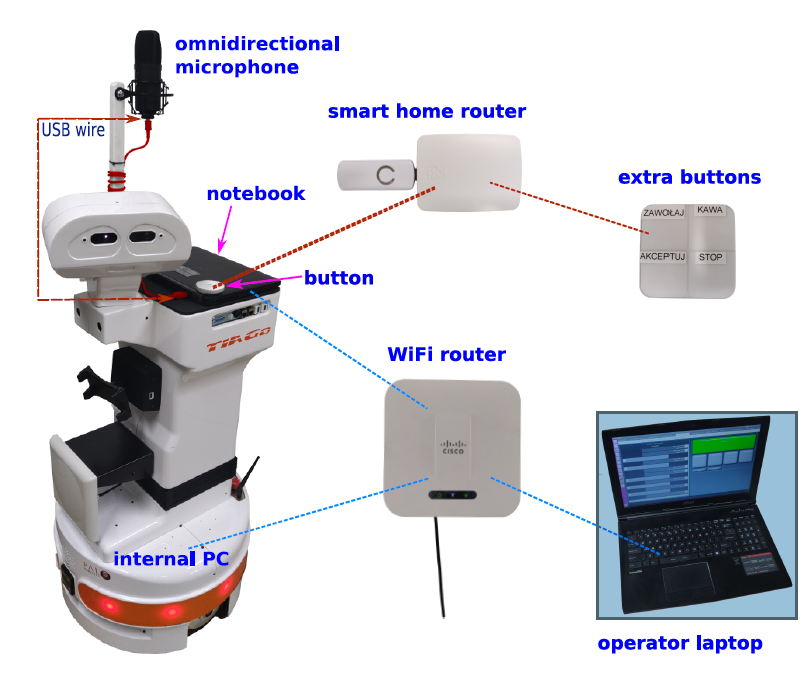
\includegraphics[width=0.9\linewidth]{img/tiago_system_lab.png}
    \caption{Robot Tiago wraz z dołączonym do niego systemem \cite{b_unpublic_system_lab}}
    \label{f_tiago_system}
\end{figure}

Tiago dostępny w laboratorium, podobnie jak jego symulacja, działa na systemie ROS w~wersji \textit{melodic}. W symulacji w dużej mierze wykorzystywane są pakiety dostarczane przez producenta - PAL Robotics, ale zostały obudowane przez dodatkowe pakiety zawierające m.in. mapę laboratorium robotycznego w~rzeczywistych wymiarach wraz z~odwzorowaniem przedmiotów znajdujących się w nim. Odwzorowane laboratorium w~programie Gazebo, wraz z~widocznym robotem, jest przedstawione na rysunku~\ref{f_lab_gazebo}. Widoczne na obrazku wyraźne niebieskie linie obrazują wiązki z~laserowego czujnika odległości i~skupiają się one przy robocie. 

\begin{figure}[!h]
    \centering 
    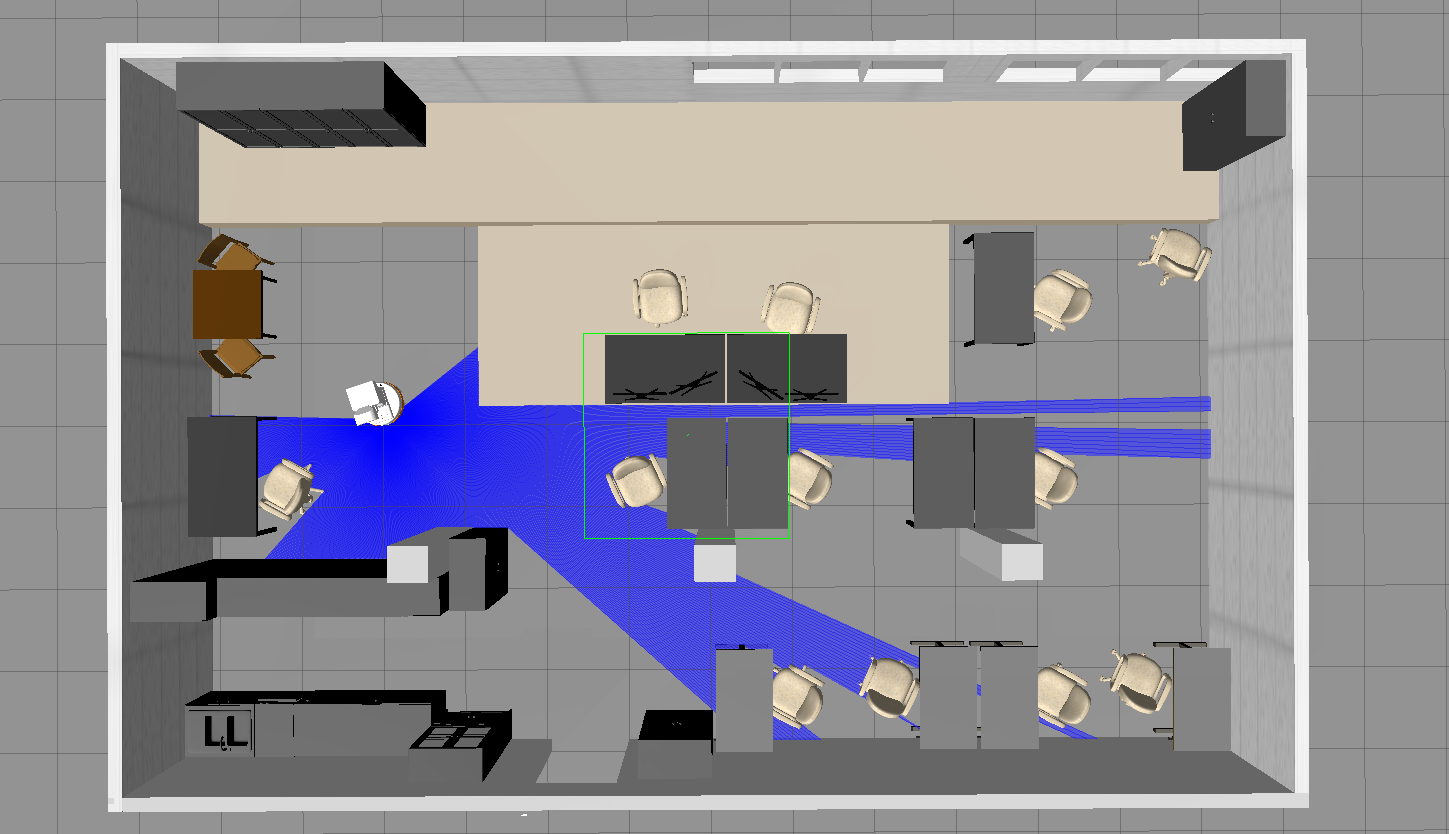
\includegraphics[width=0.95\linewidth]{img/ros_gazebo_lab.png}
    \caption{Laboratorium robotyczne odwzorowane w programie Gazebo}
    \label{f_lab_gazebo}
\end{figure}

\subsection{Budowa modułu sztucznej skóry mocowanego na robocie Tiago}
\label{ss_integracja_budowa}

Konstruowanie prototypu przeznaczonego do umieszczenia na robocie zostało zapoczątkowane przez dokładne zebranie wszystkich pomiarów z robota oraz zaplanowanie, jak projektowany czujnik będzie wyglądał. Zostało także wybrane dokładne umiejscowienie sztucznej skóry na robocie, jak również ustalono za ochronę których części będzie on odpowiadał. W ten sposób wywnioskowano, że czujnik powinien się znajdować w~górnej części robota. Tiago w~górnej części nie posiada żadnych czujników odległości i~jest bardziej narażony na przypadkowe uderzenia przez człowieka lub wiszące przedmioty. Czujnik planowo został zaprojektowany tylko do ochraniania tylnej i bocznych części robota. Przednia część nie była chroniona, ponieważ jest w niej umiejscowiona głowa, której ochrona wymaga użycia bardziej skomplikowanych kształtów czujnika. Użycie niewyprofilowanego czujnika wiązałoby się z sporym wyjściem poza istniejący obrys robota. Dodatkowo, zamontowany czujnik nie może w żaden sposób blokować ruchów głowy robota.

Szkielet sztucznej skóry zbudowany został z dociętej na wymiar płyty MDF o grubości $6 mm$. Jest to materiał lekki, o niewielkiej grubości, a jednocześnie wystarczająco sztywny, aby nie uginać się pod wpływem siły wywieranej na sztuczną skórę. Dodatkowymi plusami przemawiającymi za jego wyborem są duża dostępność, niska cena i bardzo łatwa obróbka.

% TODO zdjęcie szkieletu??

Do tak przygotowanego szkieletu przymocowana została za pomocą taśmy dwustronnej sztuczna skóra wykonana na wymiary szkieletu.
Kolejne warstwy sztucznej skóry zostały zbudowane z dobranej wcześniej gumy o grubości $10 mm$ przeznaczonej na warstwę wewnętrzną czujnika. Taśma dwustronna jest do jej zamocowania w pełni wystarczalna, z~powodu małej masy całego czujnika. Do warstwy wewnętrznej przymocowane zostały pionowe paski taśmy miedzianej o szerokości $25 mm$ z dolutowanymi w ich górnej części przewodami. Zastosowanie węższych pasków pozwala zwiększyć dokładność wykrywania kierunku, z którego wywierany jest nacisk. Do tak przygotowanej wewnętrznej warstwy doklejony został swobodnie zwisający kawałek folii Velostat. Swobodne ułożenie folii jest konieczne, ponieważ dowolne naprężenie folii zmniejsza jej rezystancję, co drastycznie wpływa na błędy w odczytywanych danych i~wprowadza duże zakłócenia. Do całości przymocowano również (taśmą dwustronną) zewnętrzny fragment gumy ochronnej o~grubości $5 mm$ z~przymocowanym do niego poziomym paskiem folii miedzianej o~szerokości $50 mm$. W tym przypadku pas folii miedzianej jest szerszy, ponieważ korzystając z~pojedynczego poziomego paska folii ważne jest, aby zbierał on  naciski z jak najszerszego obszaru. Zbudowany w~ten~sposób czujnik w opisywanej konfiguracji mocowanej na tył robota widoczny jest na zdjęciu \ref{f_szkielet_obity}.

\begin{figure}[!h]
  \begin{subfigure}[t]{0.5\linewidth}
    \centering
    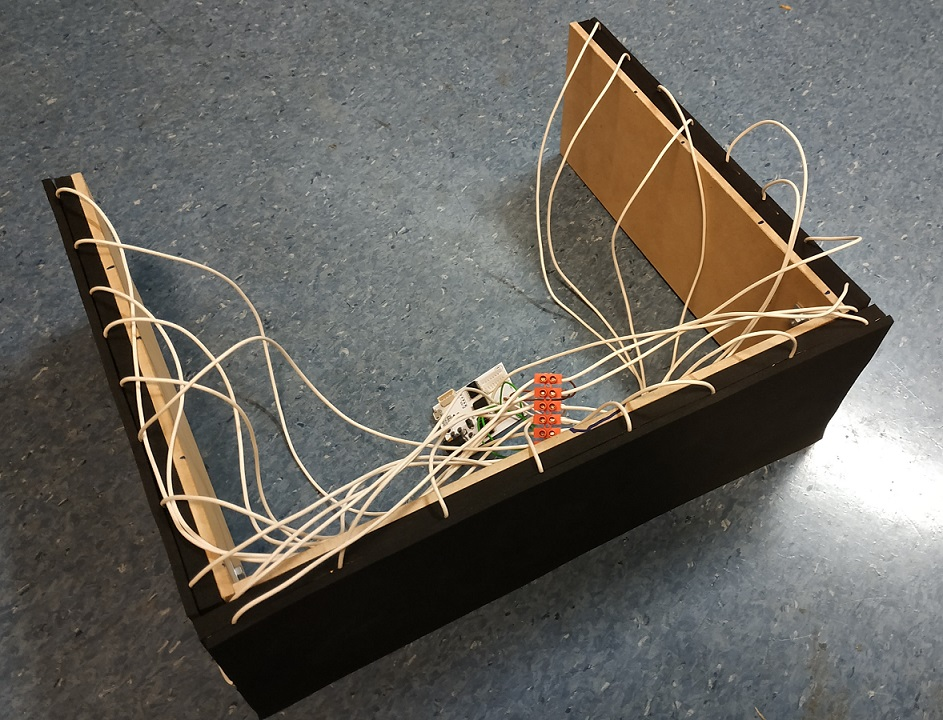
\includegraphics[width=0.85\linewidth]{img/szkielet_obity_przod.jpg} 
    \caption{Widok z zewnątrz prototypu} 
    % \vspace{4ex}
  \end{subfigure}%% 
  \begin{subfigure}[t]{0.487\linewidth}
    \centering
    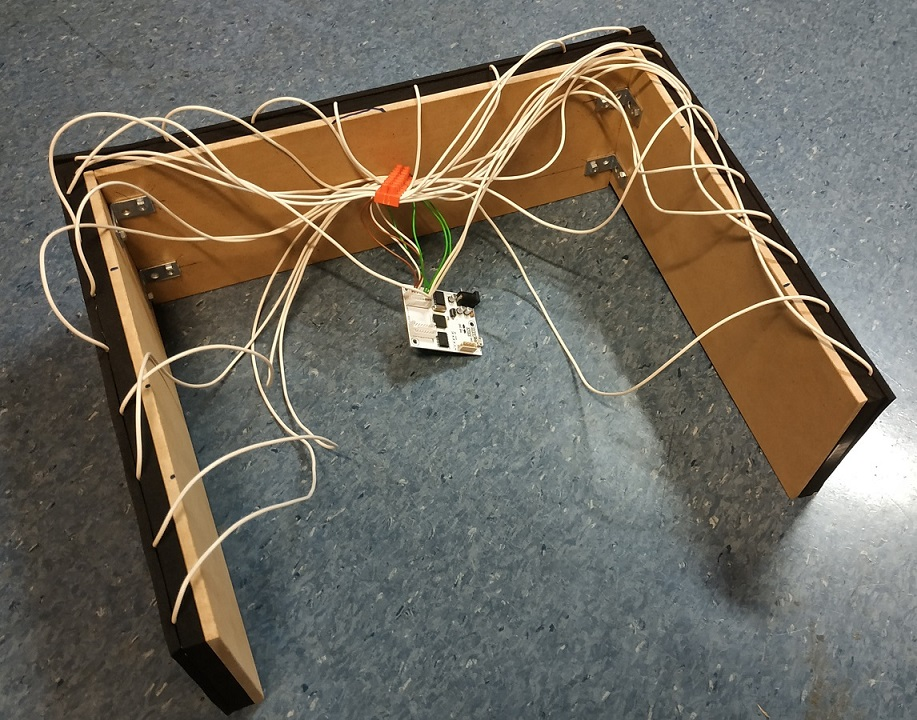
\includegraphics[width=0.85\linewidth]{img/szkielet_obity_tyl.jpg}
    \caption{Widok od wnętrza prototypu} 
    % \vspace{4ex}
  \end{subfigure}
  
  \centering
  \caption{Zbudowany prototyp przeznaczony do zamocowania na robocie}
  \label{f_szkielet_obity}
\end{figure}

Konfiguracja sztucznej skóry została wykonana analogicznie jak podczas testów opisywanych w sekcji \ref{sss_budowa_weryfikacja_algorytmu}. Został on skonfigurowany jako matryca posiadająca $8$ kluczy i~$3$~przetworniki ADC. Jest to wersja stabilniejsza i posiadająca mniejsze zakłócenia, niż~wersja odwrotna ($3$ klucze, $8$ ADC), która największe zakłócenia zbiera przez znaczne rozproszenie pola odczytu przetworników. Użyta konfiguracja w całości pozwala obsłużyć wykonany czujnik z $24$ polami, jak również pozwala je wygodnie pogrupować. W pełni rozpisana konfiguracja znajduje się w tabeli \ref{t_szkielet_config}. Założenie przyjęte przy doborze kątów zakładało, że środki ścianek bocznych szkieletu znajdują się na środku robota. Odległości zostały wszędzie ustawione na wartość $1$, ponieważ żadna ze stron nie była priorytetowana.

\begin{table}[!h]
\centering
\caption{Konfiguracja pól czujnika w wersji na tył}
\begin{tabular}{|l|l|rrr|}
\hline
\multicolumn{1}{|l|}{}     &                                   & \multicolumn{1}{c|}{Kolumna 1} & \multicolumn{1}{c|}{Kolumna 2} & \multicolumn{1}{c|}{Kolumna 3} \\
\hline  & \cellcolor[HTML]{C0C0C0}Kąt       & \cellcolor[HTML]{C0C0C0}309°  & \cellcolor[HTML]{C0C0C0}219°  & \cellcolor[HTML]{C0C0C0}129°  \\
\multirow{-2}{*}{Rząd 1} & \cellcolor[HTML]{EFEFEF}Odległość & \cellcolor[HTML]{EFEFEF}1   & \cellcolor[HTML]{EFEFEF}1   & \cellcolor[HTML]{EFEFEF}1   \\ 
    & \cellcolor[HTML]{C0C0C0}Kąt       & \cellcolor[HTML]{C0C0C0}298°  & \cellcolor[HTML]{C0C0C0}208°  & \cellcolor[HTML]{C0C0C0}118°  \\
\multirow{-2}{*}{Rząd 2} & \cellcolor[HTML]{EFEFEF}Odległość & \cellcolor[HTML]{EFEFEF}1   & \cellcolor[HTML]{EFEFEF}1   & \cellcolor[HTML]{EFEFEF}1   \\ 
    & \cellcolor[HTML]{C0C0C0}Kąt       & \cellcolor[HTML]{C0C0C0}287°  & \cellcolor[HTML]{C0C0C0}197°  & \cellcolor[HTML]{C0C0C0}107°  \\
\multirow{-2}{*}{Rząd 3} & \cellcolor[HTML]{EFEFEF}Odległość & \cellcolor[HTML]{EFEFEF}1   & \cellcolor[HTML]{EFEFEF}1   & \cellcolor[HTML]{EFEFEF}1   \\ 
    & \cellcolor[HTML]{C0C0C0}Kąt       & \cellcolor[HTML]{C0C0C0}276°  & \cellcolor[HTML]{C0C0C0}186°  & \cellcolor[HTML]{C0C0C0}96°   \\
\multirow{-2}{*}{Rząd 4} & \cellcolor[HTML]{EFEFEF}Odległość & \cellcolor[HTML]{EFEFEF}1   & \cellcolor[HTML]{EFEFEF}1   & \cellcolor[HTML]{EFEFEF}1   \\ 
    & \cellcolor[HTML]{C0C0C0}Kąt       & \cellcolor[HTML]{C0C0C0}264°  & \cellcolor[HTML]{C0C0C0}174°  & \cellcolor[HTML]{C0C0C0}84°   \\
\multirow{-2}{*}{Rząd 5} & \cellcolor[HTML]{EFEFEF}Odległość & \cellcolor[HTML]{EFEFEF}1   & \cellcolor[HTML]{EFEFEF}1   & \cellcolor[HTML]{EFEFEF}1   \\ 
    & \cellcolor[HTML]{C0C0C0}Kąt       & \cellcolor[HTML]{C0C0C0}253°  & \cellcolor[HTML]{C0C0C0}163°  & \cellcolor[HTML]{C0C0C0}73°   \\
\multirow{-2}{*}{Rząd 6} & \cellcolor[HTML]{EFEFEF}Odległość & \cellcolor[HTML]{EFEFEF}1   & \cellcolor[HTML]{EFEFEF}1   & \cellcolor[HTML]{EFEFEF}1   \\ 
    & \cellcolor[HTML]{C0C0C0}Kąt       & \cellcolor[HTML]{C0C0C0}242°  & \cellcolor[HTML]{C0C0C0}152°  & \cellcolor[HTML]{C0C0C0}62°   \\
\multirow{-2}{*}{Rząd 7} & \cellcolor[HTML]{EFEFEF}Odległość & \cellcolor[HTML]{EFEFEF}1   & \cellcolor[HTML]{EFEFEF}1   & \cellcolor[HTML]{EFEFEF}1   \\ 
    & \cellcolor[HTML]{C0C0C0}Kąt       & \cellcolor[HTML]{C0C0C0}231°  & \cellcolor[HTML]{C0C0C0}141°  & \cellcolor[HTML]{C0C0C0}51°   \\
\multirow{-2}{*}{Rząd 8} & \cellcolor[HTML]{EFEFEF}Odległość & \cellcolor[HTML]{EFEFEF}1   & \cellcolor[HTML]{EFEFEF}1   & \cellcolor[HTML]{EFEFEF}1  \\
\hline
\end{tabular}
\label{t_szkielet_config}
\end{table}

Testy wykonanej konfiguracji polegały na wywieraniu nacisku ręcznie i sprawdzania poprawności odczytów kąta oraz wynikowej siły nacisku odczytywanej przez czujnik. Ze~względu na~konieczność użytkowania czujnika w pozycji pionowej stabilne obciążenie obiektem jest niełatwe do zrealizowania. Testy polegające na sprawdzeniu poprawności identyfikacji naciskanych pól przebiegły w pełni pomyślnie. Problematyczny okazał się stan, w którym czujnik w ogóle nie był naciskany. Mimo braku nacisku czujnik wykrywał delikatny nacisk na praktycznie wszystkie pola. Skumulowanie tego błędu, dodatkowo zwiększone o brak czujników przedniej ścianki mogącej go niwelować, doprowadziło do otrzymania zwiększonych wartości siły w stanie spoczynku. Do rozwiązania tego problemu trzeba było zrewidować i poprawić konstrukcję mechaniczną czujnika (niektóre fragmenty folii Velostat okazały się delikatnie napięte). Wprowadzono także poprawki w~oprogramowaniu mikrokontrolera na nieuwzględnianie zaszumionych sygnałów. Dokładniejszy opis poprawek programistycznych został przedstawiony w rozdziale \ref{sss_budowa_opracowanie_algorytmu}. Finalnie po wykonaniu poprawek, czujnik podawał poprawne wartości w~momencie nacisku i~jego całkowity brak w momencie bezczynności.

\subsection{Integracja sztucznej skóry z robotem Tiago}
\label{ss_integracja_Python}

Integracja sztucznej skóry z Tiago rozpoczęła się od podłączenia skóry do symulatora. Aby wykonać interpretację odebranych ze sterownika informacji i przesłać polecenia ruchu bezpośrednio do robota został napisany węzeł ROS o nazwie $artificial\_skin$ przedstawiający dołączoną sztuczną skórę w systemie ROS. Węzeł ten został napisany w języku Python, który jest idealnym wyborem w momencie szybkiego prototypowania rozwiązań. Węzeł ten cały czas pobierał dane ze~sterownika i w momencie otrzymania kolejnej porcji danych obliczał prędkości wysyłane robotowi. Węzeł, oprócz odbierania danych ze~sztucznej skóry, odbierał także dane z czujnika laserowego robota nadawane na temacie $/scan\_raw$. Dane te także były wykorzystywane w algorytmie reakcji na nacisk robota, aby nie pozwolić robotowi uderzyć w otoczenie podczas odjeżdżania od źródła nacisku.

Węzeł sztucznej skóry wysyłał swoje pomiary na temacie $/key\_vel$. Temat ten przesyła dane typu $Twist$, które wyrażają prędkość liniową i kątową robota w przestrzeni \cite{b_site_ROS_twist}. Z~racji na posiadany przez Tiago różnicowy układ sterowania możliwa liczba kierunków ruchu jest mocno ograniczona \cite{b_site_tiago}. Układ różnicowy jest nieholonomiczny, ponieważ dwa koła odpowiadające za poruszanie się robota są ze sobą złączone sztywną osią. Przez tę niedogodność jedyne informacje wykorzystywane przez robota to zadana prędkość poruszania się w~osi~$x$ oraz prędkość obrotowa w~osi~$z$. Wybrany temat $/key\_vel$, na~którym wysyłane są prędkości, również nie został wybrany przypadkowo. Jest to temat wykorzystywany w~pierwotnej wersji do sterowania robotem z~klawiatury. Kanał ten posiada wysoki, ale nie najwyższy priorytet, to znaczy że sam jest ważniejszy niż kilka niektórych sygnałów sterujących, w~tym od~autonomicznej nawigacji, ale~sam także może zostać nadpisany przez np. sterowanie joystickiem. Struktura węzłowa robota w~symulacji wraz z~dołączoną sztuczną skórą została przedstawiona na rysunku \ref{f_struktura_ros_integracja}. Węzeł sztucznej skóry został wyróżniony kolorem czerwonym dla łatwiejszego zlokalizowania go.

\begin{figure}[!h]
    \centering 
    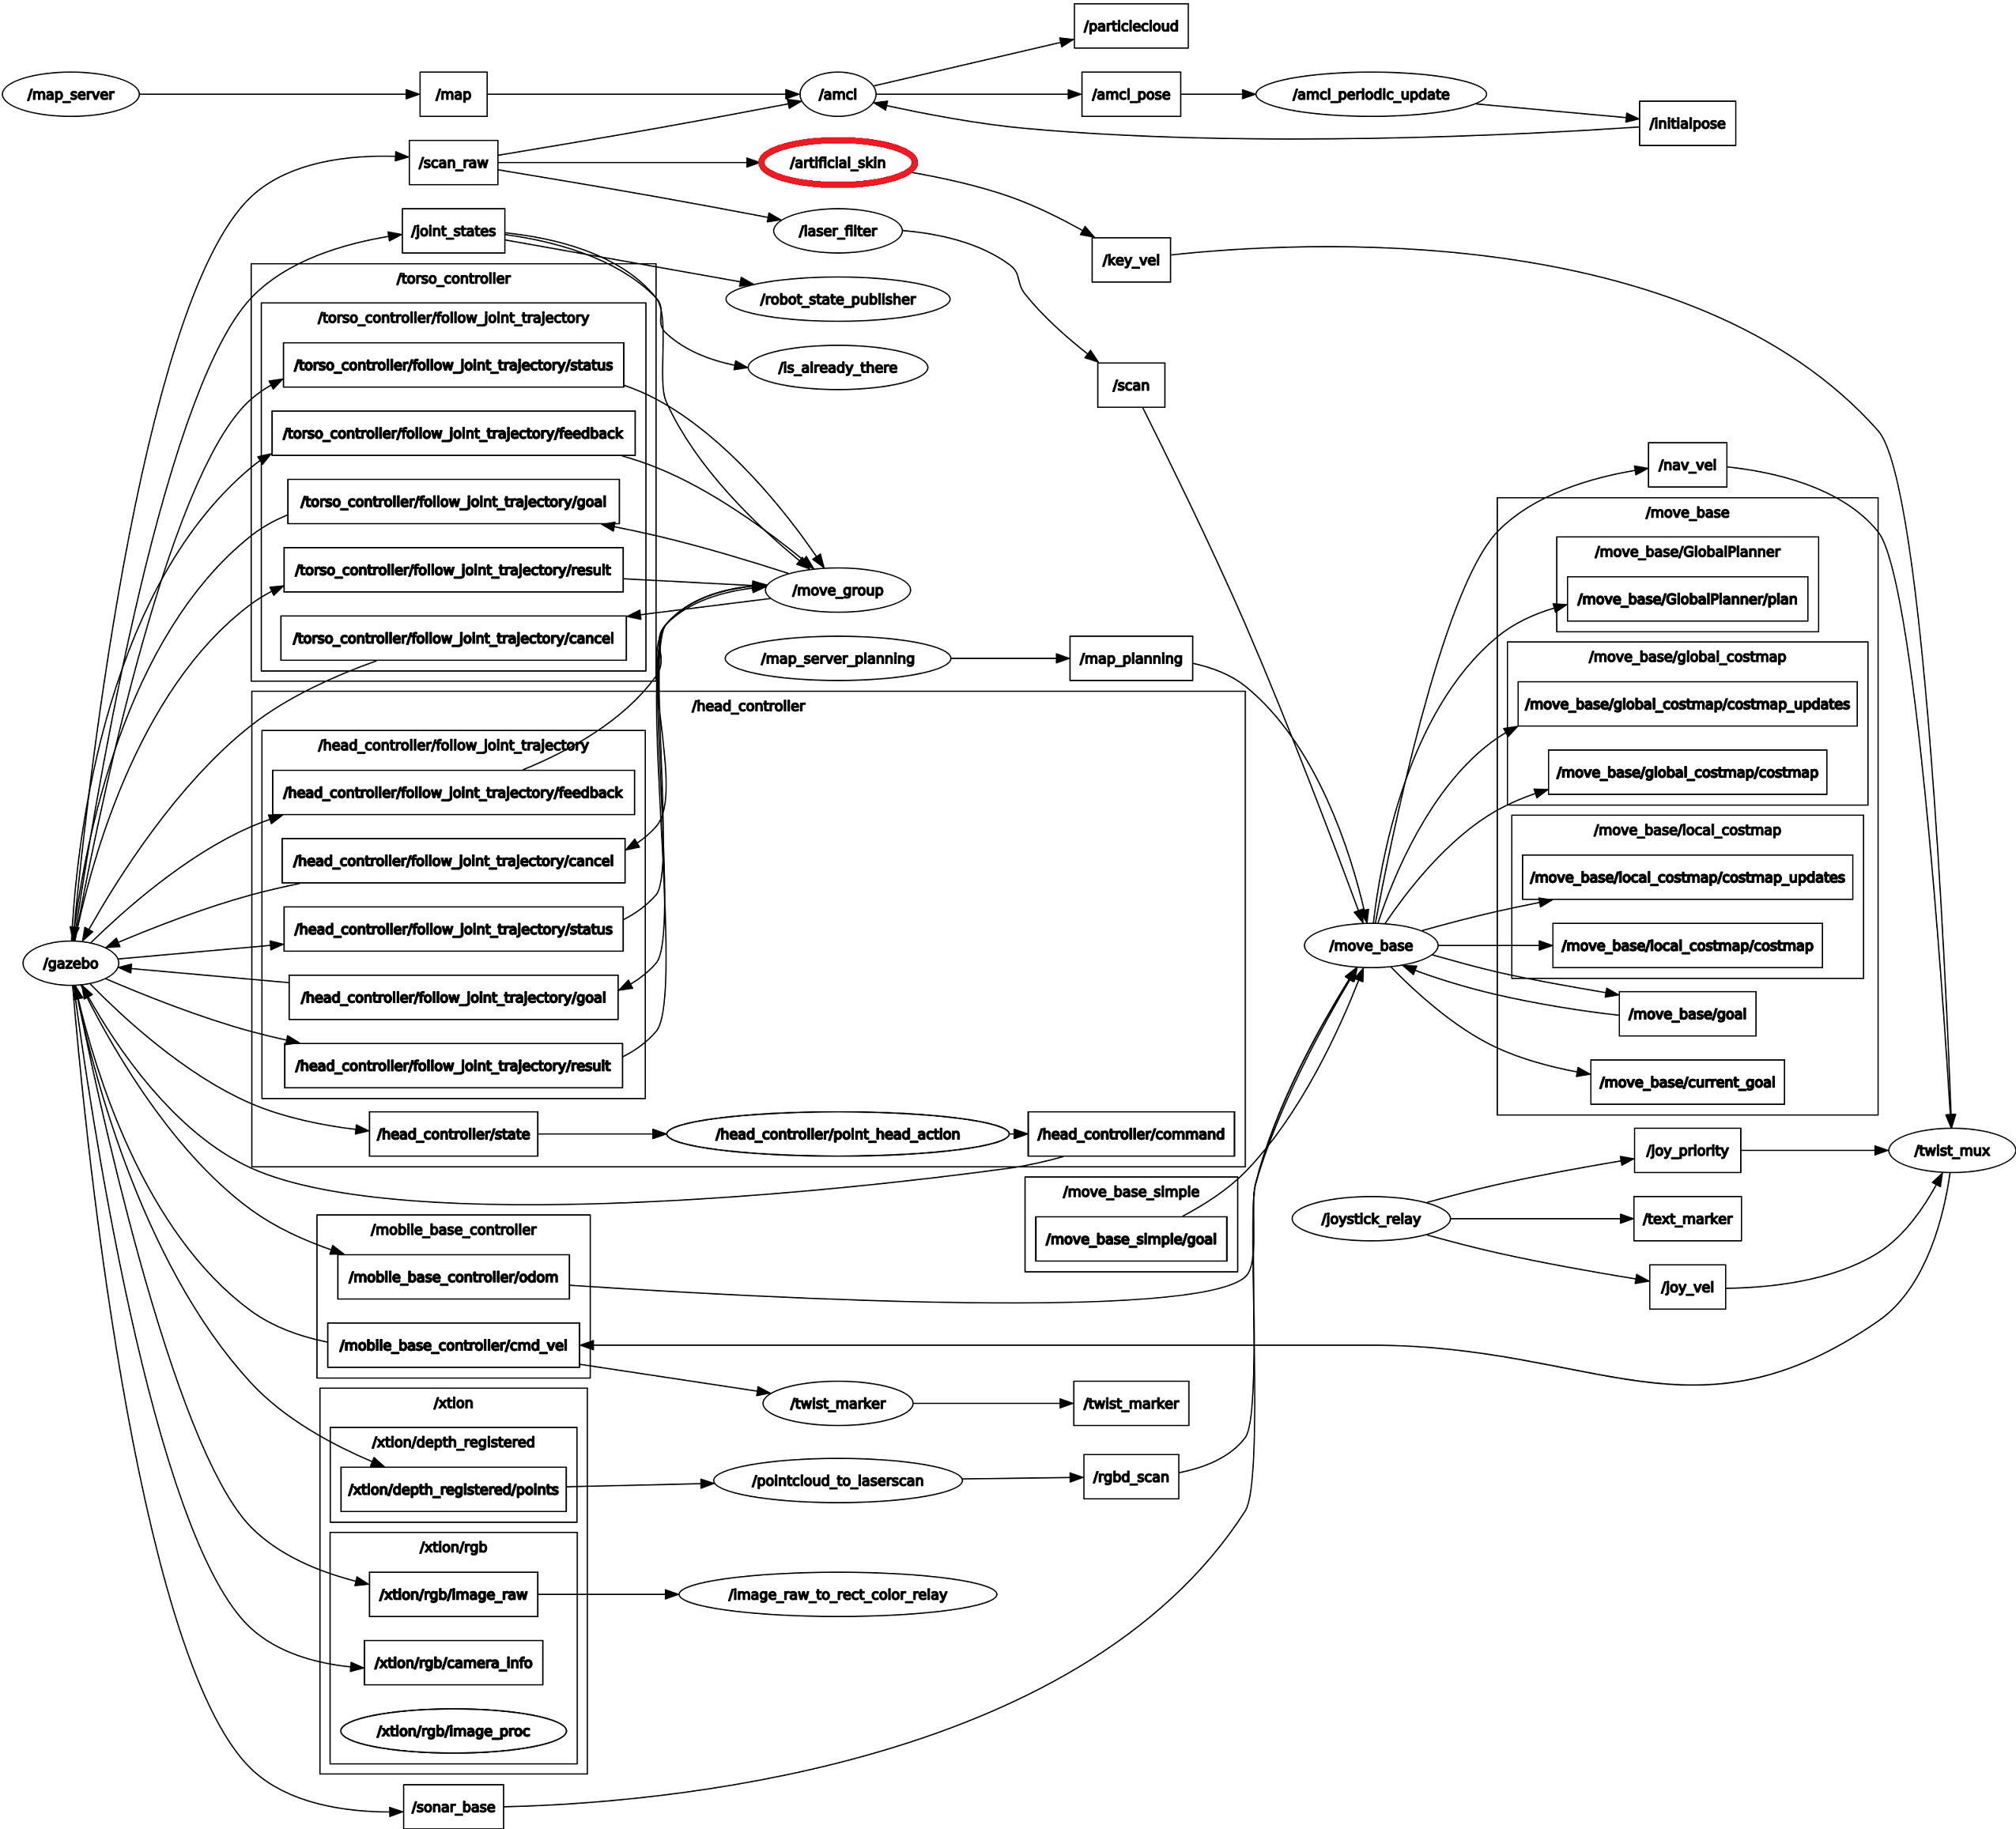
\includegraphics[width=1\linewidth]{img/ros_struktura.png}
    \caption{Struktura węzłowa robota Tiago wraz z dołączoną sztuczną skórą}
    \label{f_struktura_ros_integracja}
\end{figure}

% TODO zbieranie logów, czego xd

Integracja sztucznej skóry z robotem nastąpiła również pod względem mechanicznym. Została ona powieszona na robocie w górnej części, która jest trochę szersza niż tułów. Jako sposób mocowania zostały wybrane specjalnie zaprojektowane do tego celu i wydrukowane na drukarce 3D haczyki, które pozwalały na swobodne zakładanie i zdejmowanie modułu sztucznej skóry z robota. Sztuczna skóra została również podłączona do systemu za pomocą kabla USB łączącego ją z~notebookiem umieszczonym na robocie. Robot z~zamocowaną sztuczną skórą widoczny jest na rysunku \ref{f_czujnik_na_robocie}.

\begin{figure}
  \begin{subfigure}[t]{0.65\linewidth}
    \centering
    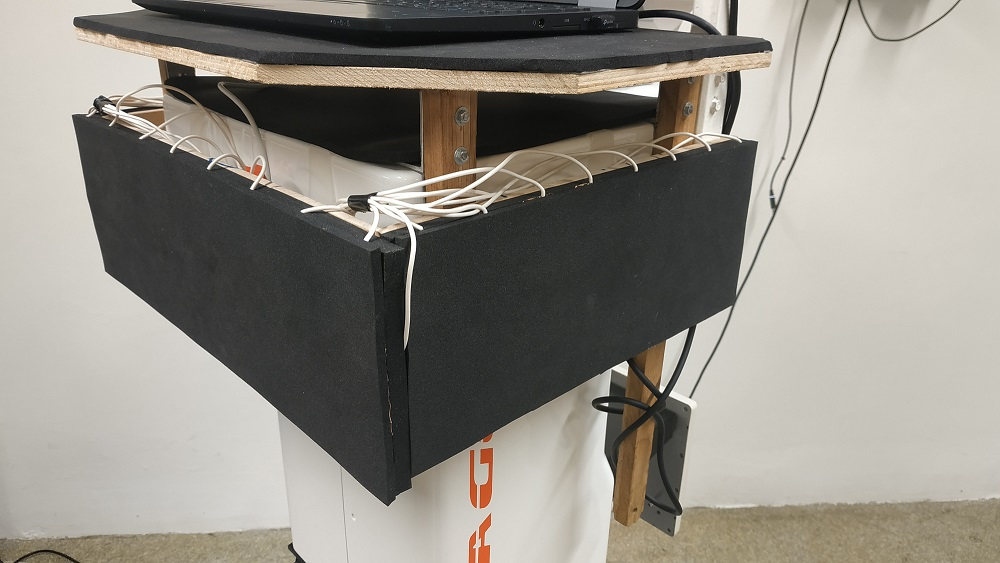
\includegraphics[width=0.9\linewidth]{img/czujnik_mocowanie_1.jpg} 
    \caption{Widok z bliska} 
    % \vspace{4ex}
  \end{subfigure}%% 
  \begin{subfigure}[t]{0.35\linewidth}
    \centering
    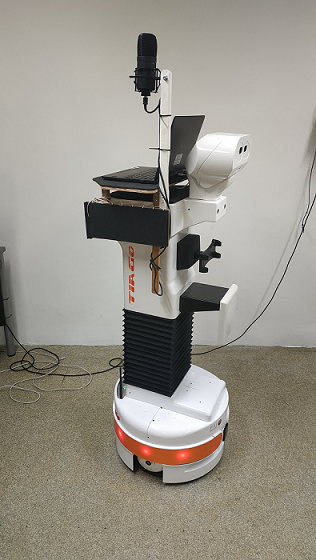
\includegraphics[width=0.9\linewidth]{img/czujnik_mocowanie_2.png}
    \caption{Widok całości robota} 
    % \vspace{4ex}
  \end{subfigure}
  \centering
  \caption{Zbudowany prototyp zamocowany na robocie}
  \label{f_czujnik_na_robocie}
\end{figure}

\subsection{Algorytm reakcji robota na wykryty nacisk}
\label{ss_integracja_algorytm}

Algorytm reakcji na nacisk jest jednym z kluczowych elementów w całym projekcie, zwieńcza on całe prowadzone badania. Ma on za zadanie interpretować przykładany nacisk i obliczać prędkość, z jaką poruszać się będzie robot. Podczas opracowywania algorytmu ściśle brano pod uwagę możliwości robota, a dokładniej ograniczenia, które nakłada różnicowy układ jezdny.

Opracowany algorytm wysyłający komendy sterowania uruchamiał się tylko w momencie, kiedy odczytane ze sterownika dane były niezerowe. Po otrzymaniu danych odczytana wartość siły jest przeliczana na lokalny mnożnik do wartości wystawianej na sterowaniu. Mnożnik ten jest uzyskiwany poprzez dzielenie otrzymanej siły pomiarów przez maksymalną wartość jaką sterownik może wysłać, czyli 10000 (a dokładniej 9999, ponieważ wartość siły jest zapisywana na 4 polach). % TODO w sumie to jest spierdolony kod napisałem
Dzięki temu prostemu zabiegowi odczytana wartość siły nie będzie się znajdowała w okolicach 1, czyli maksymalnej wartości jaka powinna być przesyłana do sterowania robota za pomocą tematu $/key\_vel$. Większe wysyłane wartości nie mają już żadnego wpływu na prędkość poruszania robota. Obliczony mnożnik jest podstawą do obliczenia siły ruchu, zarówno dla prędkości liniowej, jak i~obrotowej. Mnożnik ten został w trakcie testów doświadczalnie zmodyfikowany, ponieważ otrzymywane wartości okazały się zbyt niskie do płynnego sterowania robotem.

Dokładne ustalenie prędkości liniowej i kątowej zostaje obliczane na podstawie odczytanego kąta siły nacisku. Zastosowane podejście zostało pokazane na rysunku \ref{f_algorytm_kierunek_schemat}. Podstawą było odjeżdżanie robota w możliwy sposób od miejsca generującego nacisk.
Pokazane zachowanie zostało osiągnięte dzięki odpowiedniemu wykorzystaniu funkcji trygonometrycznych. W trakcie pierwszych testów okazało się, że wartości prędkości obrotowej robota są niewystarczające do satysfakcjonującego działania, dlatego zostały one dodatkowo zwiększone. Rozwiązanie to posiada pewne wady i istnieją momenty, w~których lepszym wyjściem jest zatrzymanie się, lecz jako propozycja działania prototypu zachowuje się dobrze.

\begin{figure}[!h]
    \centering 
    
\includegraphics[width=0.5\linewidth]{img/kierunek_shcemat.png}
    \caption{Podstawowy schemat działania robota jako reakcja na wykryty nacisk}
    \label{f_algorytm_kierunek_schemat}
\end{figure}

Wadą zaproponowanego rozwiązania może być obracanie się robota przy otrzymaniu nacisku z boku, powodując jeszcze trochę zwiększenie tego nacisku. Jednocześnie jednak część tego nacisku zostanie przełożona na tylną część robota i robot pojedzie do~przodu, a~z~racji iż wciąż się obraca odjedzie od przeszkody. Jest to spowodowane przez kwadratową obudowę czujnika, która w~praktyce nie jest równo odległa od środka obrotu robota. Jedynym rozwiązaniem, które pozwala na wyeliminowanie tego problemu jest wykorzystanie czujnika opartego na okręgu. Wykonanie czujnika okrągłego dostarcza jednak dodatkowych problemów konstrukcyjnych, a prototyp kwadratowy jest wystarczający do~pierwszych testów.

Dodatkowo do kodu zostało wprowadzone zabezpieczenie przed uderzeniem w obiekty znajdujące się przed robotem podczas odjeżdżania od wywieranego nacisku. Byłoby to niefortunne, gdyby robot próbując uciec od jednego naciskającego obiektu uderzył w~inny. Aby mieć możliwość interpretowania odległości, węzeł sztucznej skóry odczytuje informacje ze skanera laserowego na temacie $/scan\_raw$. Dane te są przesyłane w opakowanej formie w wiadomości typu $LaserScan$ i zawierają pełną informację o~odczytanych odległościach do obiektów w zakresie działania skanera, czyli $\ang{220}$ ($\pm \ang{110}$). Tak duży zasięg wydawał się być niepotrzebny, dlatego do dalszych obliczeń brane były pod uwagę tylko obiekty znajdujące się bezpośrednio przed robotem i częściowo po jego bokach. Ustalono również zakres wykorzystywanych pomiarów na $\ang{180}$ ($\pm \ang{90}$). Interpretacja pomiarów była bardzo prosta - jeśli zostanie odczytany dystans poniżej $0,4m$ to należy zatrzymać robota. Jednocześnie z zatrzymaniem, robot wciąż ma możliwość obracania się, a nawet jego mnożnik do prędkości obracania się zostaje po raz kolejny zwiększony, aby szybciej znaleźć kierunek, w którym robot może odjechać.

\newpage
\section{Weryfikacja działania sztucznej skóry na robocie}
\label{s_testy}

Końcowym etapem projektowania rozwiązania jest użycie go w rzeczywistości i~pomyślne przejście testów działania na robocie. Zanim jednak sztuczna skóra została założona na robota została ona przetestowana w~symulatorze Gazebo. Symulator ten, opisywany szerzej w~rozdziale \ref{ss_narzedzia_gazebo}, pozwala na przetestowanie działania i~algorytmów w~bezpiecznym środowisku.

\subsection{Weryfikacja działania w symulacji}

Weryfikacja działania czujnika zaczęła się od zainstalowania całego potrzebnego oprogramowania do jego obsługi wraz z paczkami robota Tiago i środowiskiem laboratoryjnym na maszynie wirtualnej z systemem Ubuntu 18.4. Po skonfigurowaniu wszystkich portów obsługujących USB stanowisko było gotowe do testowania.

\begin{figure}[!b]
    \centering 
    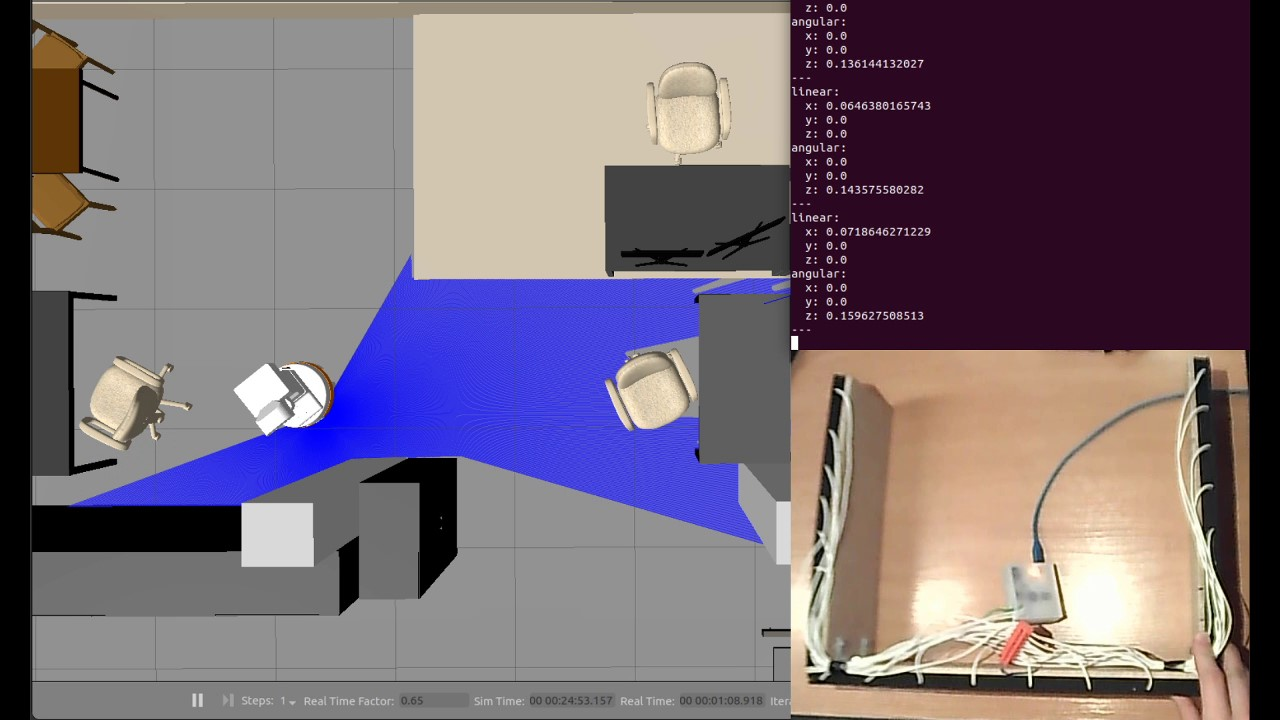
\includegraphics[width=0.95\linewidth]{img/test_gazebo.jpg}
    \caption{Test w symulatorze Gazebo wraz ze stanowiskiem i sygnałem sterującym}
    \label{f_test_gazebo}
\end{figure}

Same testy przebiegły sprawnie, wręcz bezproblemowo. Algorytm sterowania okazał się działać prawidłowo, jak również sterownik poprawnie przetwarzał i interpretował wywierany nacisk na skórę. Również część odpowiedzialna za zatrzymanie się robota przed przeszkodą prawidłowo działało. Testy w symulacji były jednak bardzo przydatne, ponieważ każda z opisanych działających funkcji została dokładniej dopracowana i dobrane zostały parametry jej działania. W sterowniku wyszła potrzeba wycięcia szumów i niskich wartości, ponieważ czujnik był niesymetryczny i sterował robotem nawet przy braku nacisku na skórę. Algorytm sterowania potrzebował dobrania poprawnych wartości wzmocnień sygnału, ponieważ te zastane nie pozwalały na płynną jazdę i obracanie się robota. Funkcja zatrzymywania się przed przeszkodą również potrzebowała lekkiego doregulowania w zakresie dystansu od przeszkody, w którym robot się zatrzymuje.

Nagranie wykonane podczas testów prezentujące jednocześnie widok symulatora Gazebo, dokładne sygnały sterujące przesyłane do robota na temacie $/key\_vel$ oraz aktualnie naciskane strefy czujnika umieszczone zostało w darmowym serwisie Vimeo \cite{b_site_vimeo_gazebo}. Screen z tego filmu został przedstawiony na rysunku \ref{f_test_gazebo}

\subsection{Weryfikacja działania na rzeczywistym robocie}

Po pomyślnej weryfikacji działania w symulacji, sztuczna skóra została zamocowana na robocie. Przejście pomiędzy tymi dwoma platformami okazało się bardzo proste. Jedyne, co było potrzebne, to podłączenie czujnika kablem USB bezpośrednio do gniazda, znajdującego się w notebooku połączonym z robotem Tiago. Po uprawnieniu do korzystania skryptu z~portu USB sztuczna skóra jest praktycznie gotowa do działania i~współpracy z~robotem.

\subsubsection{Pierwsza wersja sztucznej skóry - zakładana na tył}
Testy przeprowadzone na faktycznym robocie wykazały kilka znaczących różnic pomiędzy symulacją, a środowiskiem rzeczywistym. W trakcie testów niejednokrotnie zostały zaobserwowane zakłócenia, których nie było w symulacji. Najwieksza część wykrywanych zakłóceń pochodziła z sygnału otrzymywanego ze skanera laserowego. Otrzymywane dane posiadały czasami odczyty, które w żaden sposób nie pokrywały się ze stanem faktycznym - były całkowicie losowe. Regularnie wartości zmierzonej odległości okazywały się zbyt małe ($\sim 2mm$), aby pochodziły od jakiejkolwiek przeszkody. Pomiary te były błędnie interpretowane przez algorytm jako wykryta przeszkoda i praktycznie uniemożliwiały robotowi jakiekolwiek poruszanie się. Po odfiltrowaniu tych danych przez całkowite nieuwzględnianie ich (ponieważ są zbyt małe) zaobserwowano, że skaner laserowy ma również problem z odczytywaniem odległości w momencie kiedy w jego polu pojawiała się okrągła, metalowa noga stołu. Nie ma pewności jaka dokładnie była przyczyna tego zachowania, ale skaner laserowy czasami przesyłał mniejsze odległości, niż te występujące w~rzeczywistości. Mocno utrudniało to dojechanie do nogi stołu na odległość graniczną zapisaną w programie. W momencie, kiedy robotowi udało się dojechać do przeszkody to dalsze działania wykonywał już według ustalonego wcześniej algorytmu. Takiego zachowania nie zaobserwowano podczas testów robota na innych przeszkodach jak ściana czy krzesła.

Ważne było także ciągłe uważanie na zachowanie robota, czy samoczynnie nie wykonuje niepożądanych lub niebezpiecznych ruchów. Podczas wykonywanych prac nie zaobserwowano takich zachowań, ale w razie ich wystąpienia cały czas była osoba gotowa do naciśnięcia przycisku awaryjnego, znajdującego się u podstawy robota. Ewentualne nieopanowanie robota wiązałoby się z potencjalnie sporymi stratami materialnymi. Dlatego też użyte algorytmy zostały wcześniej pomyślnie przetestowane w symulacji. Robot w trakcie testów został przedstawiony na rysunku \ref{f_test_robot_1}.

\begin{figure}[!h]
    \centering 
    \includegraphics[width=0.95\linewidth]{img/test_robot_1.jpg}
    \caption{Robot Tiago podczas testów}
    \label{f_test_robot_1}
\end{figure}

Podczas użytkowania i sprawdzania poprawności zaimplementowanych rozwiązań wzięto pod uwagę kilka dodatkowych nieznacznych poprawek. Poza zaszumionym sygnałem otrzymywanym ze skanera laserowego okazało się także, że nie ma on zasięgu $\ang{220}$, jak~w~symulatorze, tylko $\ang{190}$ ($\pm\ang{95}$). Zostały także ustawione inne dopuszczalne odległości robota do przedmiotów. Wartość ta została zmniejszona z $40cm$ do $30cm$. Poza tymi małymi poprawkami kod przeniesiony z symulatora od razu nadawał się do korzystania z~robota.

Podczas używania prototypu wykonano kilka podstawowych testów jego działania. Pierwszy i podstawowy test polegał na sterowaniu robotem za pomocą naciskania na różne obszary sztucznej skóry. Test ten został wykonany pomyślnie i bez większych problemów. Został także wykonany, opisywany już wcześniej, test współpracy ze skanerem laserowym, gdzie sam program działał dobrze, lecz czujnik odległości czasami wysyłał błędne dane. Zostały też wykonane testy zachowania robota na uderzenia i statyczny nacisk. Test~działania na uderzenie przebiegł całkiem pomyślnie. Należy jednak zauważyć, że~to~czujnik przyjął większą część siły uderzenia, a sam robot odjechał dopiero po chwili. Testy~wykonane na statycznym nacisku (przedmiotem, który nie zmienia swojego położenia w czasie) pokazały niestety sporą wadę wykonanego czujnika - jego kształt. Zaprojektowany kształt posiadający kąty ostre powodował, że~w~pierwszej fazie, przy próbie obrotu robot mocniej naciskał na statyczny przedmiot, a nie jak zakładano zmniejszał ten nacisk. Jest to ogólny problem mocno związany z~napędem różnicowym robota, który przed jazdą w przód musi się najpierw cały obrócić. Nagranie z~wykonanych na robocie testów dostępne jest na serwisie Vimeo \cite{b_site_vimeo_kwadrat}.

\subsubsection{Finalna wersja sztucznej skóry - dookolna}

Testy wykonane na pierwszej wersji sztucznej skóry, wykazały jeden kluczowy błąd, który wynikał z użytego kształtu szkieletu. Niestety ta wada powodowała, że rozwiązanie nie spełniało jednego z głównych założeń sztucznej skóry - nie wywierania siły na środowisko. W momencie wykrywania nacisku z boku i obracania się w miejscu, robot wywoływał jeszcze większy nacisk na środowisko. Było to powodem budowy drugiej wersji sztucznej skóry opartej na okrągłym szkielecie, który pozbawiony jest tej wady.

Cała konstrukcja, poza częścią mechaniczną, pozostała dokładnie taka sama. Kolejne warstwy sztucznej skóry również zostały złożone w tej samej kolejności. Zmodyfikowana została tylko konfiguracja pól czujnika. 

Do budowy szkieletu wykorzystana została obręcz rowerowa $26" (1.5/559)$ o szerokości $2.5 cm$. Zewnętrzna część tej obręczy ma minimalnie większy obwód niż dolny obwód robota Tiago, dzięki czemu wykonany na nim czujnik nie zwiększy znacząco całkowitego promienia, który robot zajmuje w środowisku. Na zewnętrznej części obręczy zamocowana została za pomocą nitów blacha ocynkowana $0.5 mm$ o szerokości $120 mm$. Blacha ta zapewnia odpowiedni kompromis pomiędzy sztywnością konstrukcji, a pochłanianiem siły uderzeń. Do blachy zostały przyklejone taśmą montażową kolejne warstwy sztucznej skóry w sposób identyczny, jak opisany w rozdziale \ref{ss_integracja_budowa}.
Zbudowany szkielet został zamocowany do robota Tiago za pomocą lekkich listew drewnianych, śrub i wkrętów. 
Wykonanie takiej konstrukcji w pełni spełnia wymagania warstwy mechanicznej opisanej w rozdziale \ref{ss_budowa_mech}. Postępy prac nad budową drugiej wersji prototypu zostały przedstawione na rysunku \ref{f_test_prace_1}, a~zbudowany prototyp na rysunku \ref{f_test_ready_1}. Prototyp ten składa się z~$32$~pól sensorycznych, które są równomiernie rozłożone na całym okręgu, z~dodaniem $8$~pól, na~których nie ma umieszczonego czujnika. 
Obecność kilku pól bez czujnika wynika z~faktu, że~nie mógł on zostać tam zamocowany z~powodu łączenia się poziomych odcinków folii miedzianej oraz fizycznych ograniczeń sterownika. Wspomniana nowa konfiguracja sztucznej skóry została przedstawiona w~tabeli \ref{t_test_2_config}.

\begin{figure}[!h]
    \centering 
    \includegraphics[width=0.95\linewidth]{img/test_okr_prace_1.jpg}
    \caption{Postęp prac prowadzonych nad drugim prototypem sztucznej skóry}
    \label{f_test_prace_1}
\end{figure}

\begin{table}[!h]
\centering
\caption{Konfiguracja pól czujnika drugiej wersji sztucznej skóry}
\begin{tabular}{|l|l|rrrr|}
\hline
\rowcolor[HTML]{FFFFFF} 
 &
   &
  \multicolumn{1}{l|}{\cellcolor[HTML]{FFFFFF}Kolumna 1} &
  \multicolumn{1}{l|}{\cellcolor[HTML]{FFFFFF}Kolumna 2} &
  \multicolumn{1}{l|}{\cellcolor[HTML]{FFFFFF}Kolumna 3} &
  \multicolumn{1}{l|}{\cellcolor[HTML]{FFFFFF}Kolumna 4} \\ \hline
\rowcolor[HTML]{C0C0C0} 
\cellcolor[HTML]{FFFFFF}                         & Kąt       & 0° &90° & 180°  & 270°  \\ \cline{2-2}
\rowcolor[HTML]{EFEFEF} 
\multirow{-2}{*}{\cellcolor[HTML]{FFFFFF}Rząd 1} & Odległość & 1    & 1    & 1    & 1     \\ \cline{1-2}
\rowcolor[HTML]{C0C0C0} 
\cellcolor[HTML]{FFFFFF}                         & Kąt       & 9° & 99° & 189°  & 279°  \\ \cline{2-2}
\rowcolor[HTML]{EFEFEF} 
\multirow{-2}{*}{\cellcolor[HTML]{FFFFFF}Rząd 2} & Odległość & 1    & 1    & 1    & 1   \\ \cline{1-2}
\rowcolor[HTML]{C0C0C0} 
\cellcolor[HTML]{FFFFFF}                         & Kąt       & 18° & 108° & 198°  & 288°  \\ \cline{2-2}
\rowcolor[HTML]{EFEFEF} 
\multirow{-2}{*}{\cellcolor[HTML]{FFFFFF}Rząd 3} & Odległość & 1    & 1    & 1    & 1     \\ \cline{1-2}
\rowcolor[HTML]{C0C0C0} 
\cellcolor[HTML]{FFFFFF}                         & Kąt       & 27° & 117° & 207°  & 297° \\ \cline{2-2}
\rowcolor[HTML]{EFEFEF} 
\multirow{-2}{*}{\cellcolor[HTML]{FFFFFF}Rząd 4} & Odległość & 1    & 1    &1    & 1    \\ \cline{1-2}
\rowcolor[HTML]{C0C0C0} 
\cellcolor[HTML]{FFFFFF}                         & Kąt       & 45° & 135° & 225° & 315°\\ \cline{2-2}
\rowcolor[HTML]{EFEFEF} 
\multirow{-2}{*}{\cellcolor[HTML]{FFFFFF}Rząd 5} & Odległość & 1    & 1    & 1    & 1     \\ \cline{1-2}
\rowcolor[HTML]{C0C0C0} 
\cellcolor[HTML]{FFFFFF}                         & Kąt       & 54° & 144° & 234°  & 324°  \\ \cline{2-2}
\rowcolor[HTML]{EFEFEF} 
\multirow{-2}{*}{\cellcolor[HTML]{FFFFFF}Rząd 6} & Odległość & 1    & 1    & 1    & 1     \\ \cline{1-2}
\rowcolor[HTML]{C0C0C0} 
\cellcolor[HTML]{FFFFFF}                         & Kąt       & 63° & 153° & 243° & 333° \\ \cline{2-2}
\rowcolor[HTML]{EFEFEF} 
\multirow{-2}{*}{\cellcolor[HTML]{FFFFFF}Rząd 7} & Odległość & 1    & 1    & 1    & 1     \\ \cline{1-2}
\rowcolor[HTML]{C0C0C0} 
\cellcolor[HTML]{FFFFFF}                         & Kąt       & 72° & 162° & 252°  & 342°  \\ \cline{2-2}
\rowcolor[HTML]{EFEFEF} 
\multirow{-2}{*}{\cellcolor[HTML]{FFFFFF}Rząd 8} & Odległość & 1    & 1    & 1    & 1     \\ \cline{1-2}
\hline
\end{tabular}
\label{t_test_2_config}
\end{table}

Zbudowana sztuczna skóra od razu po okablowaniu i~wgraniu nowej konfiguracji była gotowa do działania. Z~uwagi na to, że algorytm sterowania został wcześniej przetestowany na robocie i~działał poprawnie, zrezygnowano z~testów drugiego prototypu w symulatorze Gazebo i~od razu przystąpiono do testów na robocie. Algorytm pomimo już poprawnego wcześniej działania został dodatkowo usprawniony poprzez dodanie do niego dobranej doświadczalnie rampy na sterowaniu prędkością, zarówno jazdy, jak i~obracania się. Rampa~ta została zaimplementowana w~celu złagodzenia bardzo gwałtownych skoków robota spowodowanych wykryciem nacisku na sztuczną skórę, widocznych wyraźnie podczas poprzednich testów. Minusem takiego podejścia jest wyraźne zwiększenie się czasu, jaki~Tiago potrzebuje, aby~odjechać od źródła kolizji.

\begin{figure}[!h]
    \centering 
    \includegraphics[width=0.95\linewidth]{img/test_okr_ready_2.jpg}
    \caption{Druga wersja prototypowej sztucznej skóry}
    \label{f_test_ready_1}
\end{figure}

Przeprowadzone testy obejmowały podobny zakres co testy pierwszego prototypu. Pierwszy test polegał na teście pracy i zachowania robota pod wpływem generowania nacisku na różnych częściach sztucznej skóry. Test przebiegł pozytywnie, a odczucia były lepsze niż w przypadku pierwszego prototypu. Zachowanie robota wydawało się lepiej odzwierciedlać miejsce, w którym robot był naciskany. Szczególnie mocno zauważalne było użycie rampy na sygnale sterującym, które spowodowało widoczne upłynnienie ruchów robota i zniwelowanie wykonywanych przez niego wcześniej szarpnięć. Dzięki nowej konstrukcji zaistniała także możliwość przetestowania reakcji Tiago na nacisk z~przodu robota, czego nie dało się wykonać w poprzedniej konstrukcji. Kolejnym testem był test współpracy sztucznej skóry z czujnikiem odległości. Przyniósł on tak samo dobre wyniki jak poprzednia iteracja sensora. 

Ostatnim z testów było przyłożenie robota nacisku, który nie zmienia swojej pozycji w~przestrzeni. Test ten przebiegł dużo pozytywniej niż w poprzedniej wersji czujnika. Czas odjazdu się co prawda wydłużył, ale~sam ruch robota był dużo płynniejszy. Okrągła wersja czujnika została prawidłowo umieszczona w~centrum osi obrotu robota, dzięki czemu w~przypadku nacisku na którykolwiek z~kierunków robot nie generował zwiększającego się nacisku na otoczenie. Działający robot w trakcie testów został przedstawiony na rysunku~\ref{f_test_test_1}.

%Nagranie z testów zostało udostępnione także na serwisie Vimeo https://vimeo.com/manage/videos/553825354

\begin{figure}[!h]
    \centering 
    \includegraphics[width=0.95\linewidth]{img/test_okr_test_1.jpg}
    \caption{Druga wersja prototypowej sztucznej skóry podczas testów na robocie}
    \label{f_test_test_1}
\end{figure}

Podczas praktycznych testów Tiago wraz z jego pozostałymi podzespołami pojawiły się kolejne elementy, które musiały zostać poprawione. Krytycznym błędem okazał się fakt, że~zamocowana na robocie sztuczna skóra w sposób znaczący ogranicza jego pole widzenia. Było to na tyle znaczące uchybienie, że~wymogło ono znaczącą zmianę miejsca mocowania sztucznej skóry. Finalnie, została ona zamocowana u podstawy robota, zaraz nad czujnikami odległości. Takie miejsce mocowania jest sprzeczne z~postawionymi na początku pracy założeniami, lecz jest to rozbieżność konieczna do zaakceptowania, aby~można było uznać czujnik za poprawnie zintegrowany z robotem. Zdjęcie nowego zamocowania czujnika skóry zostało przedstawione na rysunku \ref{f_test_test_2}.

\begin{figure}[!h]
    \centering 
    \includegraphics[width=0.95\linewidth]{img/test_okr_test_2.jpg}
    \caption{Druga wersja prototypowej sztucznej skóry zamocowana u podstawy robota}
    \label{f_test_test_2}
\end{figure}

W trakcie integracji sztucznej skóry z pozostałymi modułami robota wynikł także błąd powodujący problemy z automatyczną nawigacją robota, która przestała działać. Wynikał on z faktu, że robot wysyłał swoje żądania zadające prędkość na priorytecie wyższym niż te wysyłane przez moduł nawigacji. W ten sposób moduł sztucznej skóry po pierwszym wysłaniu żądania blokował kanał sterowania prędkością w taki sposób, że niemożliwa była jego dezaktywacja. Jedynym sposobem na ponowne odblokowanie kanału sterowania było w~takim przypadku ponowne uruchomienie całego robota. Jest to jednak zbyt drastyczne i~niepraktyczne podejście. Aby umożliwić zdalne dezaktywowanie sygnałów wysyłanych przez sztuczną skórę, węzeł w systemie ROS obsługujący sztuczną skórę, poza wykonywanymi wcześniej czynnościami nasłuchuje także na temacie $/artificial\_skin/reset$, czy powinien zresetować stan sztucznej skóry. Po otrzymaniu sygnału na tym temacie węzeł zaprzestaje dalszego wysyłania żądań prędkości. Węzeł sztucznej skóry dodatkowo publikuje także informację o~tym, czy sztuczna skóra została aktywowana (i wysyła żądania prędkości), tak aby inne węzły wiedziały, czy przed wysłaniem swoich żądań nie należy dezaktywować sztucznej skóry. Temat, na~którym węzeł wysyła informacje o aktywacji to:~$/artificial\_skin/activated$. Nowy schemat behawioralny, uwzględniający naniesione w końcowej fazie projektu poprawki, węzła sztucznej skóry robota został przedstawiony na rysunku \ref{f_behaw}.

\begin{figure}[!h]
    \centering 
    \includegraphics[width=0.95\linewidth]{img/behawioral.pdf}
    \caption{Schemat behawioralny węzła sztucznej skóry w systemie ROS}
    \label{f_behaw}
\end{figure}

Ostatecznie, zostały przeprowadzone jeszcze jedne testy ze sztuczną skórą zamocowaną u podstawy robota i wprowadzonymi korektami w skrypcie sterującym. Testy miały identyczny charakter jak te przeprowadzane wcześniej. Nowootrzymane wyniki testów zgadzały się z tymi, które zostały uzyskane na tej samej skórze zamocowanej w górnej części robota, co dodatkowo dowodzi o skuteczności i poprawności działania modułu. Nagranie z testów zostało udostępnione także, jak poprzednie nagrania, na serwisie Vimeo \cite{b_site_vimeo_okrag}.

Druga wersja sztucznej skóry okazuje się być bardzo dobra i dobrze radzi sobie z~ochroną robota przed potencjalnymi kolizjami. Jest jednocześnie delikatna, jak również potrafi zabsorbować większe uderzenia. Liczba zamocowanych pól w zupełności wystarcza do sprawnego sterowania robotem, a samo sterowanie jazdą robota okazuje się być bardzo płynne. Finalna wersja prototypu sztucznej skóry jest też bardzo czuła, a~do~sterowania robotem za jej pomocą nie potrzeba dużej ilości siły.

\newpage
\section{Podsumowanie}
\label{s_podsumowanie}

Wykonana praca miała na celu zaprojektowanie, zbudowanie i uruchomienie prototypu sztucznej skóry na robocie Tiago. Podczas prac silnie były brane pod uwagę założenia stawiane w każdym z aspektów pracy. Wykonane zostały także badania nad doborem optymalnej grubości gumy do zbudowania sztucznej skóry. Przeprowadzone eksperymenty skupiały się zarówno na aspektach czysto mechanicznych materiałów, jak i ich wpływu na~otrzymywane odczyty.

Zwieńczeniem prac było wykonanie fizycznego prototypu sztucznej skóry, który prawidłowo współdziałał z robotem.
Prototyp sztucznej skóry został wykonany w dwóch wersjach, przy czym druga wersja eliminowała największy błąd popełniony przy konstrukcji pierwszego - brak okrągłego kształtu szkieletu sztucznej skóry. W kolejnej wersji zostało wprowadzone także kilka usprawnień i poprawienie płynności pracy układu. Na~obu prototypach przeprowadzone zostały testy zachowania się robota na otrzymywanie różnych bodźców ze środowiska.

Sztuczna skóra została wykonana wykorzystując najlepsze w testach gumy, taśmę miedzianą oraz folię Velostat. Kolejność składania warstw pozostała taka sama jak w wersji otrzymanej prototypu: guma, taśma miedziana, folia Velostat, taśma miedziana, guma.
Wykonanie prototypu wymagało także wykonania szkieletu, aby sztuczna skóra mogła być stabilnie zamocowana na robocie. Konstrukcja w przypadku obu wersji prototypu wykonana została z materiałów powszechnie dostępnych na rynku.

W ramach pracy stworzona została także warstwa elektroniczna czujnika, opierającą się na podobnie działających układach co wersja otrzymana. Wszystkie układy zostały dobrane ponownie, specjalnie pod tworzoną sztuczną skórę. Została także wykonana płytka PCB integrująca w jednym miejscu całość sterowania. Zostały z niej wyprowadzone złącza do podłączenia sztucznej skóry oraz komunikacji poprzez USB (wraz z zasilaniem przez USB). Zostało pozostawione miejsce na przyszłą rozbudowę o kolejne czujniki lub moduł Bluetooth.

Praca wymagała również napisania oprogramowania na dwie platformy: mikrokontroler sterownika oraz komputer sterujący (Ubuntu 18.4). Oprogramowanie na mikrokontroler w~pełni obsługuje sztuczną skórę, przetwarza zebrane pomiary i~przesyła je do~komputera. Zostało ono także napisane z uwzględnieniem podstawowych zabezpieczeń. Oprogramowanie na komputer sterujący jest skryptem w języku Python. Odbiera ono dane wysyłane przez sterownik i~przekazuje je dalej do robota Tiago działającego w~systemie ROS.

% Perspektywy i możliwości zastosowania

Zaprojektowane rozwiązanie może być w przyszłości z powodzeniem stosowane w~robotach przemysłowych do ochraniania ich przed kolizjami ze środowiskiem. Robotami, dla których to rozwiązanie nadawałoby się najbardziej są roboty asystujące, nie~tylko te na rynek konsumencki, ale przede wszystkim na rynek przemysłowy (np. roboty transportowe w halach magazynowych). Główną zaletą zaprojektowanej sztucznej skóry są: niska cena, lekkość konstrukcji i nieskomplikowana, a~zarazem niezawodna budowa. Taka konfiguracja sztucznej skóry jest dużo tańsza od systemów wizyjnych oraz dokładnych czujników pojemnościowych, jednak posiada ona wielokrotnie gorszą rozdzielczość. W~rozwiązaniach przemysłowych rozdzielczość pomiarów często nie ma aż tak dużego znaczenia jak niezawodność i cena.


% \newpage % Rozdziały zaczynamy od nowej strony
% \section{Summatio}          % Można też pisać rozdziały w jednym pliku.
% \lipsum[5-10]

%--------------------------------------------
% Literatura
%--------------------------------------------
\cleardoublepage % Zaczynamy od nieparzystej strony
\printbibliography

%--------------------------------------------
% Spisy (opcjonalne)
%--------------------------------------------
\newpage
\pagestyle{plain}

% Wykaz symboli i skrótów.
% Pamiętaj, żeby posortować symbole alfabetycznie
% we własnym zakresie. Ponieważ mało kto używa takiego wykazu,
% uznałem, że robienie automatycznie sortowanej listy
% na poziomie LaTeXa to za duży overkill.
% Makro \acronymlist generuje właściwy tytuł sekcji,
% w zależności od języka.
% Makro \acronym dodaje skrót/symbol do listy,
% zapewniając podstawowe formatowanie.
% //AB
% \vspace{0.8cm}
% \acronymlist
% \acronym{ADC}{przetwornik analogowo-cyfrowy}
% \acronym{COM}{communication port}
% \acronym{EiTI}{Wydział Elektroniki i Technik Informacyjnych}
% \acronym{HAL}{Hardware abstraction layer}
% \acronym{IOT}{Internet of things}
% \acronym{IWDG}{Independent watchdog}
% \acronym{MEMS}{Micro Electro Mechanical Systems}
% % \acronym{PW}{Politechnika Warszawska}
% \acronym{ROS}{Robot Operating System}
% \acronym{ST}{STMicroelectronics}
% \acronym{SWD}{Serial Wire Debug}
% \acronym{UART}{Universal Asynchronous Receiver/Transmitter}
% \acronym{USB}{Universal Serial Bus}

% \newpage
\listoffigurestoc     % Spis rysunków.
\vspace{1cm}          % vertical space

\newpage
\listoftablestoc      % Spis tabel.
\vspace{1cm}          % vertical space

% \newpage
% \listofappendicestoc  % Spis załączników

% Załączniki
% \newpage
% \appendix{Nazwa załącznika 1}
% \lipsum[1-8]

% \newpage
% \appendix{Nazwa załącznika 2}
% \lipsum[1-4]

% Używając powyższych spisów jako szablonu,
% możesz tu dodać swój własny wykaz bądź listę,
% np. spis algorytmów.

\end{document} % Dobranoc.
